\documentclass[12pt, a4paper]{report}
\usepackage{newtxtext}
\usepackage{newtxmath}
\usepackage[utf8]{inputenc}
\usepackage[T1]{fontenc}   
\usepackage[brazilian]{babel}
\usepackage{graphicx}
\usepackage{chngcntr} 
\usepackage{hyperref}
\usepackage{float}
\usepackage{hyperref}
\usepackage{array}
\usepackage{longtable}
\usepackage{booktabs}
\usepackage{longtable}
\usepackage{ragged2e}
\usepackage{booktabs}
\usepackage[
    top=3cm,
    bottom=2cm,
    left=3cm,
    right=2cm,
    a4paper
]{geometry}
\hypersetup{
    colorlinks=true,
    linkcolor=blue,
    filecolor=magenta,      
    urlcolor=blue,
    citecolor=blue,
}
\counterwithin{figure}{chapter}

\begin{document}

\listoffigures
\listoftables
\chapter*{Lista de Abreviações e Siglas}

\begin{description}
    \item[DESI] Digital Economy and Society Index (Índice de Economia e Sociedade Digital, Comissão Europeia)
    \item[DGI] Digital Government Index (Índice de Governo Digital, OECD)
    \item[EGDI] E-Government Development Index (Índice de Desenvolvimento de Governo Eletrônico, ONU)
    \item[GTMI] GovTech Maturity Index (Índice de Maturidade em GovTech, Banco Mundial)
    \item[OECD] Organisation for Economic Co-operation and Development (Organização para a Cooperação e Desenvolvimento Econômico)
    \item[ONU] United Nations (Organização das Nações Unidas)
    \item[PPC] Paridade do Poder de Compra
    \item[PIB] Produto Interno Bruto
    \item[TIC] Tecnologias de Informação e Comunicação
    \item[USD] United States Dollar (Dólar dos Estados Unidos)
\end{description}
\tableofcontents

\chapter{Referêncial Teórico}

Para gerar a maioria dos gráficos, fazer análises, descobrir o valor de coeficiente de correlação e qual método de correlação usar, usou-se a linguagem de programação R. Para os mapas coropletos, usou-se a linguagem de programação com as bibliotecas Geopandas para a geração dos mapas e leitura de arquivos GeoJSON e Pandas para a leitura de arquivos CSV, XLS e XLSX. Finalmente, usou-se a biblioteca  Matplotlib para salvar o mapa criado no formato PNG e ajeitar a figura para que seus elementos se ajustem ao tamanho da figura.
\chapter{E-Government Development Index}

\cite{martinez2022egovernment} anuncia 4 tipos de índices de governo eletrônico: EGDI da ONU, GTMI do Banco Mundial, DESI da Comissão Europeia da União Europeia e DGI da OECD.

A não escolha do DESI foi motivada, principalmente, pelo seu escopo. Conforme \cite{desi_2022} explica, o índice é administrado pela Comissão Europeia e foca na análise individual de cada Estado-membro para identificar áreas prioritárias.

Como os foco da análise é o Brasil, o fato do DESI ter sua abrangência limitada a União Europeia afastou a possibilidade de seu uso. Contrariamente, o EGDI, GTMI e DGI têm abrangência global.

Escolheu-se qual índice usar pela quantidade de resultados retornados no Google Acadêmico. A figura mostra a distribuição dos resultados.

\begin{figure}[H]
	\centering
	\caption{Distribuição da quatidade encontrada de buscas: EGDI, GTMI e DGI}
	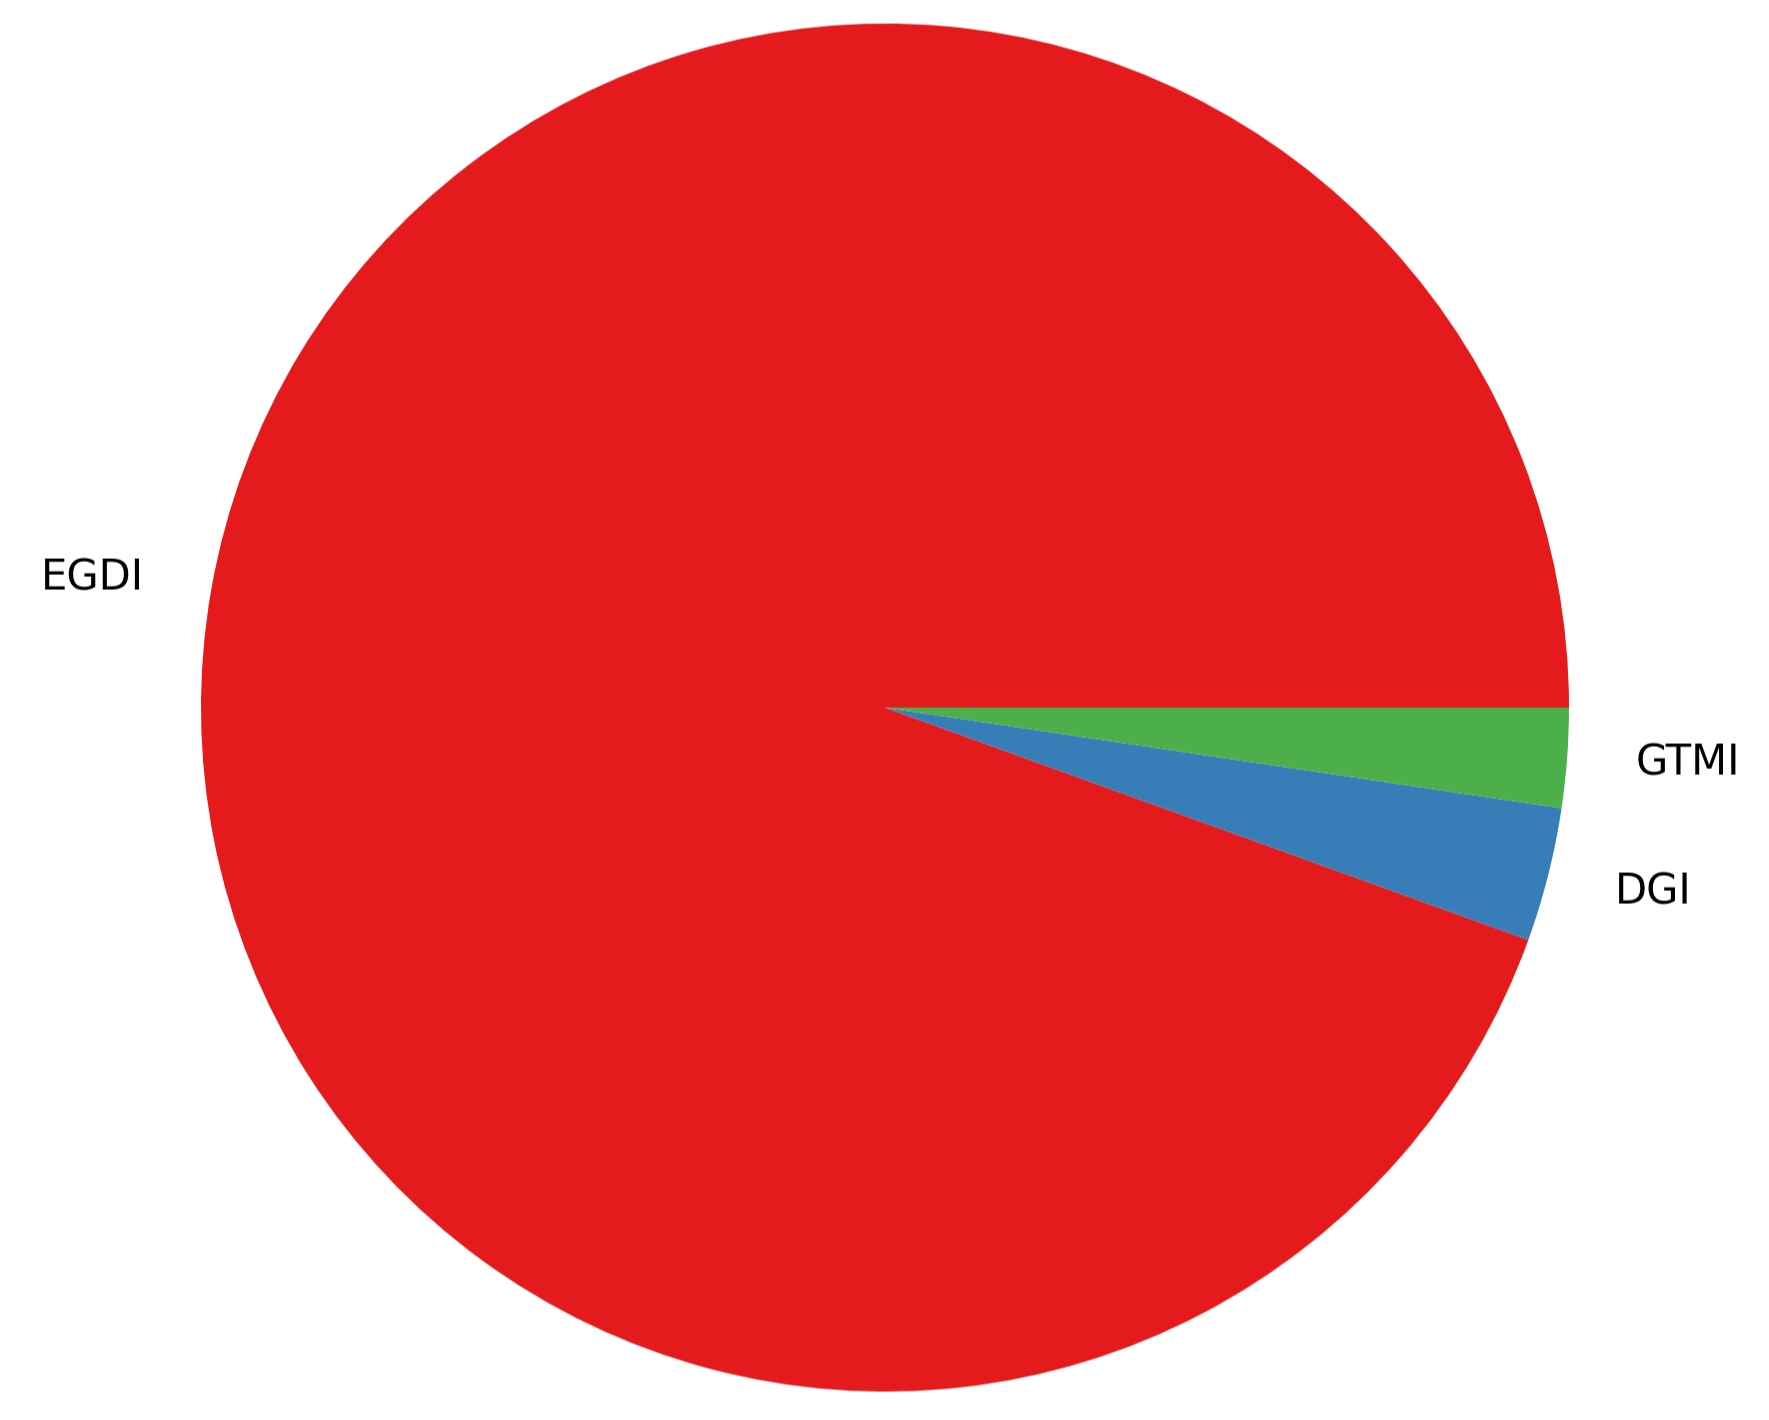
\includegraphics[width=0.6\linewidth]{figuras/indices/indices_google_academico}
	\label{fig:indices_google_academico}
	\\ \footnotesize{Fonte: elaboração própia.}
\end{figure}

Dentre os índices com abrangência global – EGDI, GTMI e DGI – optou-se pelo primeiro. Embora o GTMI do Banco Mundial e o DGI da OECD também ofereçam visões valiosas sobre a maturidade do governo digital, o EGDI da ONU foi o escolhido devido a maior quantidade de material .

O EGDI apresenta o estado de desenvolvimento de governo eletrônico dos Estados membros da ONU. O índice incorpora as características de acesso, tais como níveis de infraestrutura e educacional para mostrar como um país está usando as tecnologias de informação para promover acesso e inclusão do seu povo \cite{ONU_EGDI}.

\cite{ONU_EGDI} afirma que o EGDI é uma mensuração composta formada por 3 importantes dimensões do governo eletrônico: provisão de serviços online, conectividade de telecomunicação e capacidade humana.

Os componentes do EGDI são:

\begin{figure}[H]
	\centering
	\caption{Os três componentes do EGDI}
	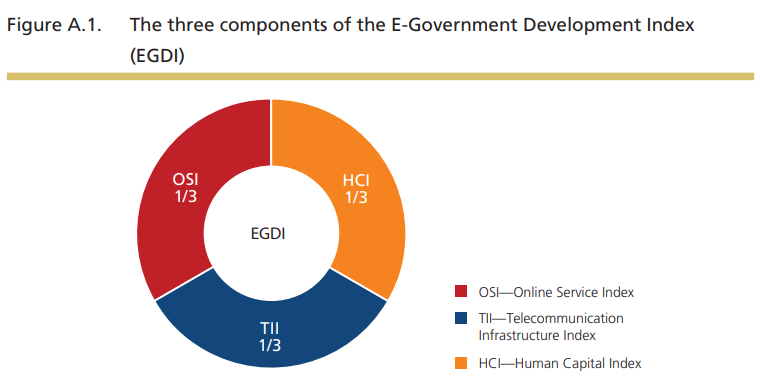
\includegraphics[width=1\linewidth]{figuras/egdi/egdi_componentes.png}
	\label{fig:egdi_componentes}
	\footnotesize{Fonte: \cite{ONU_EGDI_methodology}}
\end{figure}

A figura \ref{fig:boxplot_egov_global} contém um diagrama de caixa que representa o EGDI global.

\begin{figure}[H]
	\centering
	\caption{E-Government Development Index global em 2024}
	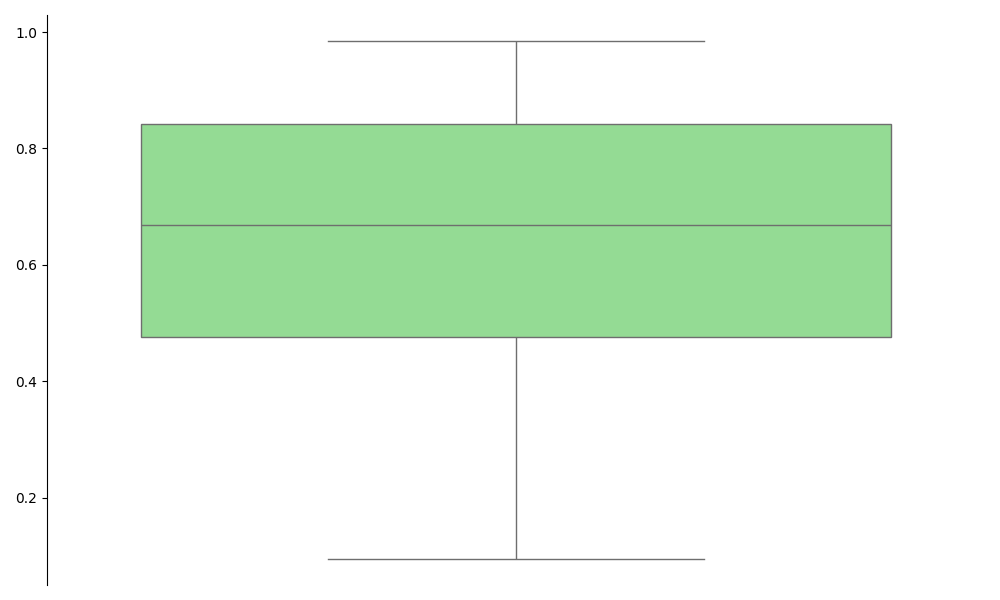
\includegraphics[width=1\linewidth]{figuras/egdi/boxplot_egov_global.png}
	\label{fig:boxplot_egov_global}
	\footnotesize{Fonte: baseado em \cite{ONU_EGDI_mapa}.}
\end{figure}

A linha central na caixa indica que a mediana do índice é de aproximadamente 0.65. A caixa em si, que representa os 50\% centrais dos dados, se estende de cerca de 0.48 a 0.83, mostrando a variação dos índices na maioria dos países. As linhas verticais, conhecidas como "bigodes", demonstram a amplitude total dos dados, que vai de aproximadamente 0.1 a quase 1.0. A distribuição do índice parece ser relativamente simétrica, sem um viés perceptível para valores mais altos ou mais baixos, e o gráfico não identifica a presença de valores discrepantes (outliers) extremos.

\section{E-Participation Index}
\label{epart}

\cite{ONU_EGDI} argumenta que o \textbf{E-Participation Index} deriva do EGDI como índice suplementar ao relatório \textbf{E-Government Survey}. Os componentes do índice são: \textbf{E-information}, \textbf{E-consultation} e \textbf{E-decision-making}. 

\textbf{E-information} fala sobre a facilitação da participação dos cidadãos via informações públicas e acesso a informação sem necessidade de pedido ou sob demanda. \textbf{E-consultation} diz respeito ao engajamento dos cidadãos em contribuições e deliberações sobre políticas publicas e serviços públicos. \textbf{E-decision-making} engloba o empoderamento dos cidadãos via a opção de coparticipação na elaboração de políticas e coprodução de componentes de serviços e entrega de modalidades.

\cite{ONU_EGDI} esclarece que o \textbf{E-Participation Index} de um país reflete os mecanismos do índice que são empregados pelo governo quando se faz comparações com todos outros países. 

O propósito dessa medição não é prescrever qualquer prática especificam, no entanto oferece perspectivas de como países diferentes estão usando ferramentas online para promover interação entre o governo e seu povo, bem como, entre as pessoas para benefícios de todos.

A figura \ref{fig:boxplot_epart_global} contém um diagrama de caixa que representa o \textbf{E-Participation Index} global.

\begin{figure}[H]
	\centering
	\caption{E-Participation Index global em 2024}
	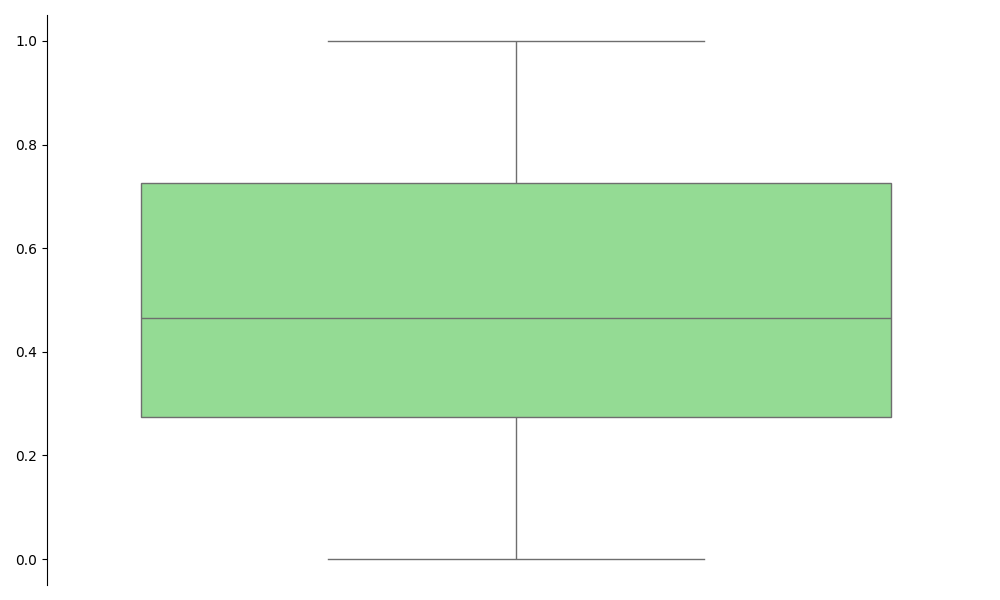
\includegraphics[width=1\linewidth]{figuras/egdi/boxplot_epart_global.png}
	\label{fig:boxplot_epart_global}
	\footnotesize{Fonte: baseado em \cite{ONU_EGDI_mapa}.}
\end{figure}

A figura \ref{fig:boxplot_epart_global} revela que a mediana do índice é de aproximadamente 0.47, indicando que metade dos países avaliados se encontra acima desse valor. A caixa do gráfico abrange o intervalo entre 0.28 e 0.72, onde estão concentrados 50\% dos países. A amplitude total dos índices é considerável, variando de 0.0 a 1.0. A distribuição se apresenta como relativamente simétrica, sem uma concentração significativa de países nas extremidades dos dados, e não há indícios de valores discrepantes (outliers).

\section{Online Service Index}
\label{osi}

A figura \ref{fig:boxplot_osi_global} contém um diagrama de caixa que representa o \textbf{E-Participation Index} global.

\begin{figure}[H]
	\centering
	\caption{Online Service Index global em 2024}
	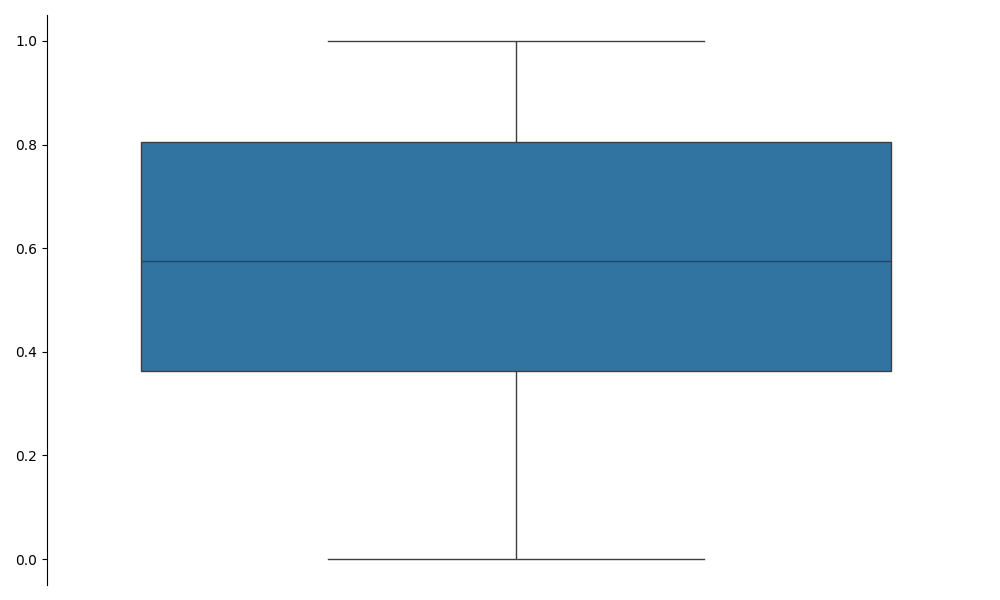
\includegraphics[width=1\linewidth]{figuras/egdi/boxplot_osi_global.png}
	\label{fig:boxplot_osi_global}
	\footnotesize{Fonte: baseado em \cite{ONU_EGDI_mapa}.}
\end{figure}

A figura \ref{fig:boxplot_osi_global} revela que a mediana do índice de serviços online é de aproximadamente 0.58. A caixa principal do gráfico indica que 50\% dos países têm índices que variam entre 0.38 e 0.81. A amplitude total dos dados é vasta, indo de 0.0 a 1.0, o que demonstra uma grande disparidade nos níveis de serviços online oferecidos globalmente. A distribuição dos dados é relativamente simétrica e, assim como nos gráficos anteriores, não há outliers visíveis.

\section{Human Capital Index em 2024}
\label{hci}

\cite{ONU_EGDI_methodology} afirma que \textbf{Human Capital Index} tem 4 indicadores: taxa bruta de matrícula, letramento adulto, anos de escolarização esperados e média de anos de escolaridade. 

A taxa bruta de matrícula é medida como a combinação entre a taxa de matrícula nas educações primárias, secundários e terciárias. Letramento adulto é medido como o percentual de pessoas com pelos menos 15 anos de idade que entendem e sabem ler e escrever um frase curta simples na sua vida padrão.

Os anos de escolarização esperados é o número total de anos de escolarização que crianças de certa idade podem esperar ter no futuro, presumindo que a probabilidade de a criança de qualquer idade estiver na escola correspondendo à idade da taxa de matrícula atual.

A média de anos de escolaridade fornece o número médio de anos de educação concluídos pela população adulta de um país (25 anos ou mais), excluindo os anos gastos repetindo séries. 

A figura \ref{fig:boxplot_hci_global} contém um diagrama de caixa que representa o \textbf{E-Participation Index} global.

\begin{figure}[H]
	\centering
	\caption{Human Capital Index global em 2024}
	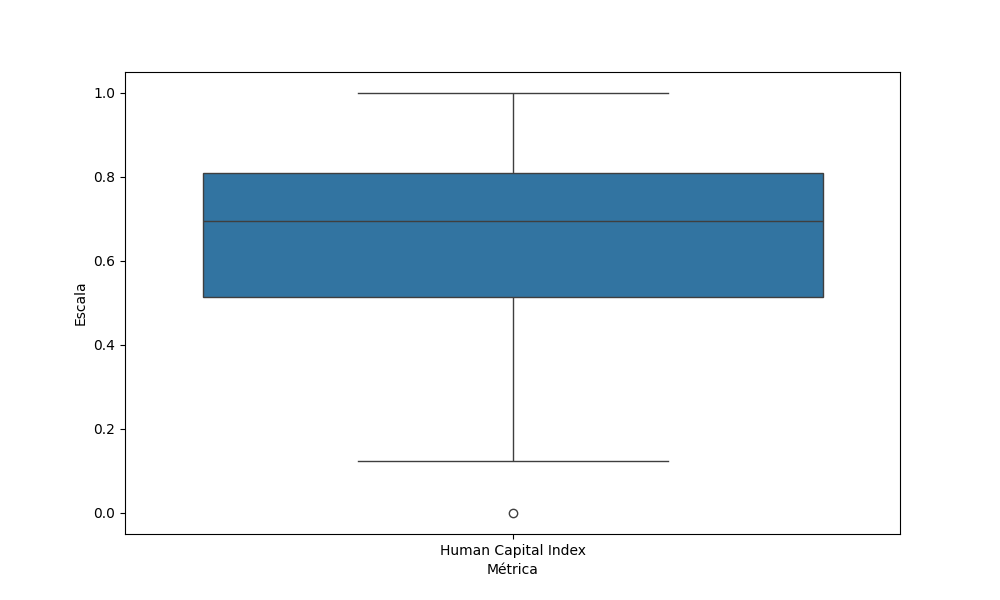
\includegraphics[width=1\linewidth]{figuras/egdi/boxplot_hci_global.png}
	\label{fig:boxplot_hci_global}
	\footnotesize{Fonte: baseado em \cite{ONU_EGDI_mapa}.}
\end{figure}

A figura \ref{fig:boxplot_hci_global} mostra que a mediana do índice de capital humano é de aproximadamente 0.70. A caixa principal, que concentra os 50\% centrais dos dados, indica que a maioria dos países tem um índice que varia entre 0.52 e 0.81. A amplitude dos dados é ampla, indo de cerca de 0.13 a 1.0. A distribuição se apresenta como relativamente simétrica, e, diferentemente dos gráficos anteriores, este diagrama aponta a existência de um outlier, um valor discrepante isolado, localizado próximo ao zero no eixo vertical, indicando um país com um índice de capital humano excepcionalmente baixo em comparação com os demais.

\section{Telecommunication Infrastructure Index em 2024}
\label{tii}

\cite{ONU_EGDI_methodology} afirma que o \textbf{Telecommunication Infrastructure Index} tem 5 componentes: usuário de internet, assinatura de banda larga fixa, assinatura de banda larga sem fio, assinatura de telefone fixo e assinatura de dados móveis.

A figura \ref{fig:boxplot_tci_global} contém um diagrama de caixa que representa o \textbf{E-Participation Index} global.

\begin{figure}[H]
	\centering
	\caption{Telecommunication Infrastructure Index global em 2024}
	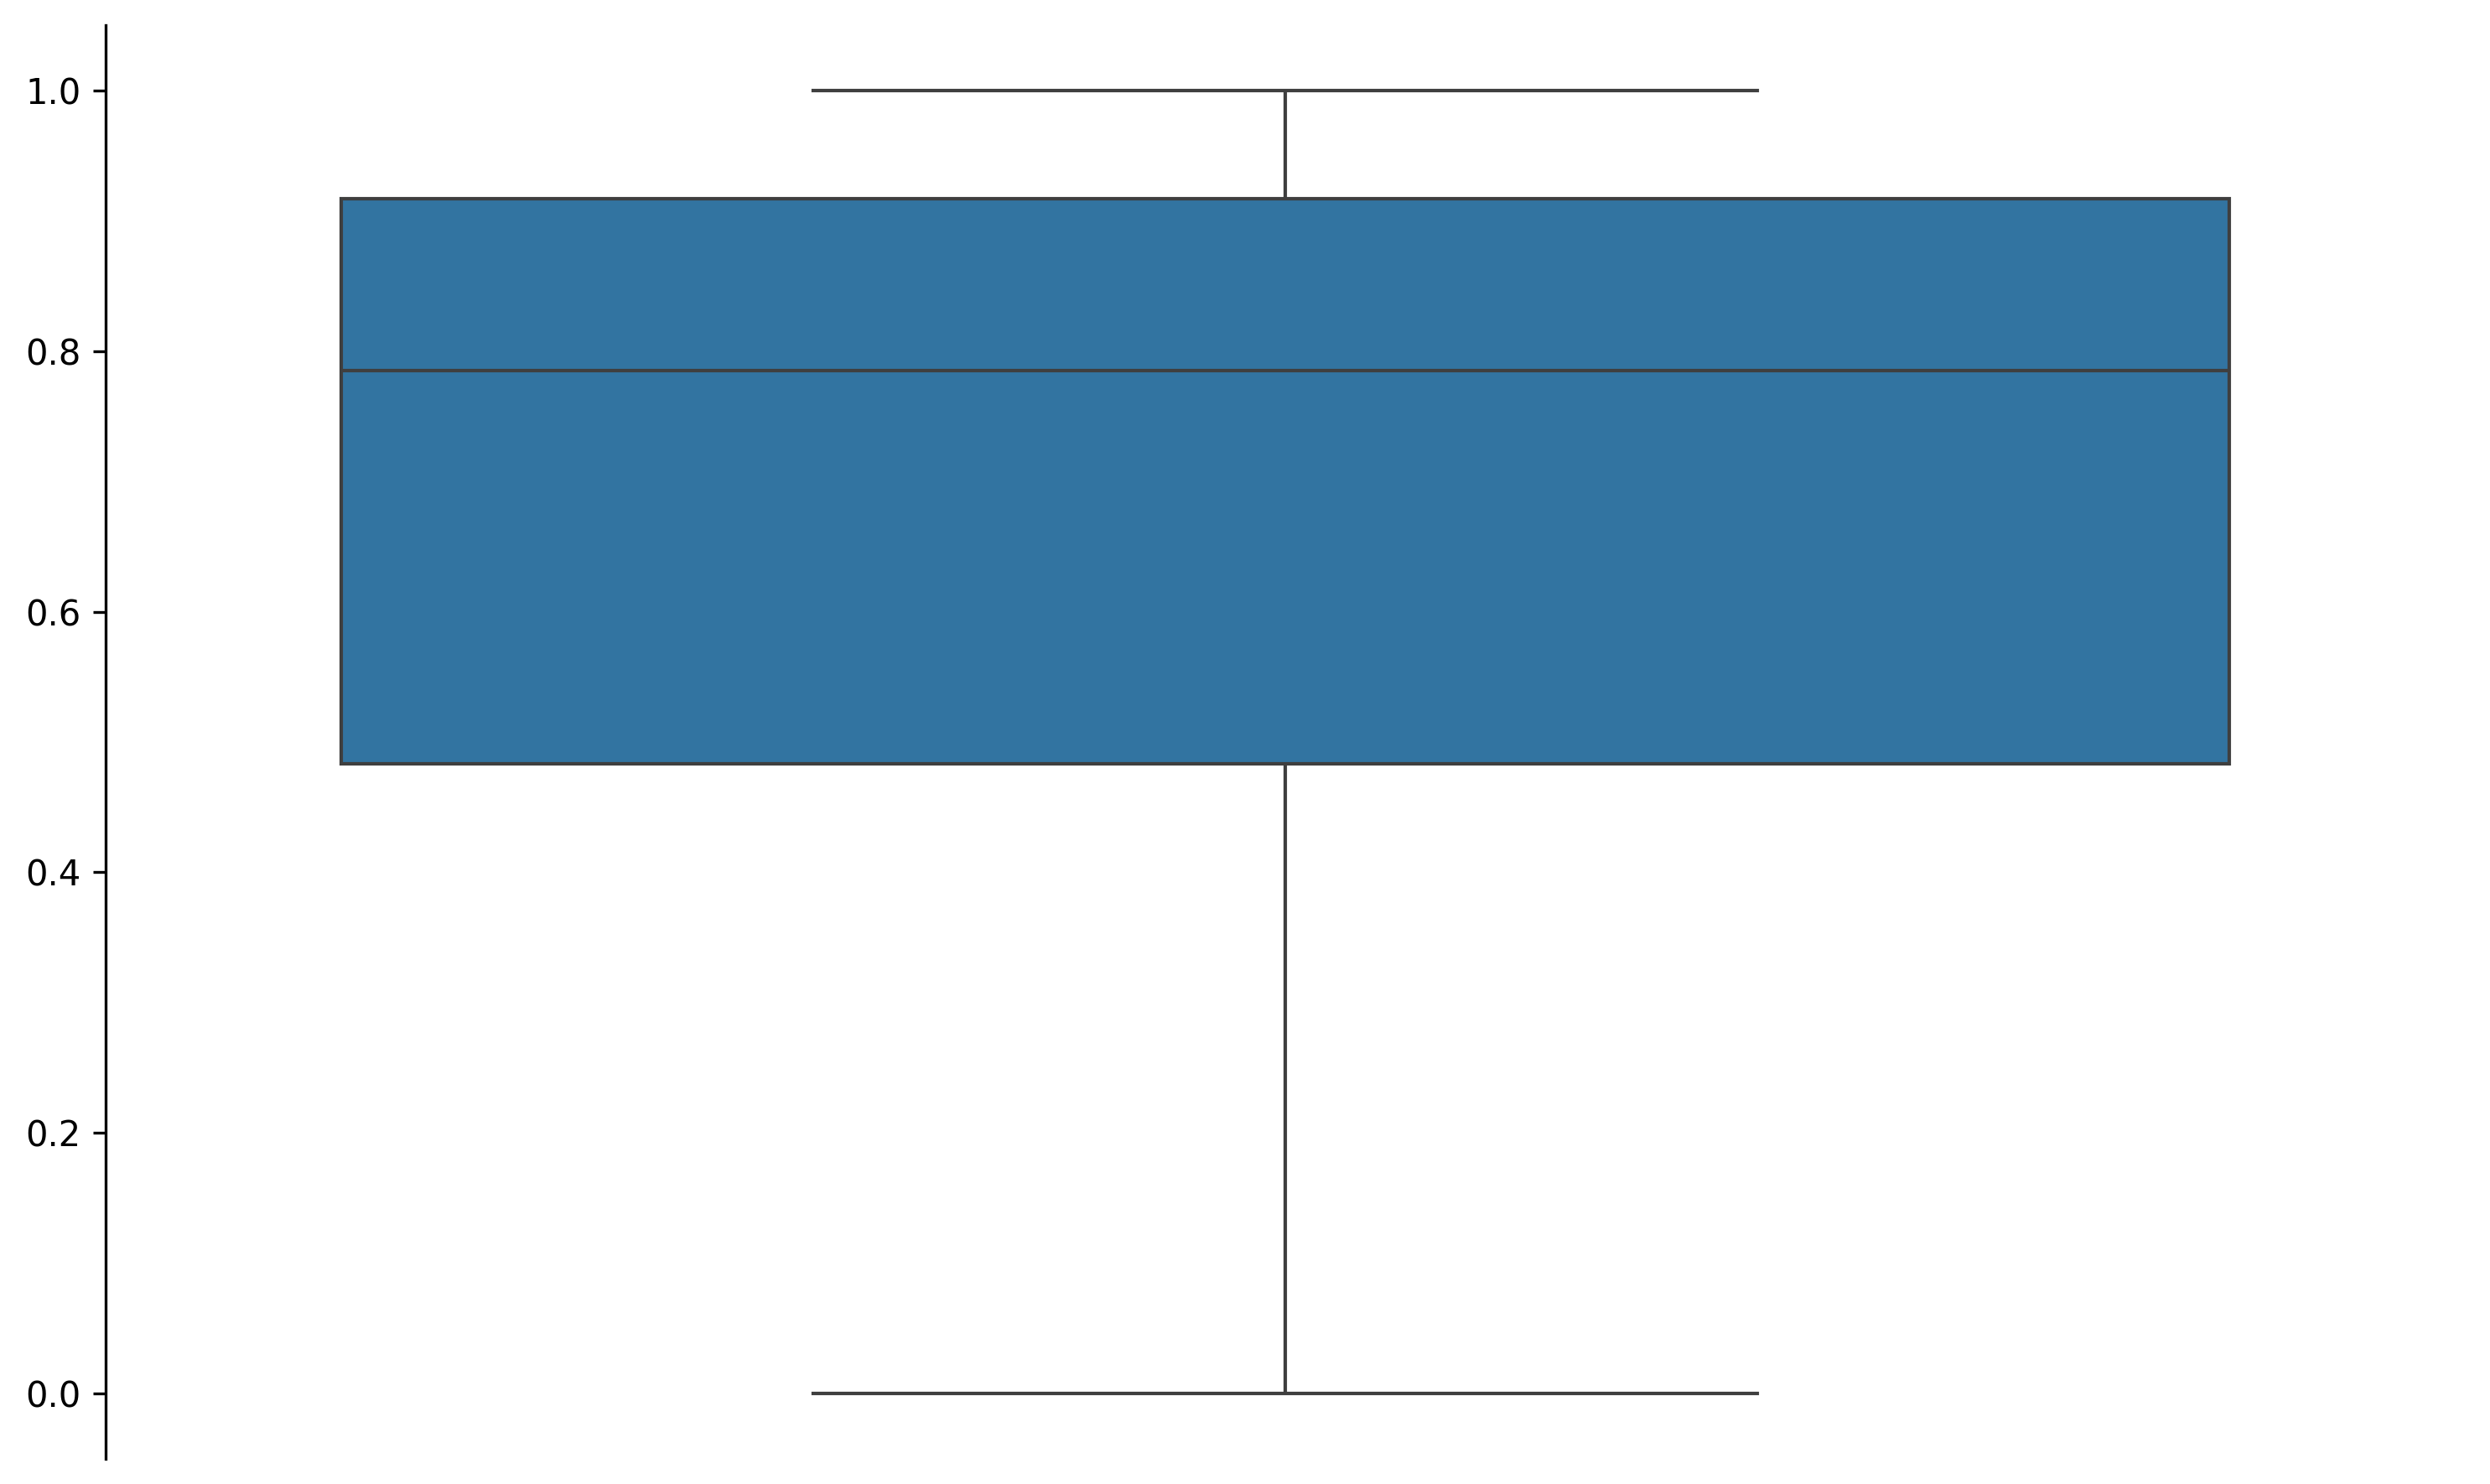
\includegraphics[width=1\linewidth]{figuras/egdi/boxplot_tci_global.png}
	\label{fig:boxplot_tci_global}
	\footnotesize{Fonte: baseado em \cite{ONU_EGDI_mapa}.}
\end{figure}

A figura \ref{fig:boxplot_tci_global} mostra que a mediana do índice de infraestrutura de telecomunicações está em cerca de 0.80, indicando que metade dos países possui um índice superior a esse valor. A caixa do gráfico, que representa os 50\% centrais dos dados, abrange o intervalo entre aproximadamente 0.50 e 0.90. A amplitude total dos dados varia de 0.0 a 1.0. A distribuição dos dados é relativamente simétrica e, assim como na maioria dos gráficos anteriores, não há outliers visíveis.

\section{Coeficiente de correlação: EGDI e E-Participation comparadas com outras variáveis}

Ao analisar os dados do \href{https://publicadministration.un.org/egovkb/en-us/About/Overview/-E-Government-Development-Index}{EGDI}, foi notado que tanto democracias consolidadas, quanto autocracias tem um EGDI alto. O critério para entender quais países são democráticos ou autocráticos foi a figura \ref{fig:electoral-democracy-index}. 

\begin{figure}[H]
	\centering
	\caption{Índice da democracia eleitoral}
	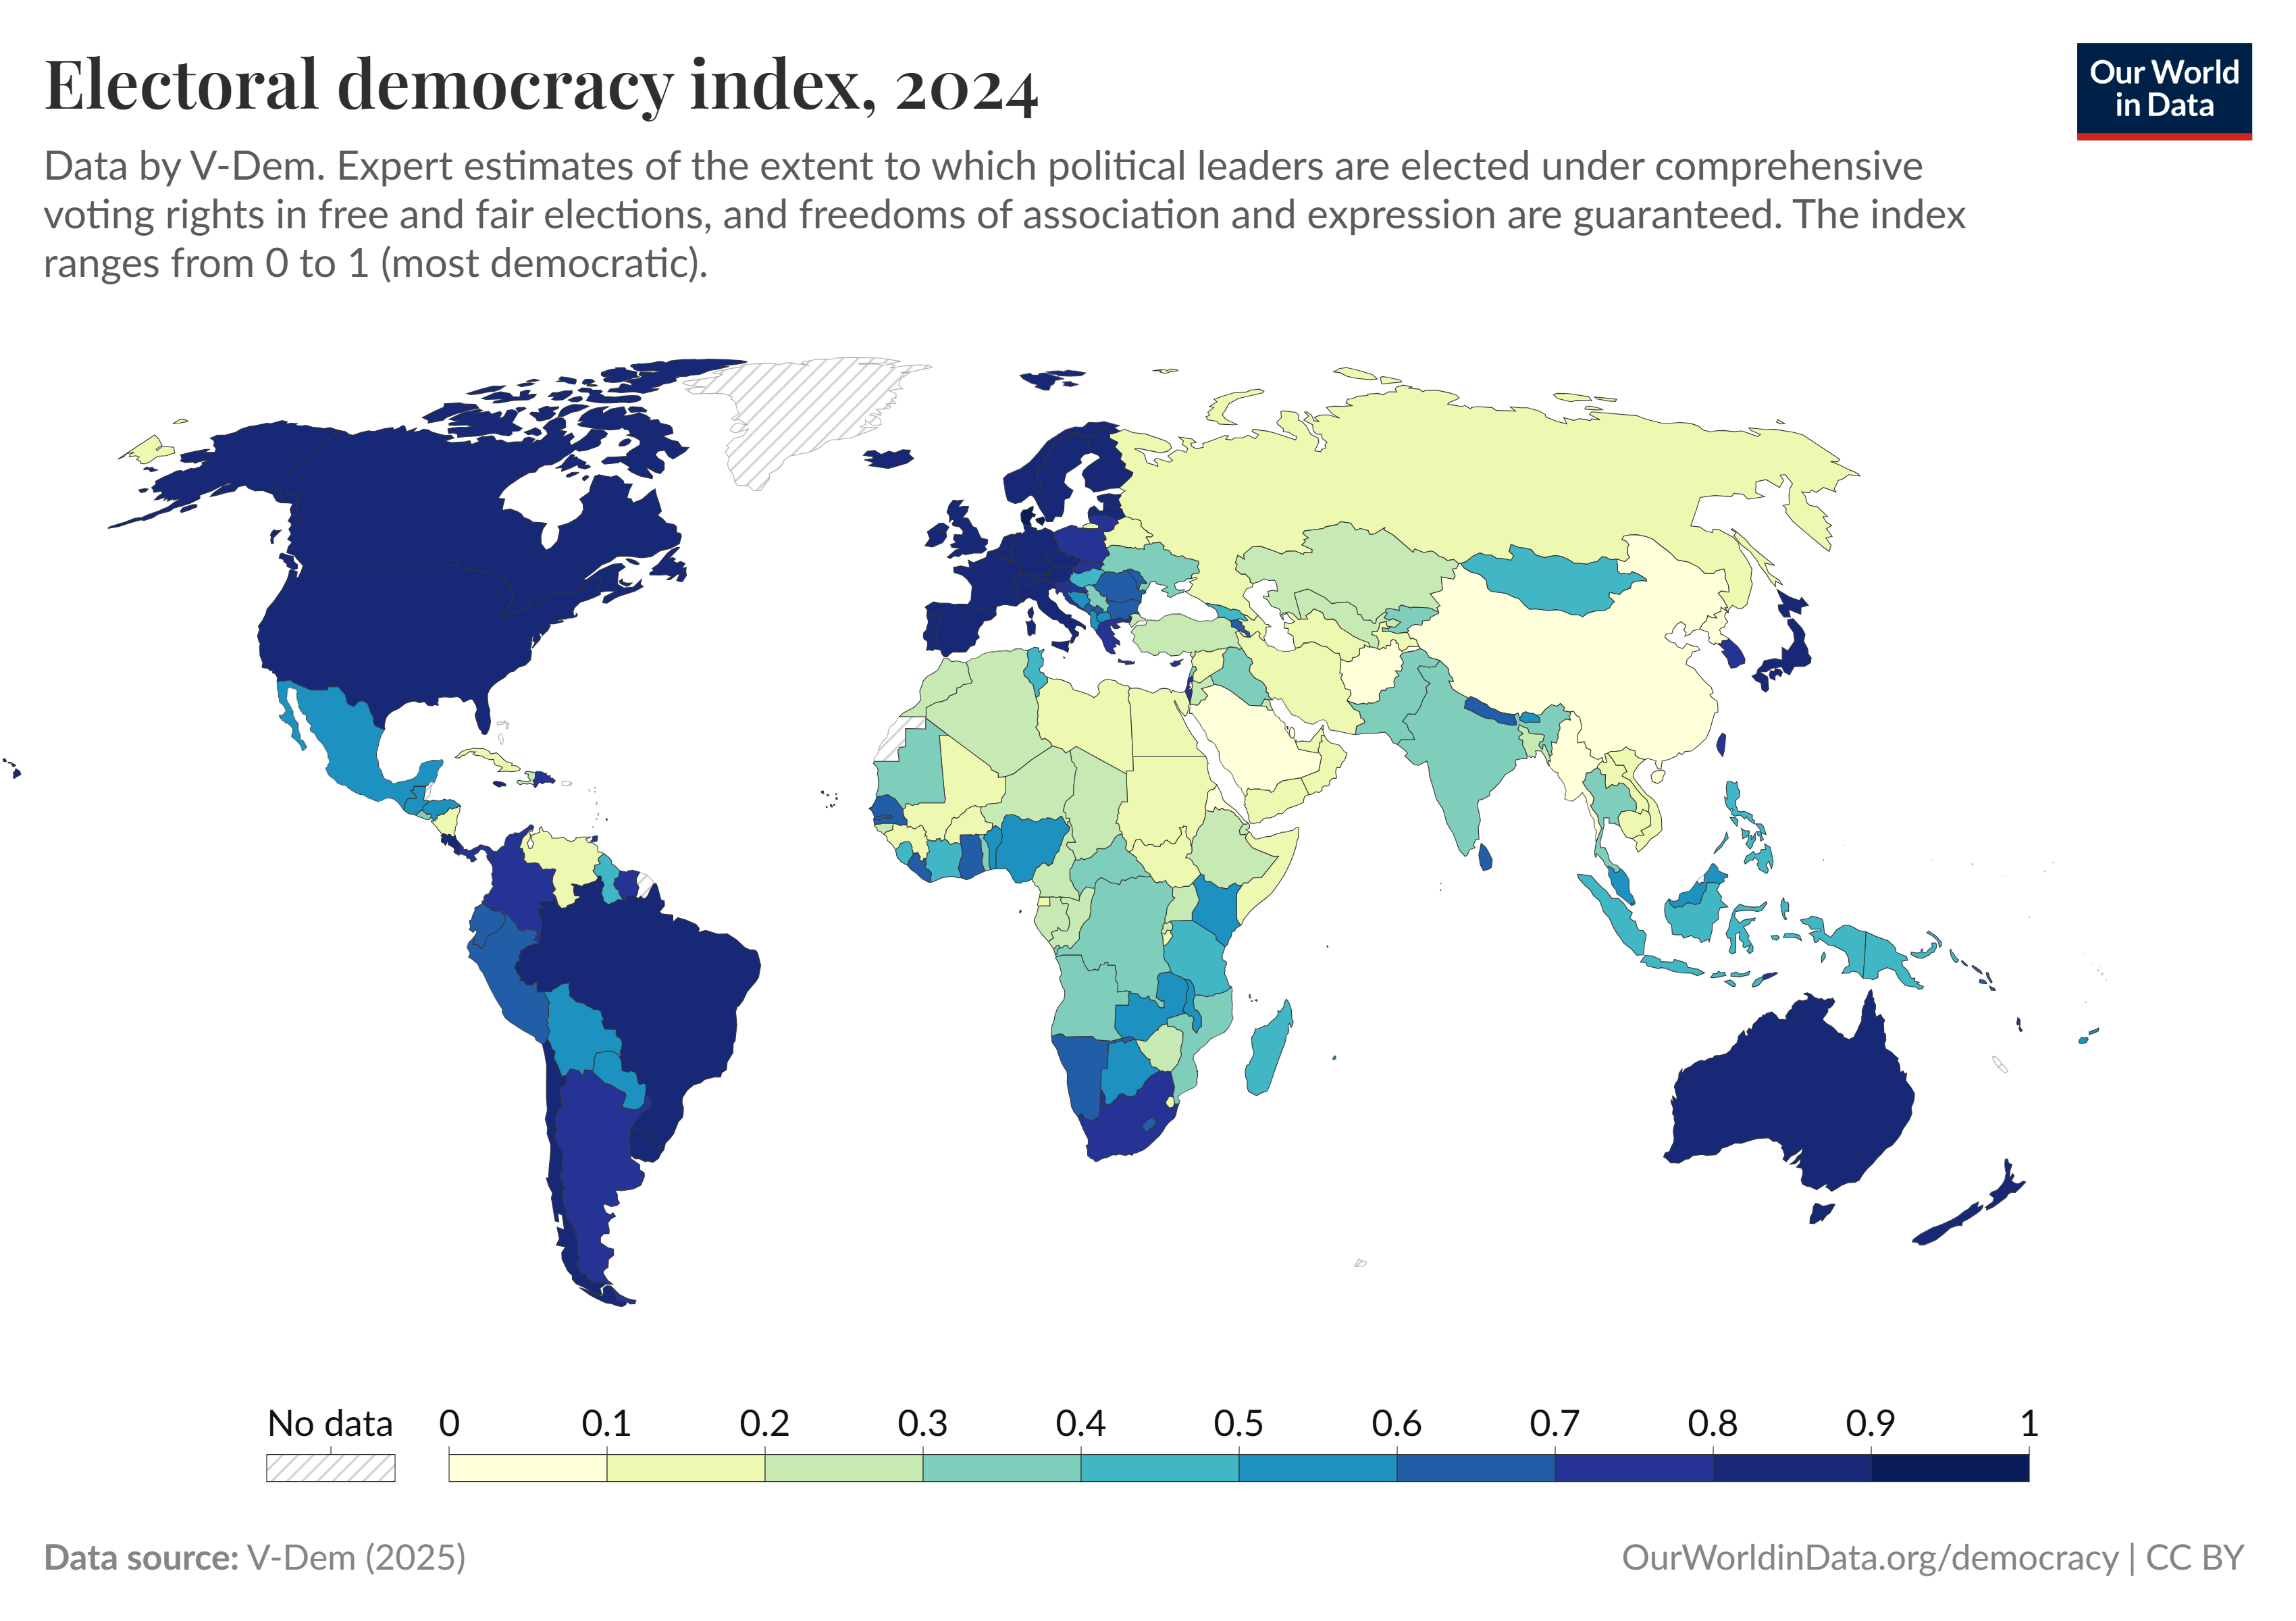
\includegraphics[width=1\linewidth]{figuras/democracia/electoral-democracy-index.png}
	\label{fig:electoral-democracy-index}
	\footnotesize{Fonte: \cite{electoral_democracy_index}}
\end{figure}

Nota-se que o Brasil é considerado uma democracia eleitoral, estando na minoria numérica de países democráticas (88), conforme exposto por \cite{nord2025democracy}, contra 91 autocracias no ano de 2025, haja vista o relatótio \href{https://www.v-dem.net/documents/60/V-dem-dr__2025_lowres.pdf}{DEMOCRACY REPORT 2025: 25 Years of Autocratization – Democracy Trumped?}

Outro fator chamou atenção: há EGDI alto em países tanto autocráticos, quanto democráticos que têm PIB \textit{per capita} alto, conforme comparação inicial dos \href{https://data.worldbank.org/indicator/NY.GDP.PCAP.PP.KD}{com o PIB \textit{per capita} dos países}. 

Adicionalmente, ao avaliar o gasto públicos dos governos apresentado pela OECD e resumido na figura \ref{fig:government-spending-by-function}, um detalhe foi chamativo.

\begin{figure}[H]
	\centering
	\caption{Gastos gerais governamentais (\% do PIB)}
	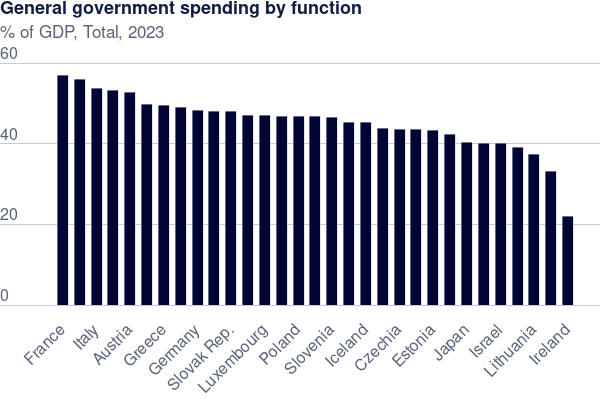
\includegraphics[width=1\linewidth]{figuras/government_spending/government-spending-by-function}
	\label{fig:government-spending-by-function}
	\footnotesize{Fonte: \cite{global_gov_spending_function}}
\end{figure}

Notou-se que os páises democráticos (membros da OECD) que têm EGDI altos tem, coincidentemente, altos gastos públicos e que eles representam parte considerável do PIB. A França e a Itália lideram com uma pequena diferença da 2ª para a 1ª. Outro fato é notório é maioria dos países gastam mais de 40\% do PIB.

Com base nos parágrafos anteriores, um questionamento surgiu: qual é relação entre EGDI e \textbf{E-Participation Index} com o índice de democracia eleitoral do \href{https://www.v-dem.net/}{V-Dem}, com o PIB \textit{per capita} e com os gastos públicos (\% do PIB.) Para descobrir qual tipo de coeficiente de correlação usar, fez-se diagramas de dispersão. Caso haja linearidade, usar-se-á Pearson; caso contrário Spearman.

\subsection{Análise geral com o EGDI e E-Participation Index}

Analisar-se-á o aspecto geral usando o EGDI e o \textbf{E-Participation Index}, estudando como essas variáveis se comportam em diagramas de dispersão e coeficientes de correlação quando comparada com outras variáveis.

\subsubsection{EGDI e PIB \textit{per capita} PPC}

\begin{figure}[H]
	\centering
	\caption{Diagrama de Dispensao: EGDI e PIB \textit{per capita} PPC}
	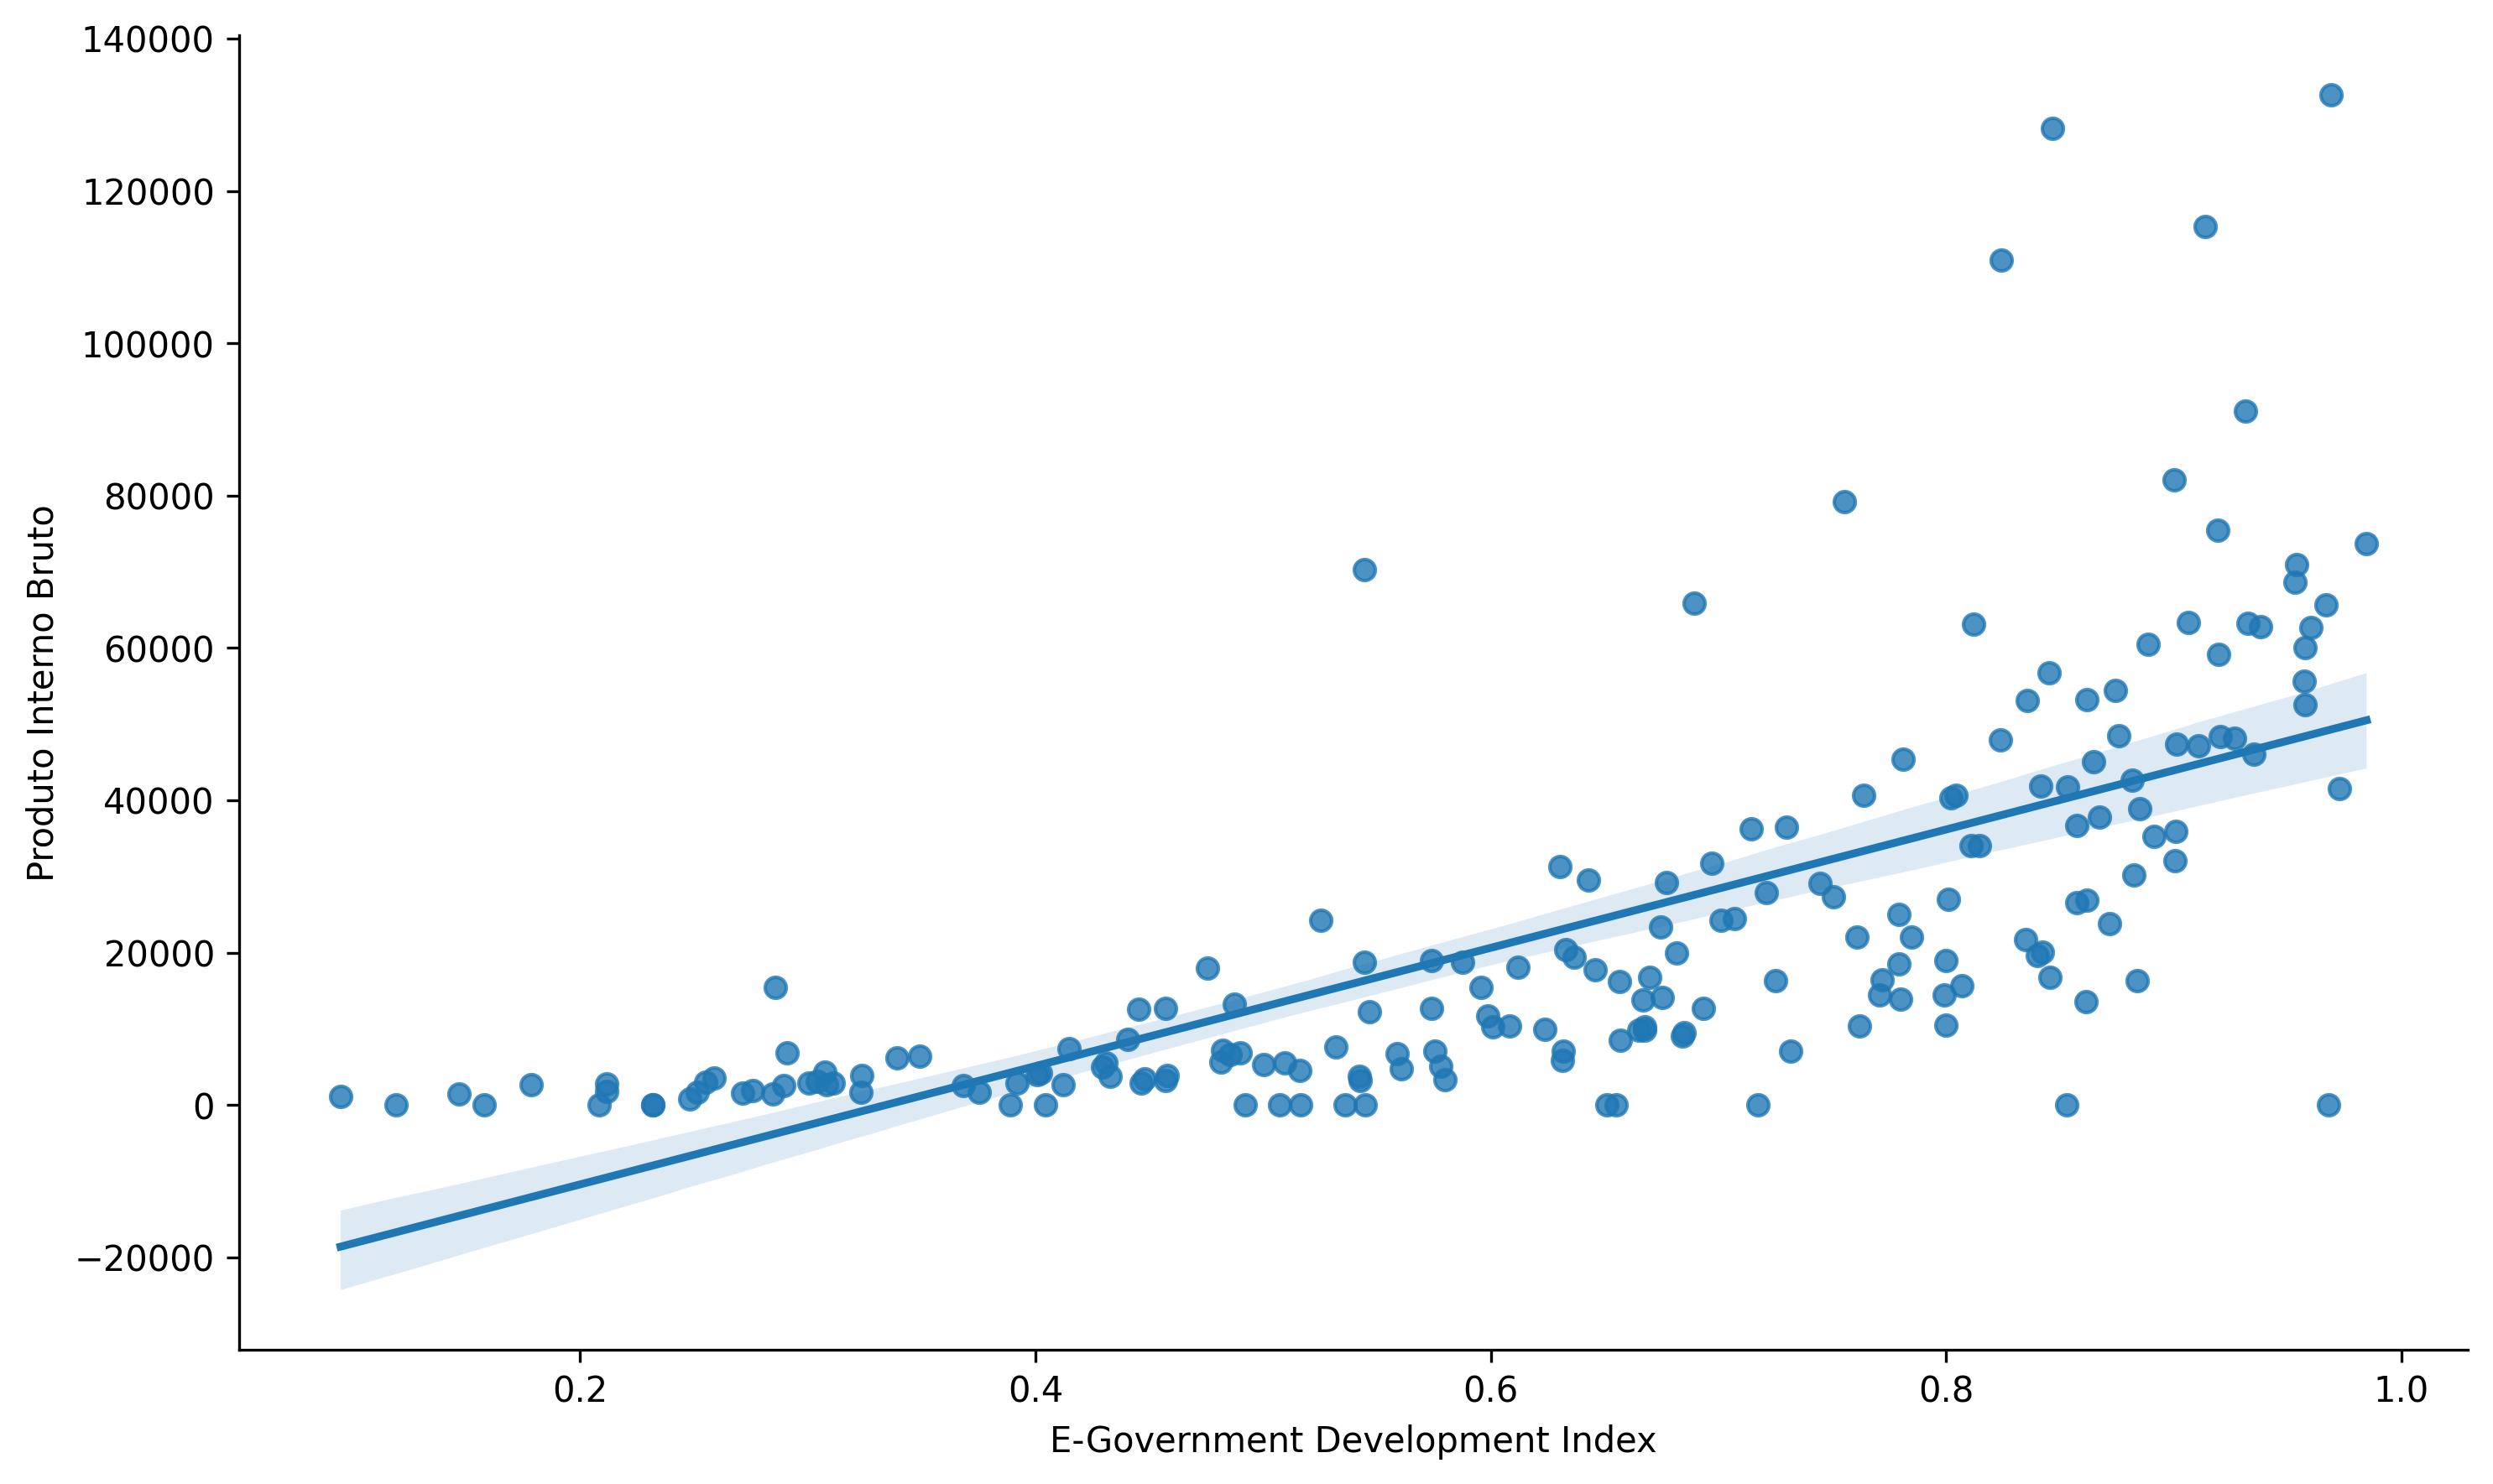
\includegraphics[width=1\linewidth]{figuras/egdi/dispensao_egov_pib}
	\label{fig:dispensao_egov_pib}
	\footnotesize{Fonte: \cite{ONU_EGDI} e \cite{WB_pib_per_capita_países}}
\end{figure}

Para compreender melhor o diagrama de dispersão, foi usado o coeficiente de correlação de Spearman. A sua escolha foi motivada pela grande presença de pontos extremos. O coeficiente de correlação encontrada foi 0.82. Devido ao coeficiente, os PIB \textit{per capita} PPC e o \textbf{E-Government Index} tendem a crescer juntos.

\subsubsection{E-Participation Index e PIB \textit{per capita} PPC}

\begin{figure}[H]
	\centering
	\caption{Diagrama de Dispensao: E-Participation Index e PIB \textit{per capita} PPC}
	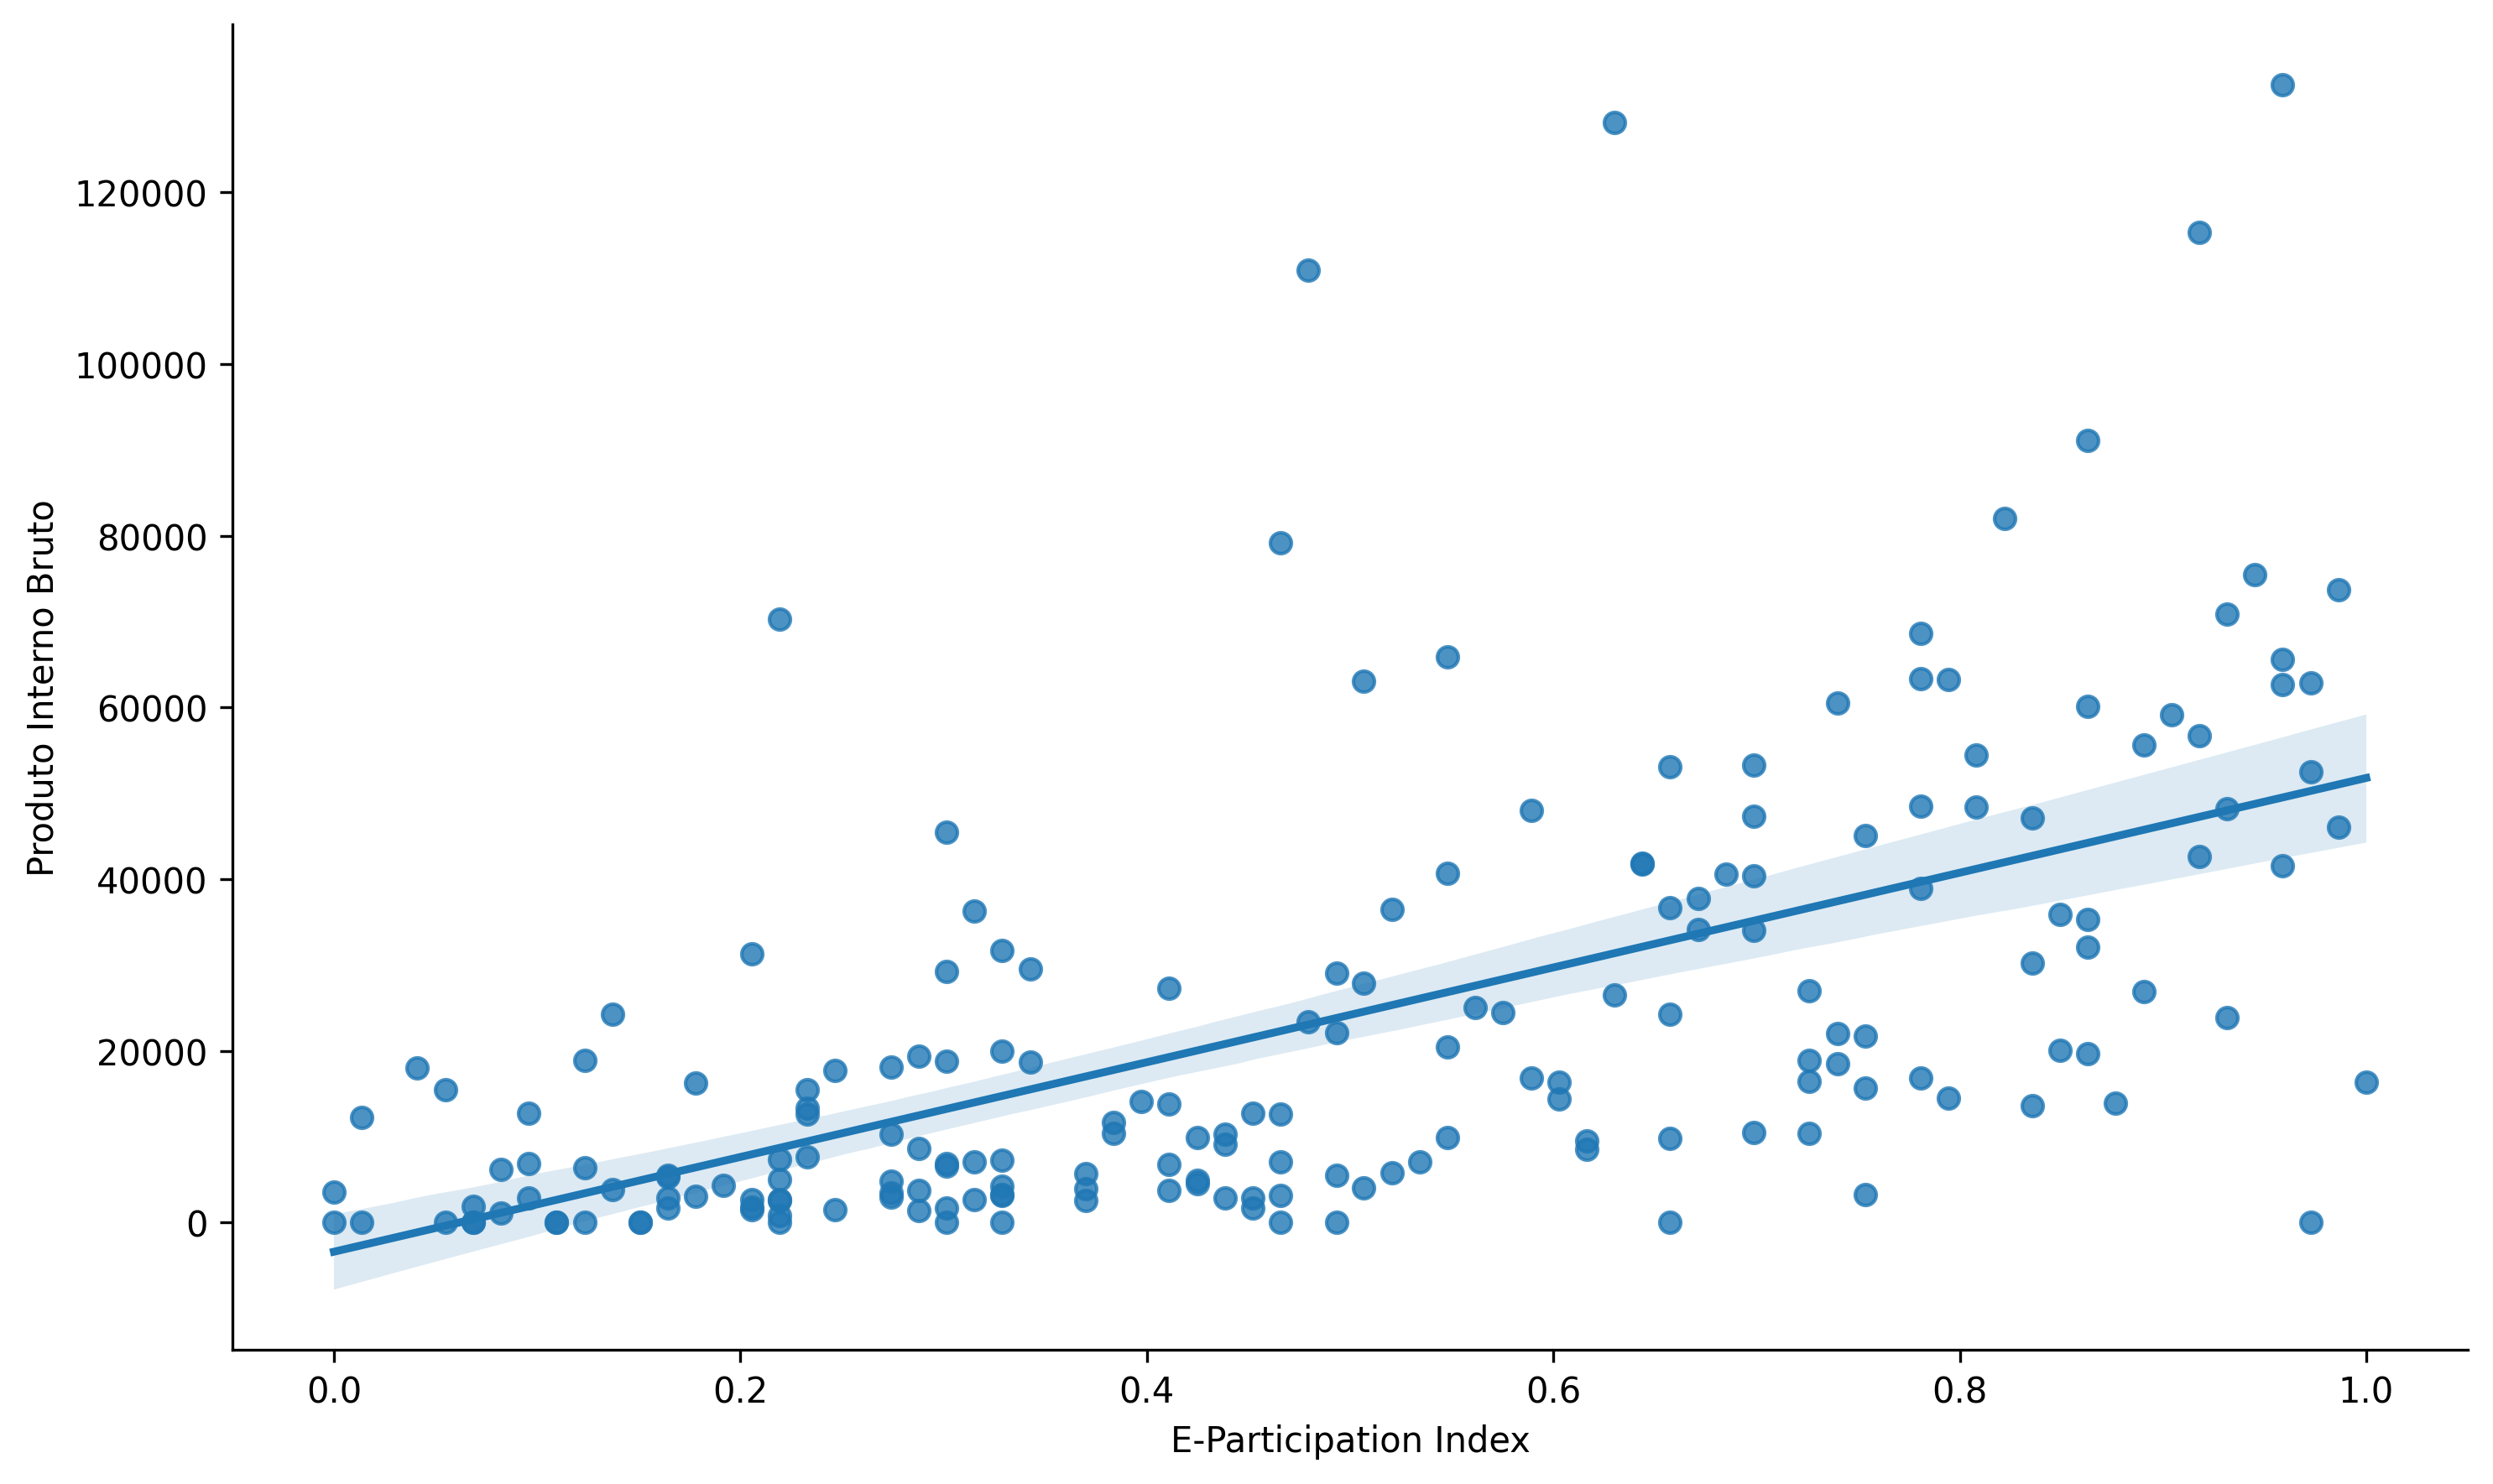
\includegraphics[width=1\linewidth]{figuras/egdi/dispensao_epart_pib}
	\label{fig:dispensao_epart_pib}
	\footnotesize{Fonte: \cite{ONU_EGDI_mapa} e \cite{WB_pib_per_capita_países}}
\end{figure}

Para compreender melhor o diagrama de dispersão, foi usado o coeficiente de correlação de Spearman. A sua escolha foi motivada pela grande presença de pontos extremos. O coeficiente de correlação encontrada foi 0.67. Devido ao coeficiente, os PIB \textit{per capita} PPC e o \textbf{E-Participation Index} tendem a crescer juntos.

\subsubsection{EGDI e índice de democracia eleitoral}

\begin{figure}[H]
	\centering
	\caption{Diagrama de Dispensao: EGDI e índice de democracia eleitoral}
	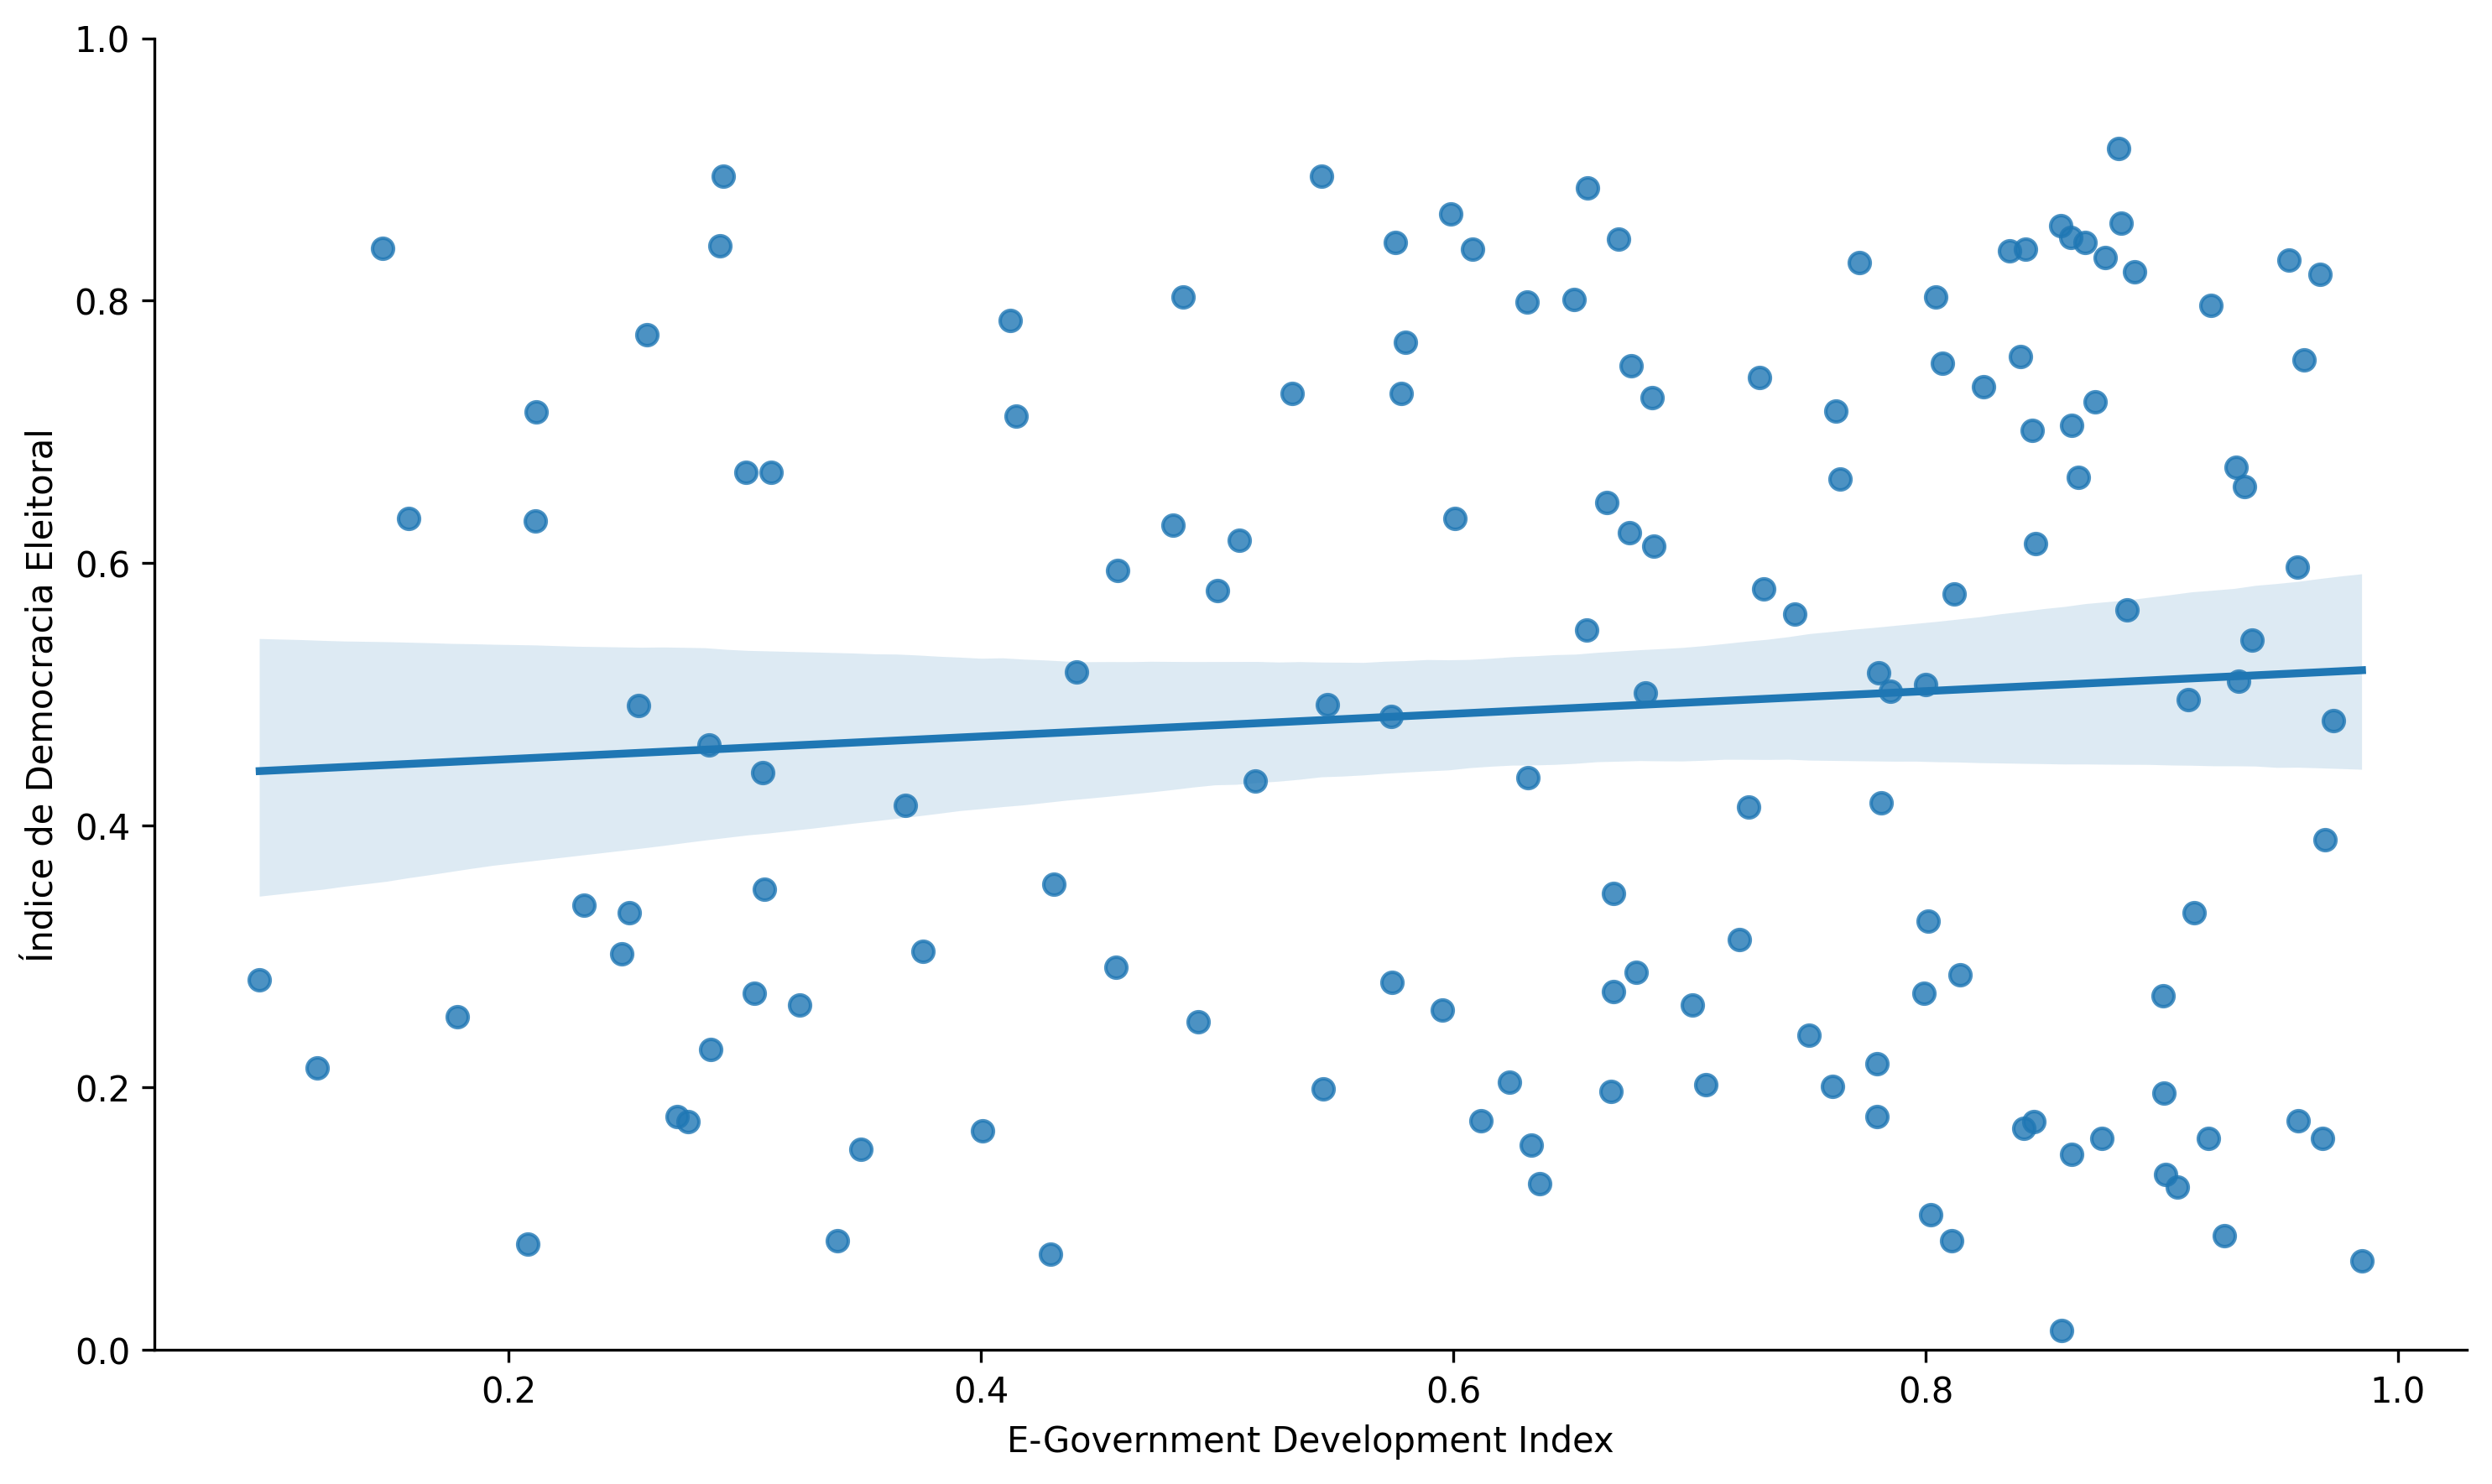
\includegraphics[width=1\linewidth]{figuras/egdi/dispersao_egov_indicedemocracia}
	\label{fig:dispersao_egov_indicedemocracia}
	\footnotesize{Fonte: \cite{ONU_EGDI} e \cite{electoral_democracy_index}}
\end{figure}

Para compreender melhor o diagrama de dispersão, foi usado o coeficiente de correlação de Spearman. A sua escolha foi motivada pela grande presença de pontos extremos. O coeficiente de correlação encontrada foi 0.04. Os índice de democracia eleitoral e o \textbf{E-Government Index} são variáveis independentes.

\subsubsection{E-Participation Index e índice de democracia eleitoral}

\begin{figure}[H]
	\centering
	\caption{Diagrama de Dispensao: E-Participation Index e índice de democracia eleitoral}
	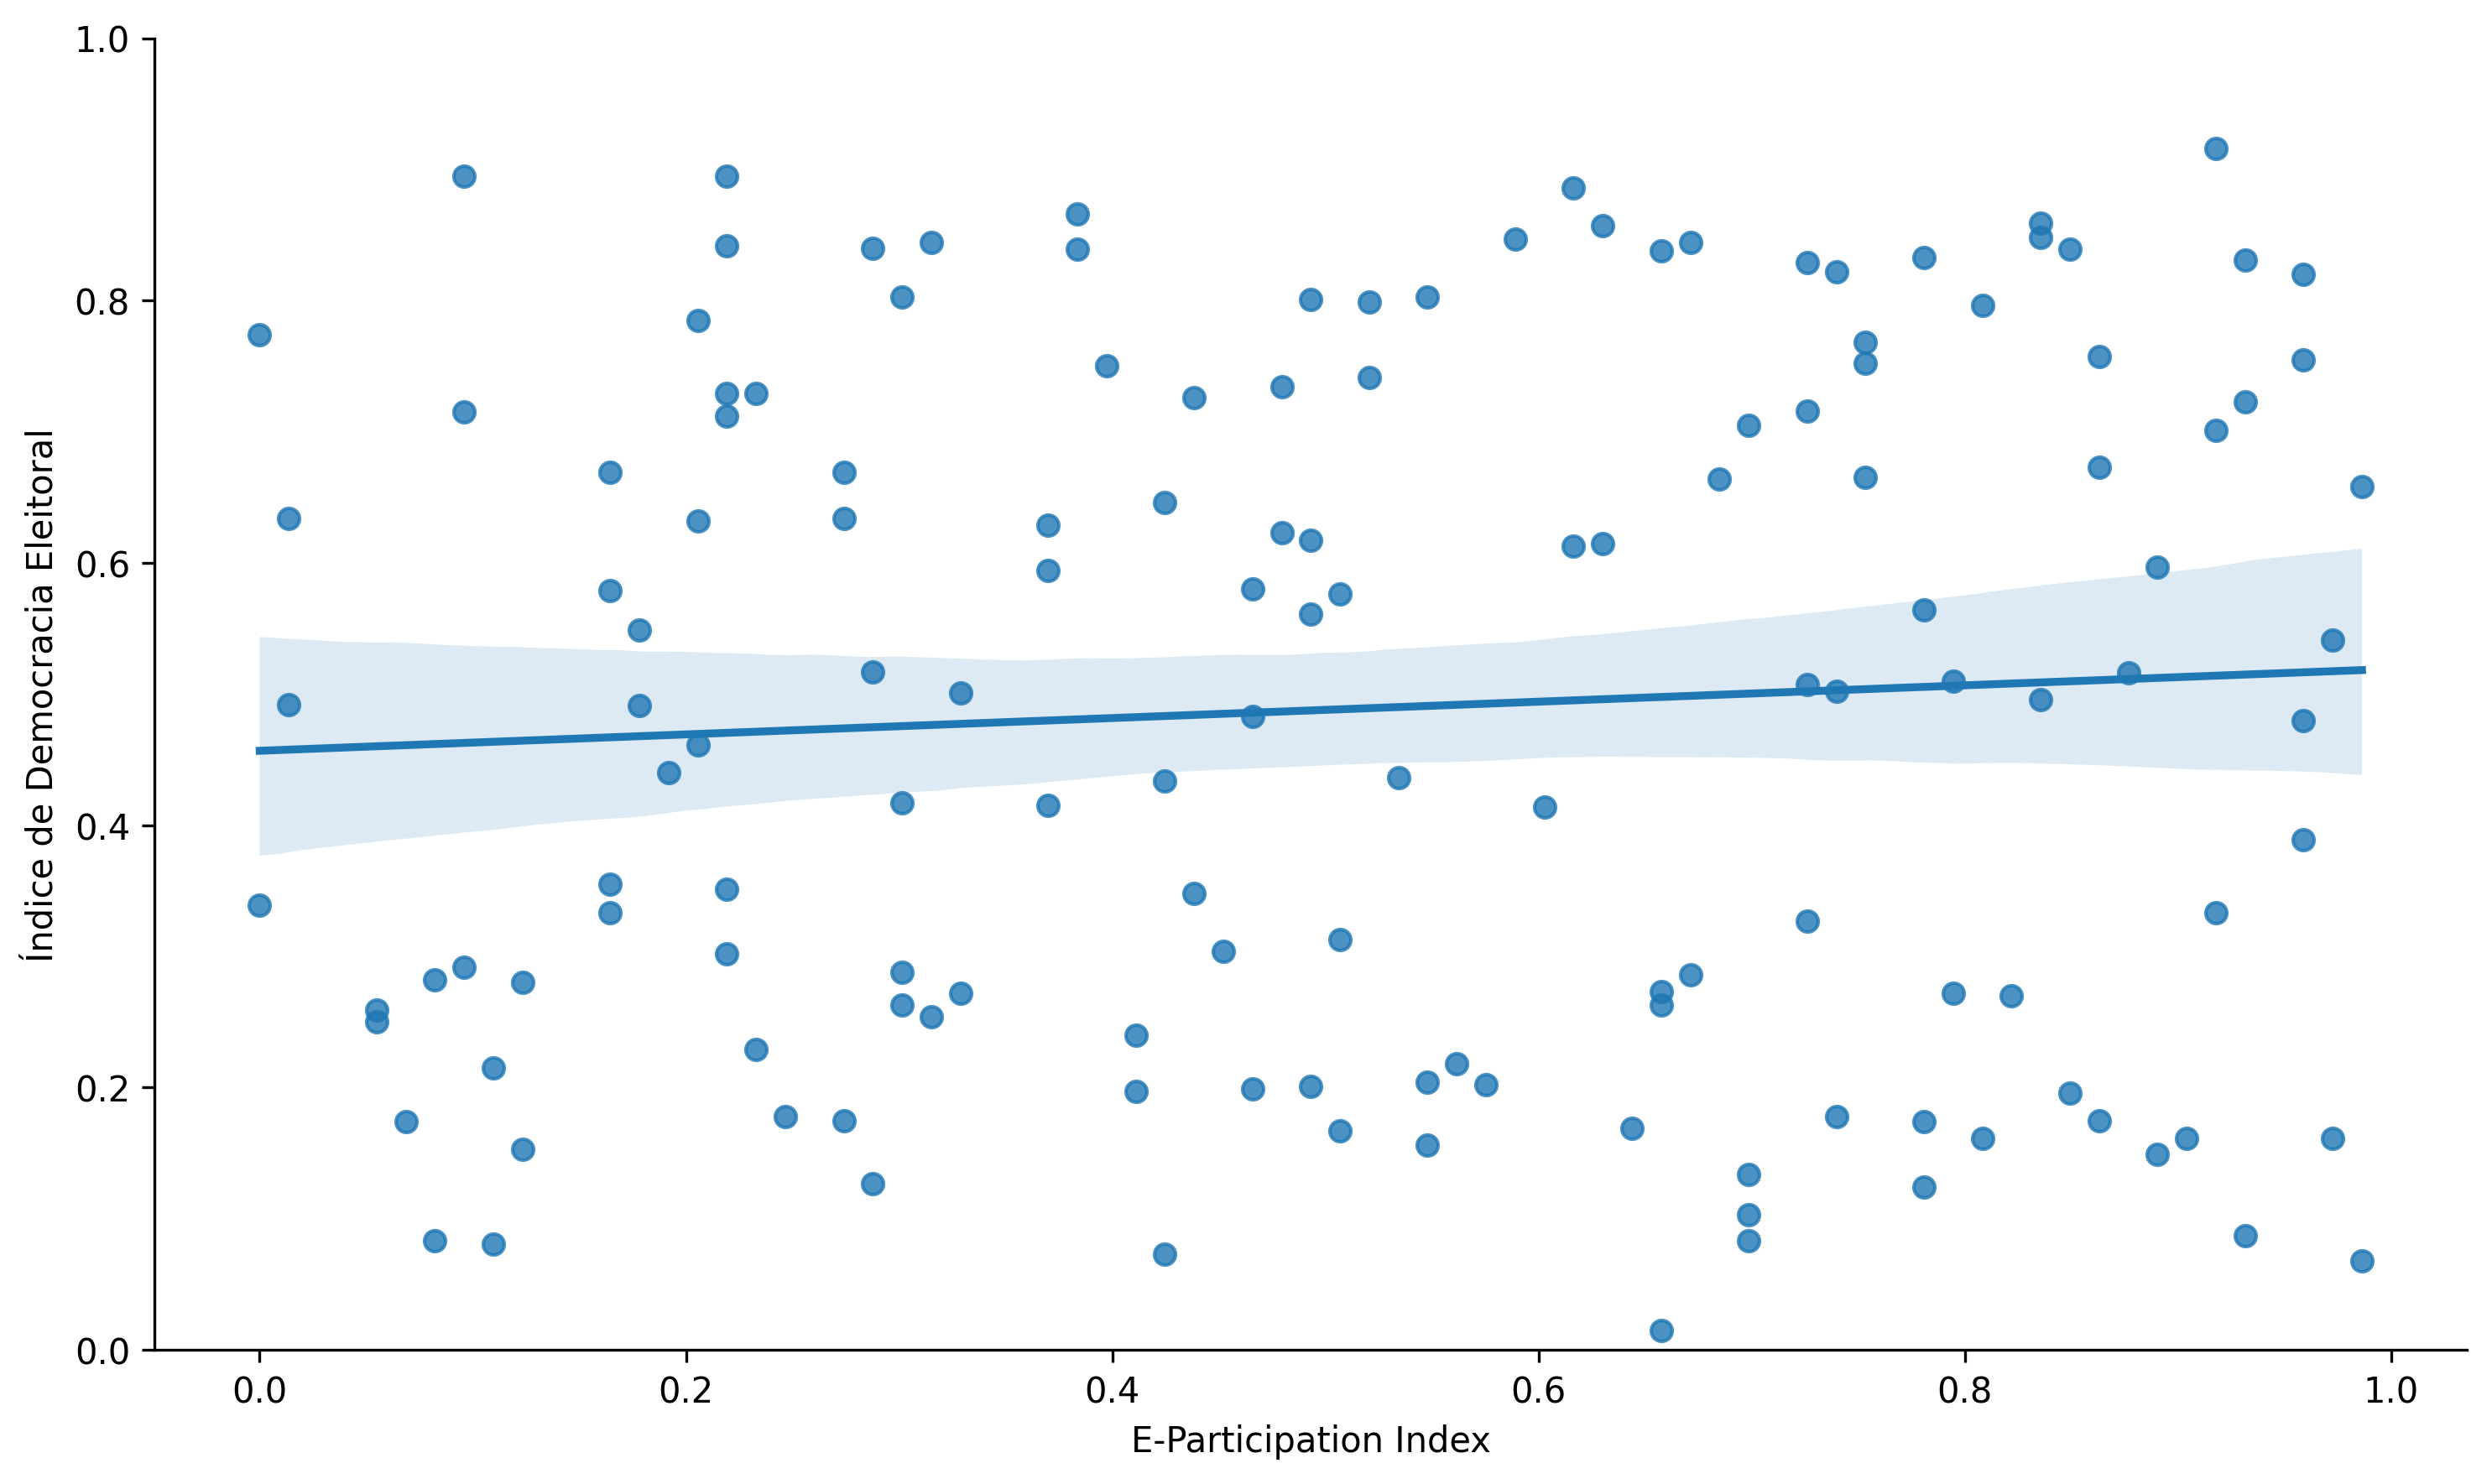
\includegraphics[width=1\linewidth]{figuras/egdi/dispersao_epart_indicedemocracia}
	\label{fig:dispersao_epart_indicedemocracia}
	\footnotesize{Fonte:baseado em \cite{ONU_EGDI_mapa} e \cite{electoral_democracy_index}}
\end{figure}

Para compreender melhor o diagrama de dispersão, foi usado o coeficiente de correlação de Spearman. A sua escolha foi motivada pela grande presença de pontos extremos. O coeficiente de correlação encontrada foi 0.05. Os índice de democracia eleitoral e o \textbf{E-Participation Index} são variáveis independentes.

\subsubsection{E-Government Development Index e gastos governamentais (\% do PIB)}

\begin{figure}[H]
	\centering
	\caption{Diagrama de Dispensao: E-Government Development Index e gastos governamentais (\% do PIB)}
	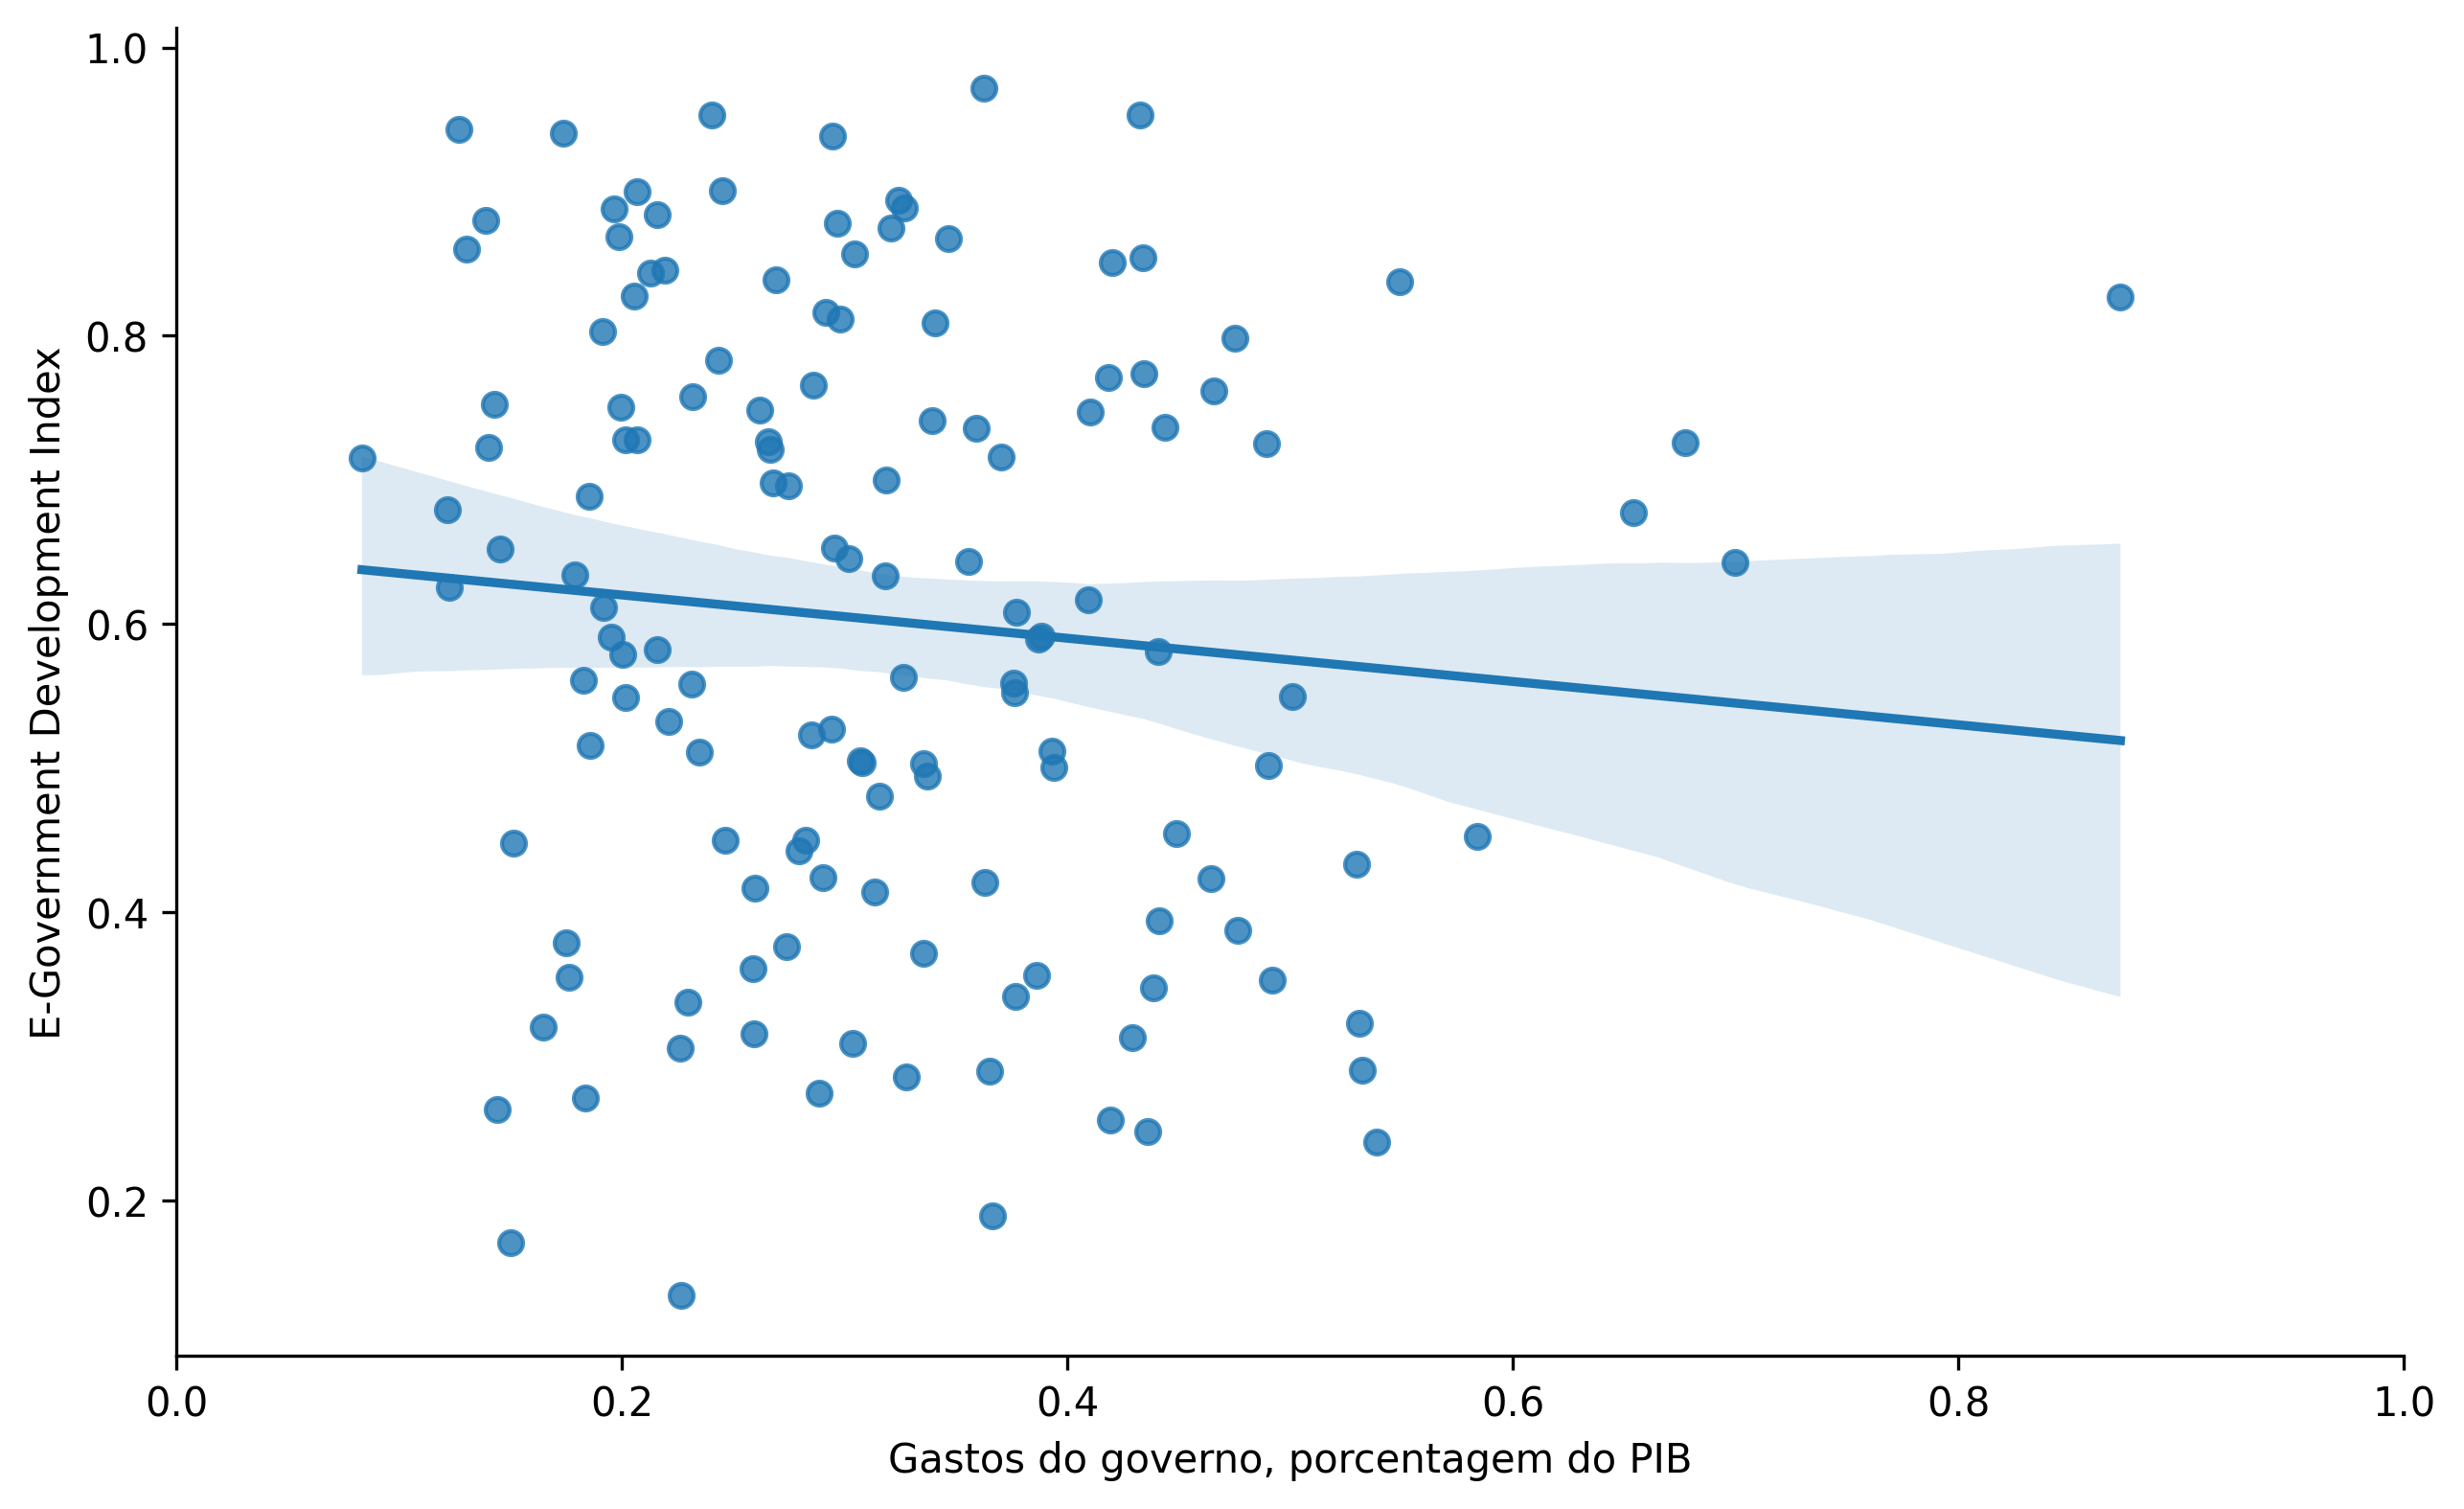
\includegraphics[width=1\linewidth]{figuras/egdi/dispersao_egov_govexpenditure}
	\label{fig:dispersao_egov_govexpenditure}
	\footnotesize{Fonte:baseado em \cite{ONU_EGDI_mapa} e \cite{FMI_gov_expenditure}}
\end{figure}

Para compreender melhor o diagrama de dispersão, foi usado o coeficiente de correlação de Spearman. A sua escolha foi motivada pela grande presença de pontos extremos. O coeficiente de correlação encontrada foi -0.13. O \textbf{E-Government Development Index} e os gastos públicos são variáveis independentes.

\subsubsection{E-Participation Index e gastos governamentais (\% do PIB)}

\begin{figure}[H]
	\centering
	\caption{Diagrama de Dispensao: E-Participation Index e gastos governamentais (\% do PIB)}
	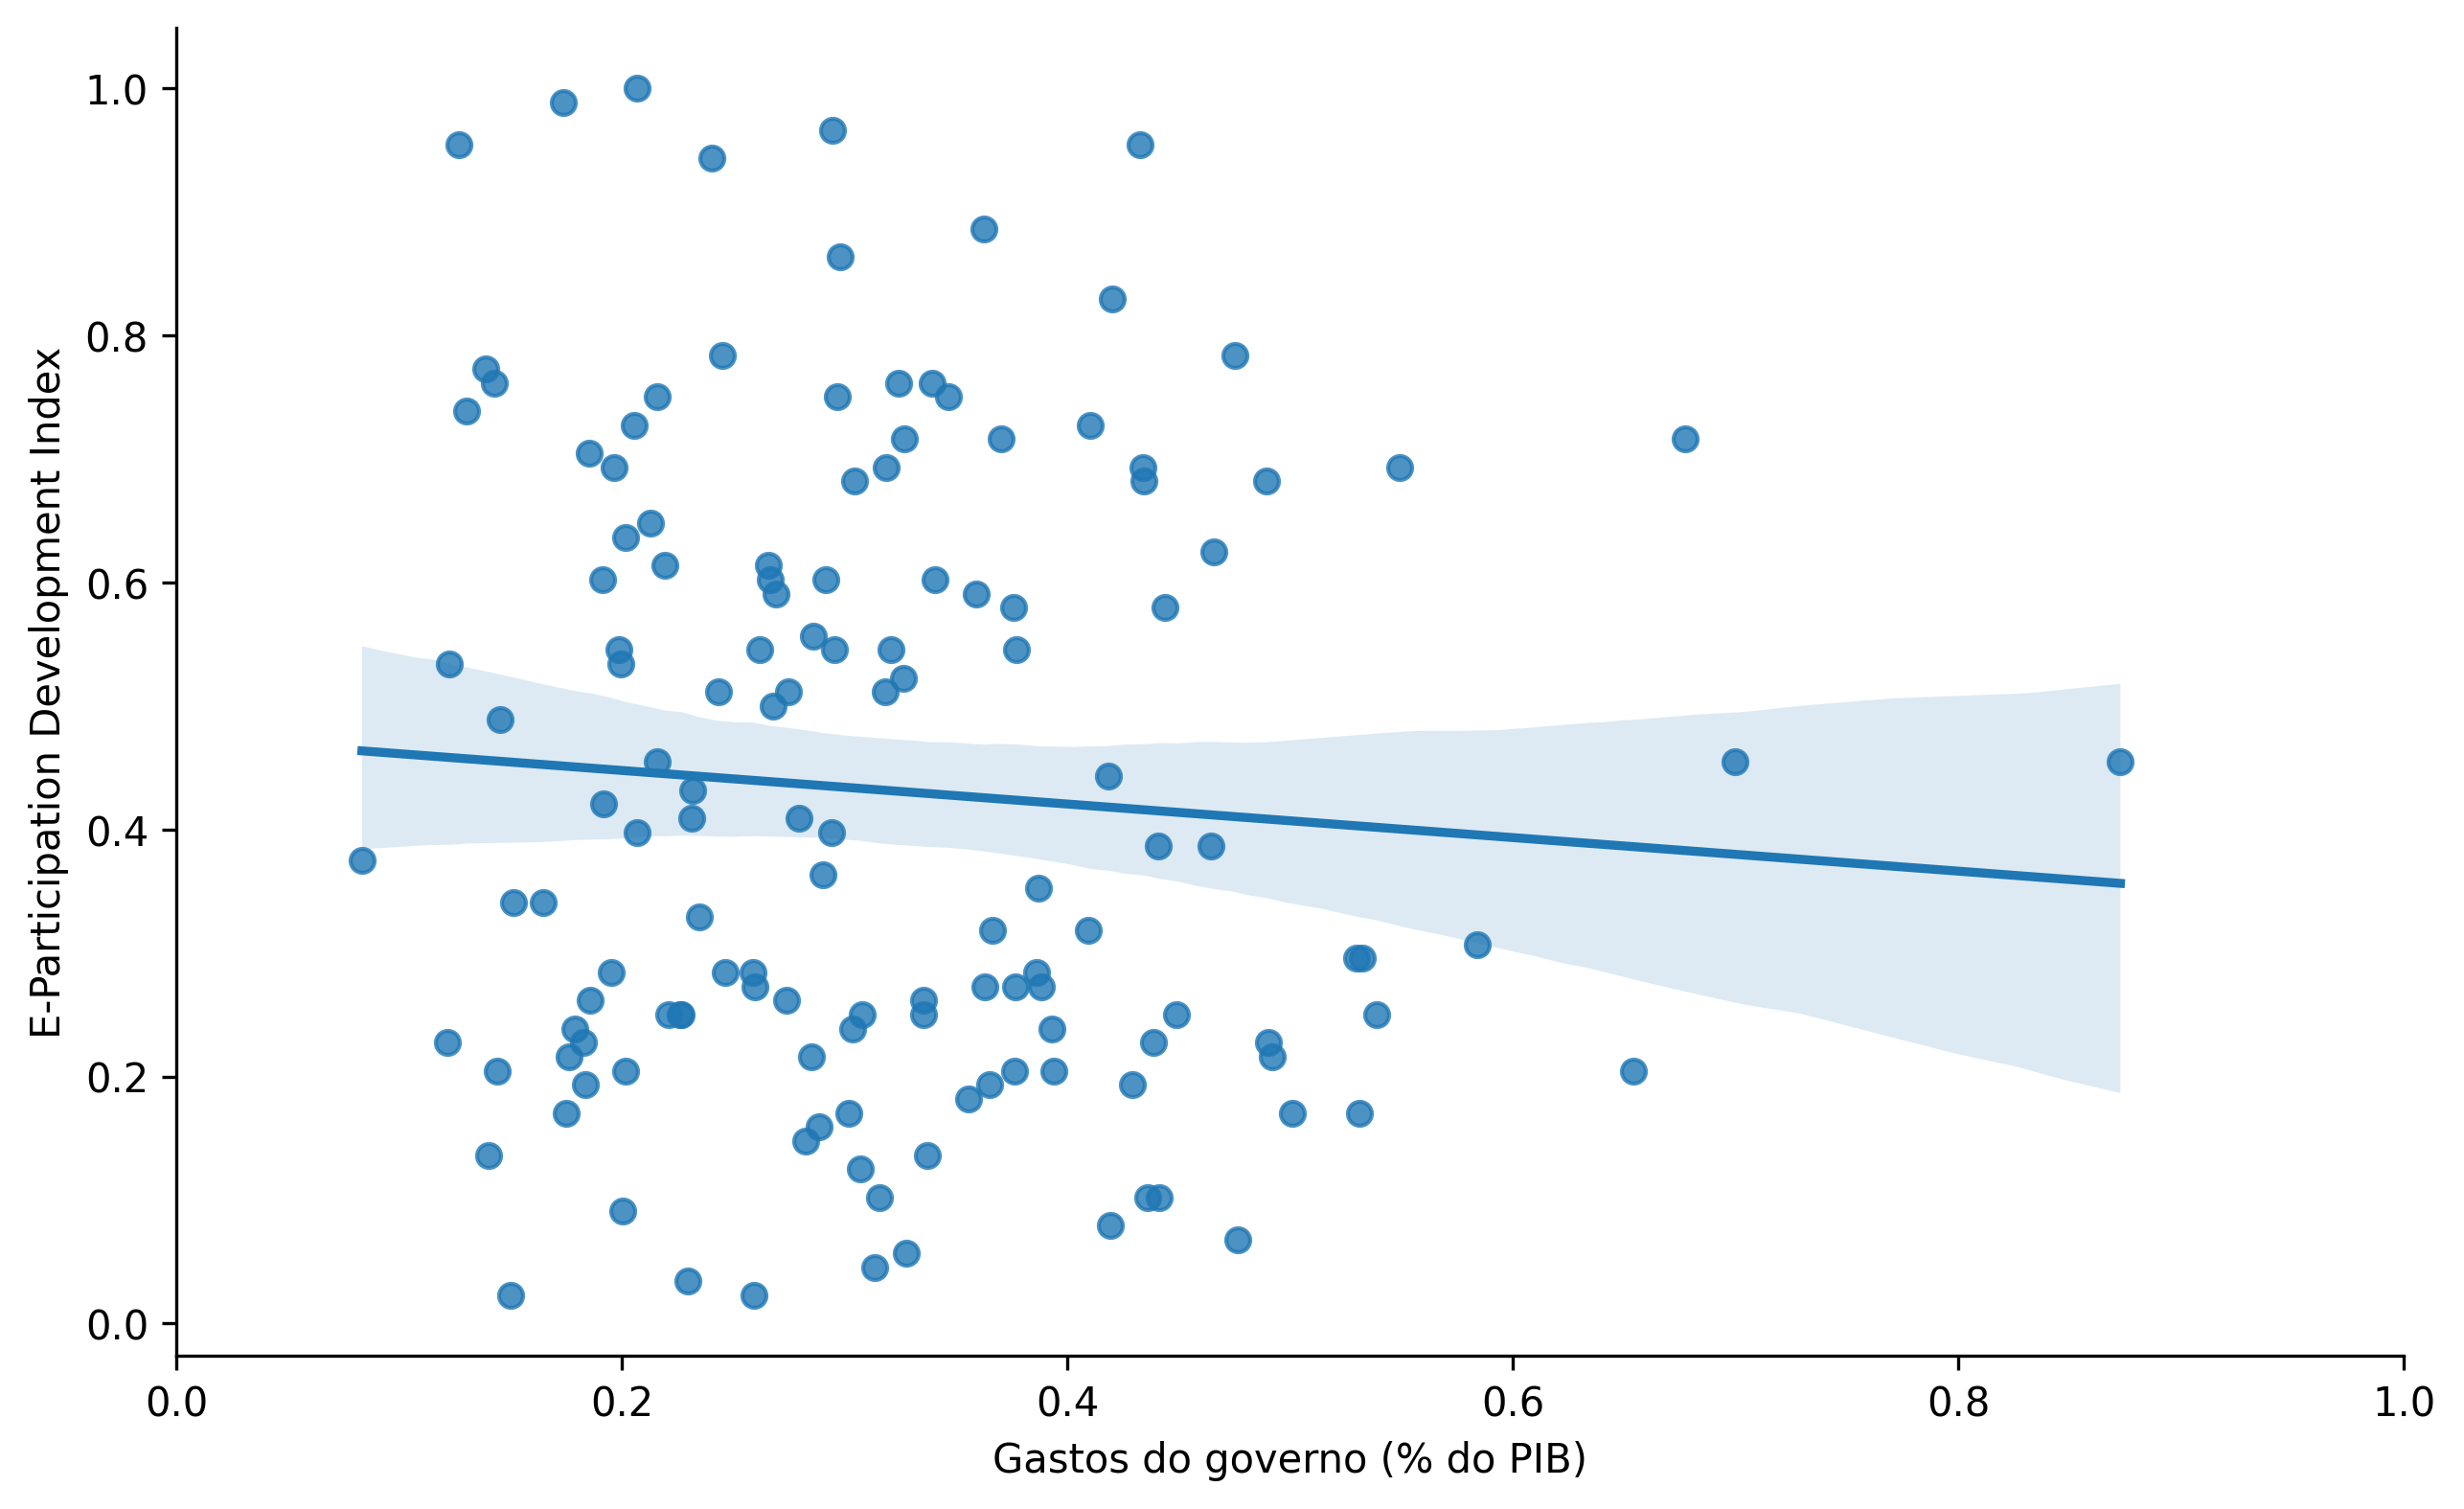
\includegraphics[width=1\linewidth]{figuras/egdi/dispersao_epart_govexpenditure}
	\label{fig:dispersao_epart_govexpenditure}
	\footnotesize{Fonte:baseado em \cite{ONU_EGDI_mapa} e \cite{FMI_gov_expenditure}}
\end{figure}

Para compreender melhor o diagrama de dispersão, foi usado o coeficiente de correlação de Spearman. A sua escolha foi motivada pela grande presença de pontos extremos. O coeficiente de correlação encontrada foi -0.07. O \textbf{E-Participation Index} e os gastos públicos são variáveis independentes.

\subsection{Análise granular com os componentes do EGDI}

\subsubsection{PIB \textit{per capita} PPC}

\subsubsection{PIB \textit{per capita} PPC}

\subsubsection{PIB \textit{per capita} PPC}

\subsubsection{índice de democracia eleitoral}

\subsubsection{índice de democracia eleitoral}

\subsubsection{índice de democracia eleitoral}

\subsubsection{gastos governamentais (\% do PIB)}

\subsubsection{gastos governamentais (\% do PIB)}

\subsubsection{gastos governamentais (\% do PIB)}



\section{Indicadores de TIC de governo eletrônico}
\label{indicadores_tic_egov}

A ONU tem \href{https://publicadministration.un.org/egovkb/en-us/Data/ICT-in-government}{indicadores de TIC de governo eletrônico} como algo complementar ao EGDI. Os indicadores são, conforme \cite{ONU_ICT_in_government_indicators}:

\begin{itemize}
	\item Existência de estratégia nacional de governo eletrônico ou equivalente;
	\item Existência de identidade digital para acessar ou outra forma de autenticação requirida para poder acessar serviços online;
	\item Existência de um portal de compras governamentais.
\end{itemize}

Os resultados globais dos indicadores estão presentes nas figuras \ref{fig:national_government_strategy}, \ref{fig:national_identity} e \ref{fig:procurement_portal}.

\begin{figure}[H]
	\centering
	\caption{Indicador: Existência de estratégia nacional de governo eletrônico ou equivalente}
	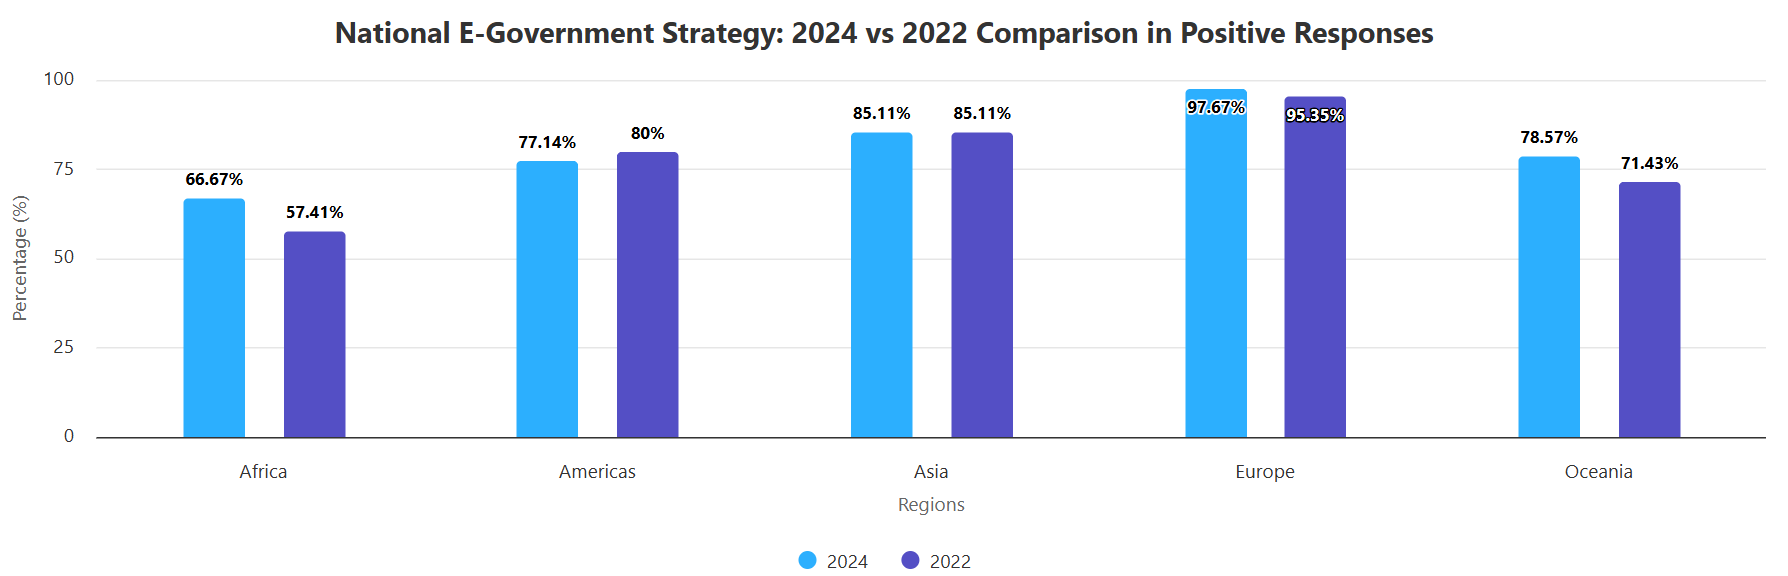
\includegraphics[width=1\linewidth]{figuras/ict_in_government/national_government_strategy}
	\label{fig:national_government_strategy}
	\footnotesize{Fonte: \cite{ONU_ICT_in_government_indicators}}
\end{figure}

\begin{figure}[H]
	\centering
	\caption{Indicador: Existência de identidade digital para acessar ou outra forma de autenticação requirida para poder acessar serviços online}
	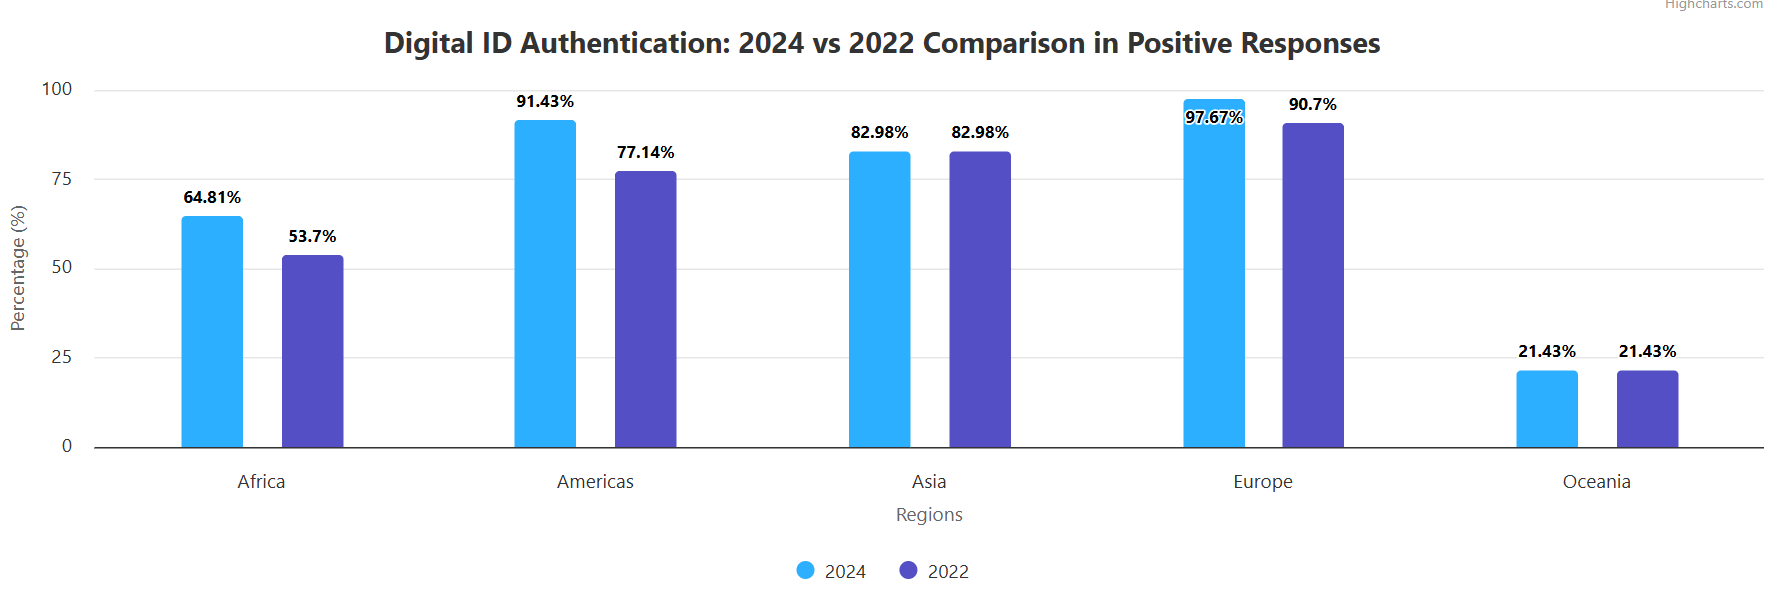
\includegraphics[width=1\linewidth]{figuras/ict_in_government/digital_identity}
	\label{fig:national_identity}
	\footnotesize{Fonte: \cite{ONU_ICT_in_government_indicators}}
\end{figure}

\begin{figure}[H]
	\centering
	\caption{Indicador: Existência de um portal de compras governamentais}
	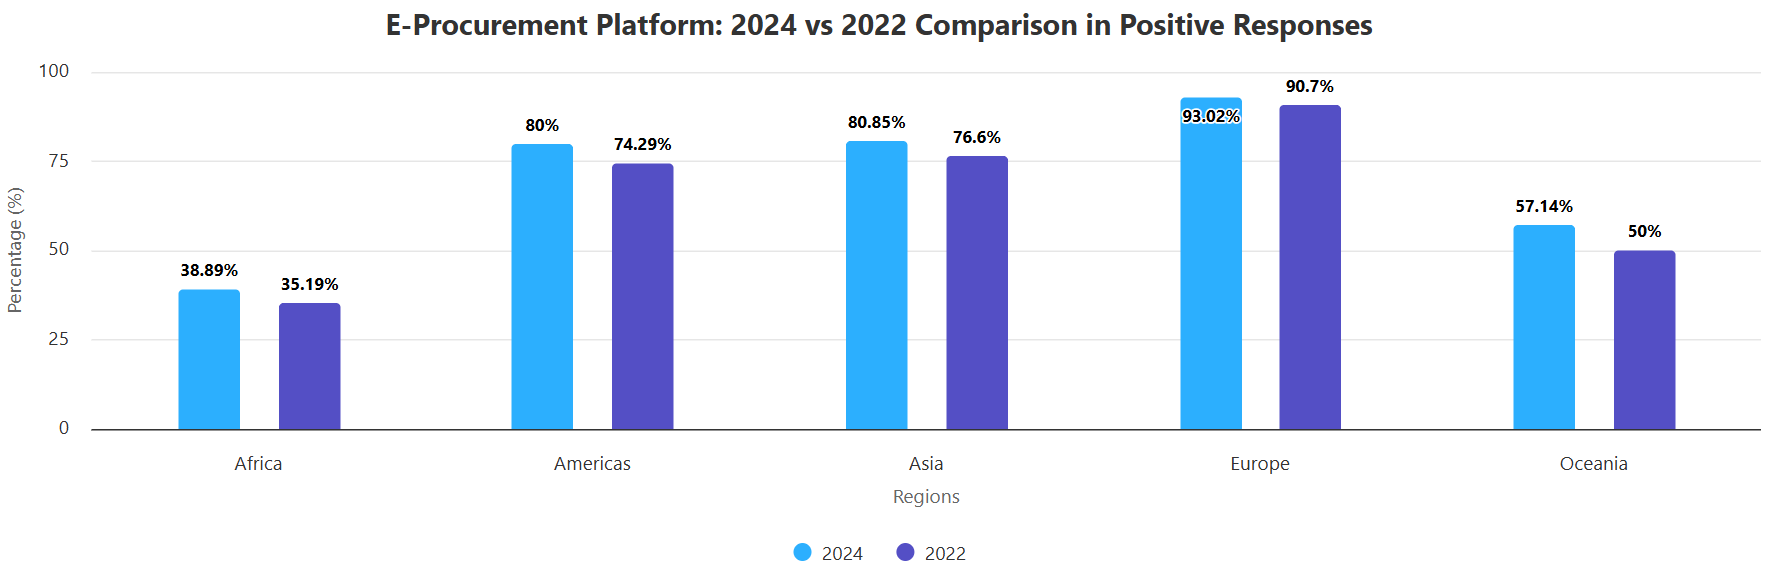
\includegraphics[width=1\linewidth]{figuras/ict_in_government/procurement_portal}
	\label{fig:procurement_portal}
	\footnotesize{Fonte: \cite{ONU_ICT_in_government_indicators}}
\end{figure}

Extraí-se das três figuras que a Europa foi o continente cujos mais respondem que têm seguem os indicadores, superando os 90\%. A Oceania foi o continente que menos implementou políticas de identidade digital para acesso a serviços online. África e Oceania tiveram um desempenho ruim na implementação de portais de compra governamentais. O continente americano apresentou bom desempenho nos três indicadores.

Como consequência da análise dos resultados presentes nas figuras \ref{fig:national_government_strategy}, \ref{fig:national_identity} e \ref{fig:procurement_portal}, buscou-se entender a seguinte situação registrada nos 2022 e 2024, anos em que os indicadores foram medidos: qual é a porcentagem de países que responderam nenhuma, uma, duas ou todas as perguntas. Elas usam sim ou não para confirmar a aplicação dos indicadores no país.

A resposta ao questionamento está presente na figura \ref{fig:indicators_answer}.

\begin{figure}[H]
	\centering
	\caption{Respostas positivas aos indicadores de TIC de governo eletrônico}
	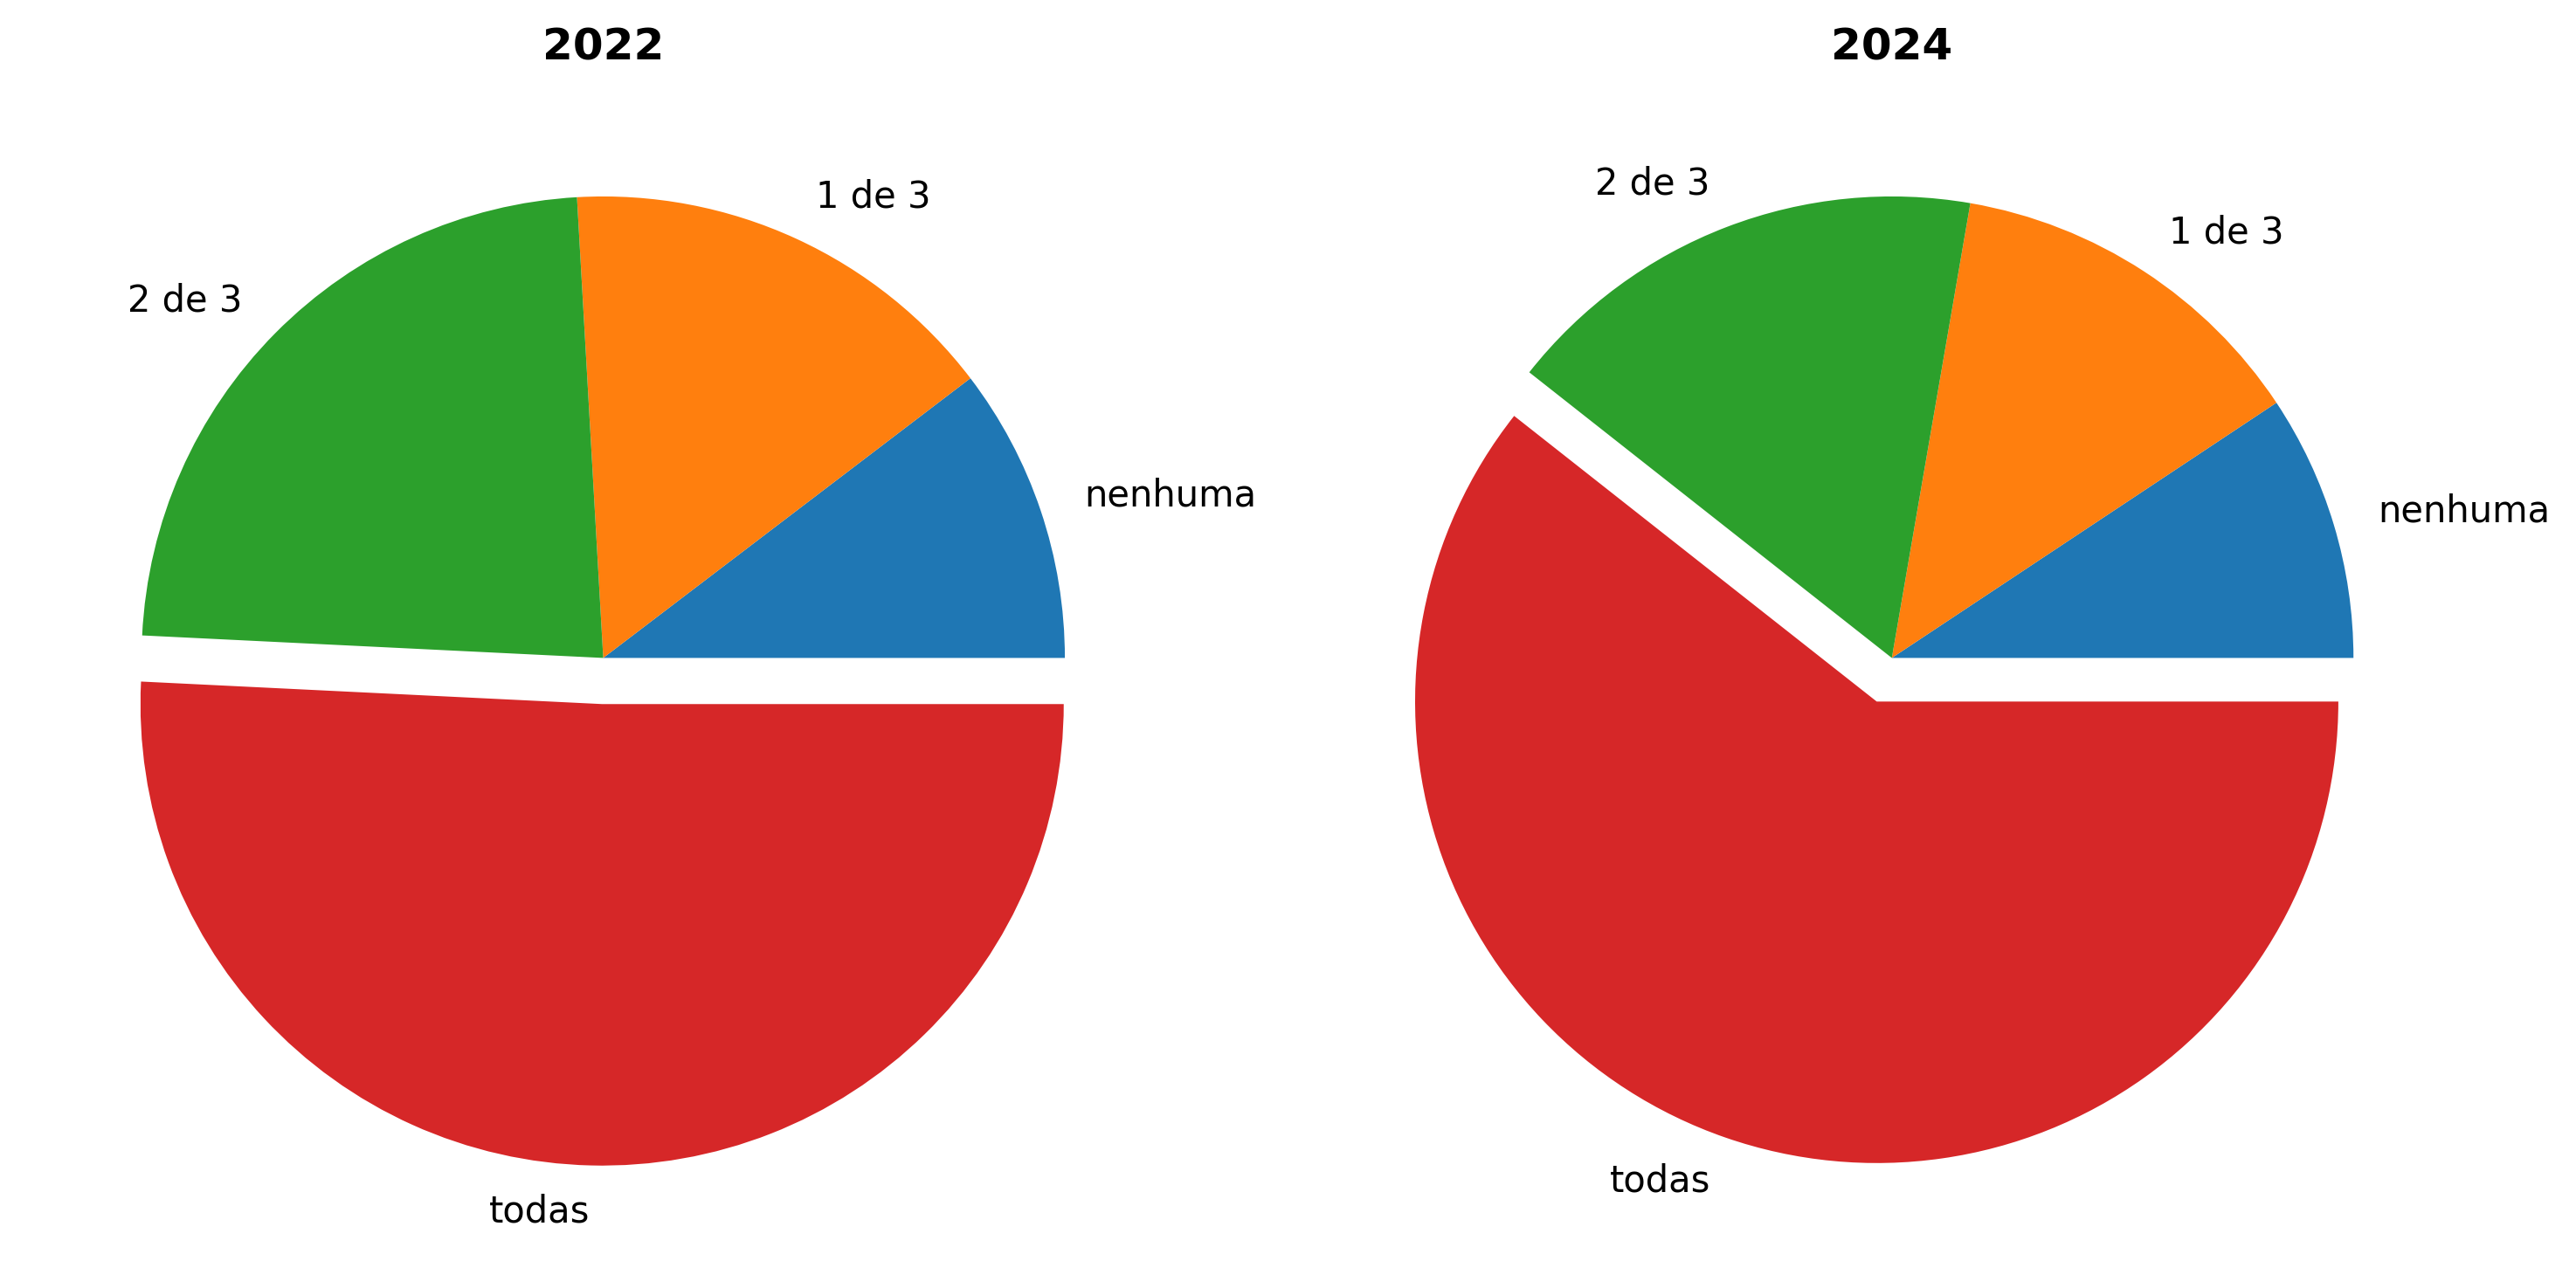
\includegraphics[width=1\linewidth]{figuras/ict_in_government/indicators_answer}
	\label{fig:indicators_answer}
	\footnotesize{Fonte: \cite{ONU_ICT_in_government_indicators}}
\end{figure}

Em 2022, metade dos países respondeu positivamente as três perguntas; em 2024, mais da metade. O Brasil faz parte desse grupo, tal como a Rússia e China. A mudança é creditada a redução do número de países que responderam positivamente 2 de 3 perguntas e passaram a responder as três positivamente. 

Além, disso a quantidade de países que responderam positivamente 1 de 3 perguntas e nenhuma se igualou em 2024, sendo os países que responderam 1 de 3 perguntas era maior do que os que responderam nenhuma.

\section{Coeficiente de correlação: indicadores de TIC de governo eletrônico comparados com outras variáveis}

Com base na seção \ref{indicadores_tic_egov}, buscou-se entender se há correlação entre os indicadores de TIC de governo eletrônico e os PIB \textit{per capita} PPC e índice de democracia eleitoral.

\begin{figure}[H]
	\centering
	\caption{Diagrama de Dispersão: indicadores de TIC de governo eletrônico e PIB \textit{per capita} PPC}
	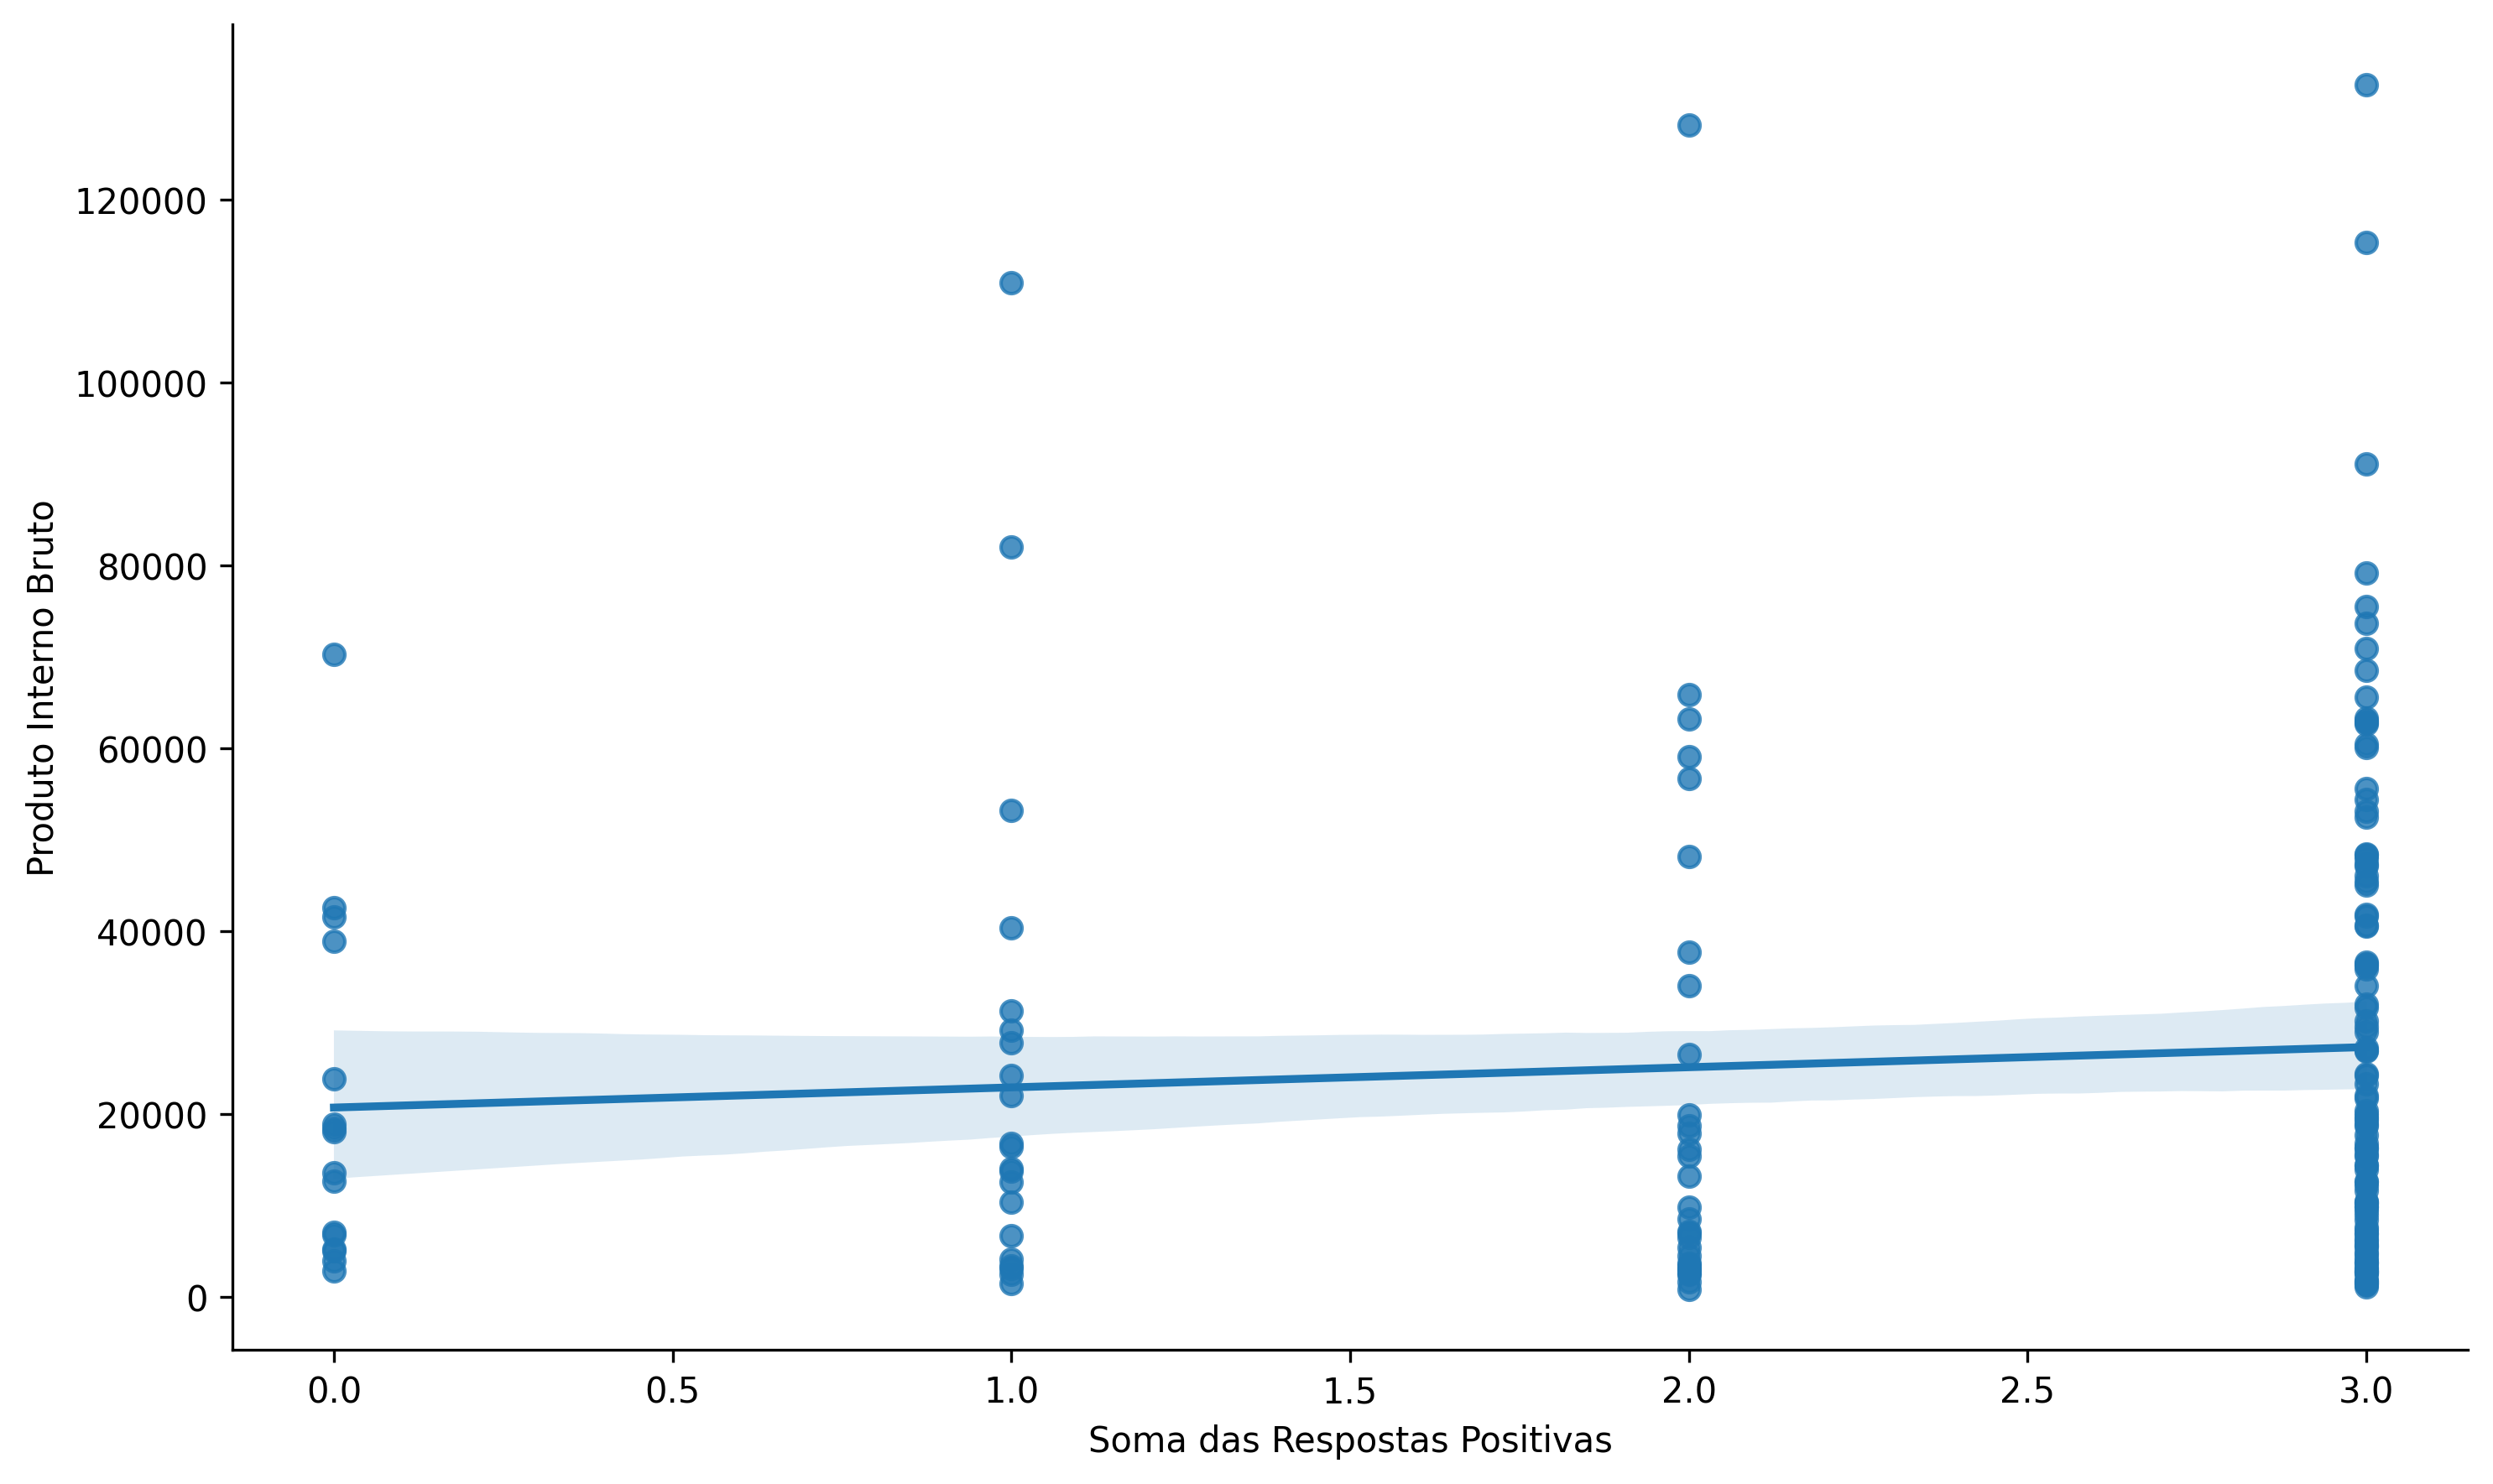
\includegraphics[width=1\linewidth]{figuras/ict_in_government/dispersao_ticegov_pib}
	\label{fig:dispersao_ticegov_pib}
	\footnotesize{Fonte: baseado em \cite{WB_pib_per_capita_países} e \cite{ONU_ICT_in_government_indicators}}
\end{figure}

\begin{figure}[H]
	\centering
	\caption{Diagrama de Dispersão: indicadores de TIC de governo eletrônico e índice de democracia eleitoral}
	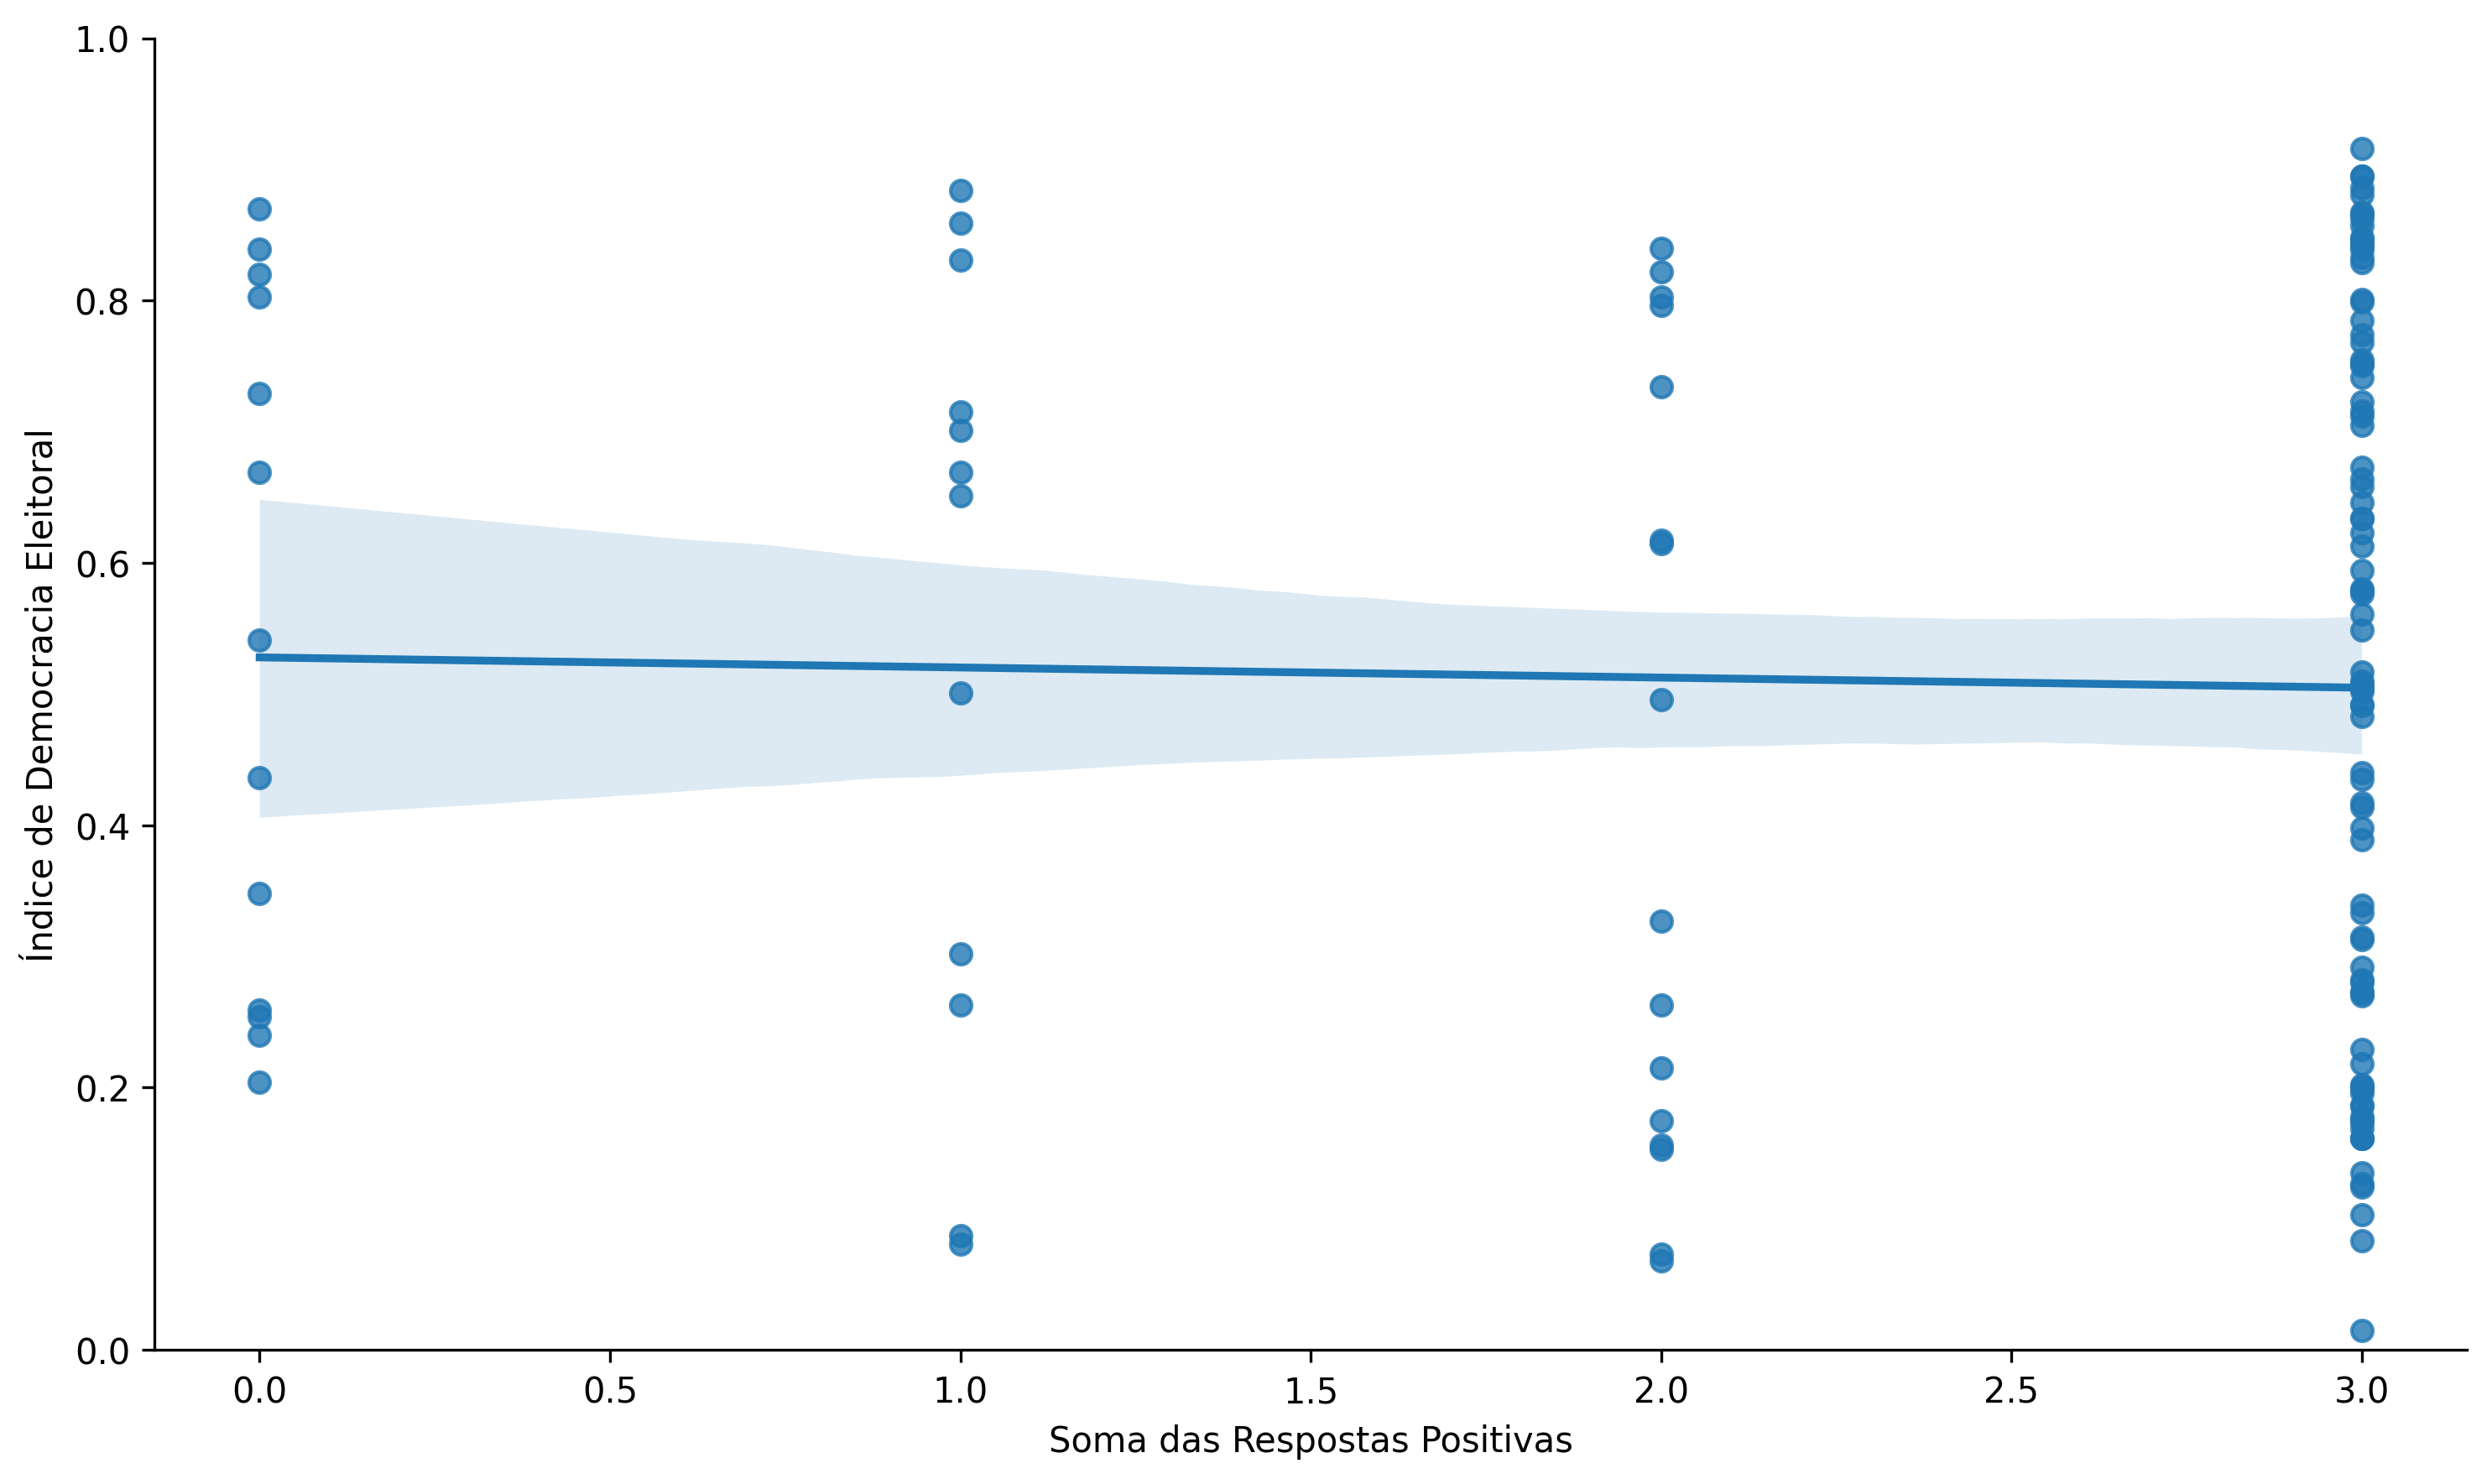
\includegraphics[width=1\linewidth]{figuras/ict_in_government/dispersao_ticegov_indicedemocracia}
	\label{fig:dispersao_ticegov_indicedemocracia}
	\footnotesize{Fonte: baseado em \cite{electoral_democracy_index} e \cite{ONU_ICT_in_government_indicators}}
\end{figure}

Como os diagramas de dispersão presentes nas figuras \ref{fig:dispersao_ticegov_pib} e \ref{fig:dispersao_ticegov_indicedemocracia}  apresentaram grande dispersão em relação à tendência, optou-se pelo uso do coeficiente de correlação de Spearman. A alta dispersão em relação à tendência é um indicativo de um coeficiente de correlação neutro ou baixo. Os coeficientes de correlação (0.1 e -0.0051) indicam que os indicadores de TIC de governo eletrônico não são afetados pelo PIB per capita PPC e pelo índice de democracia eleitoral, e vice-versa.

Outra análise feita foi a comparação entre os indicadores de TIC de governo eletrônico e os gastos governamentais.

\begin{figure}[H]
	\centering
	\caption{Diagrama de Dispersão: indicadores de TIC de governo eletrônico e gastos governamentais (\% do PIB)}
	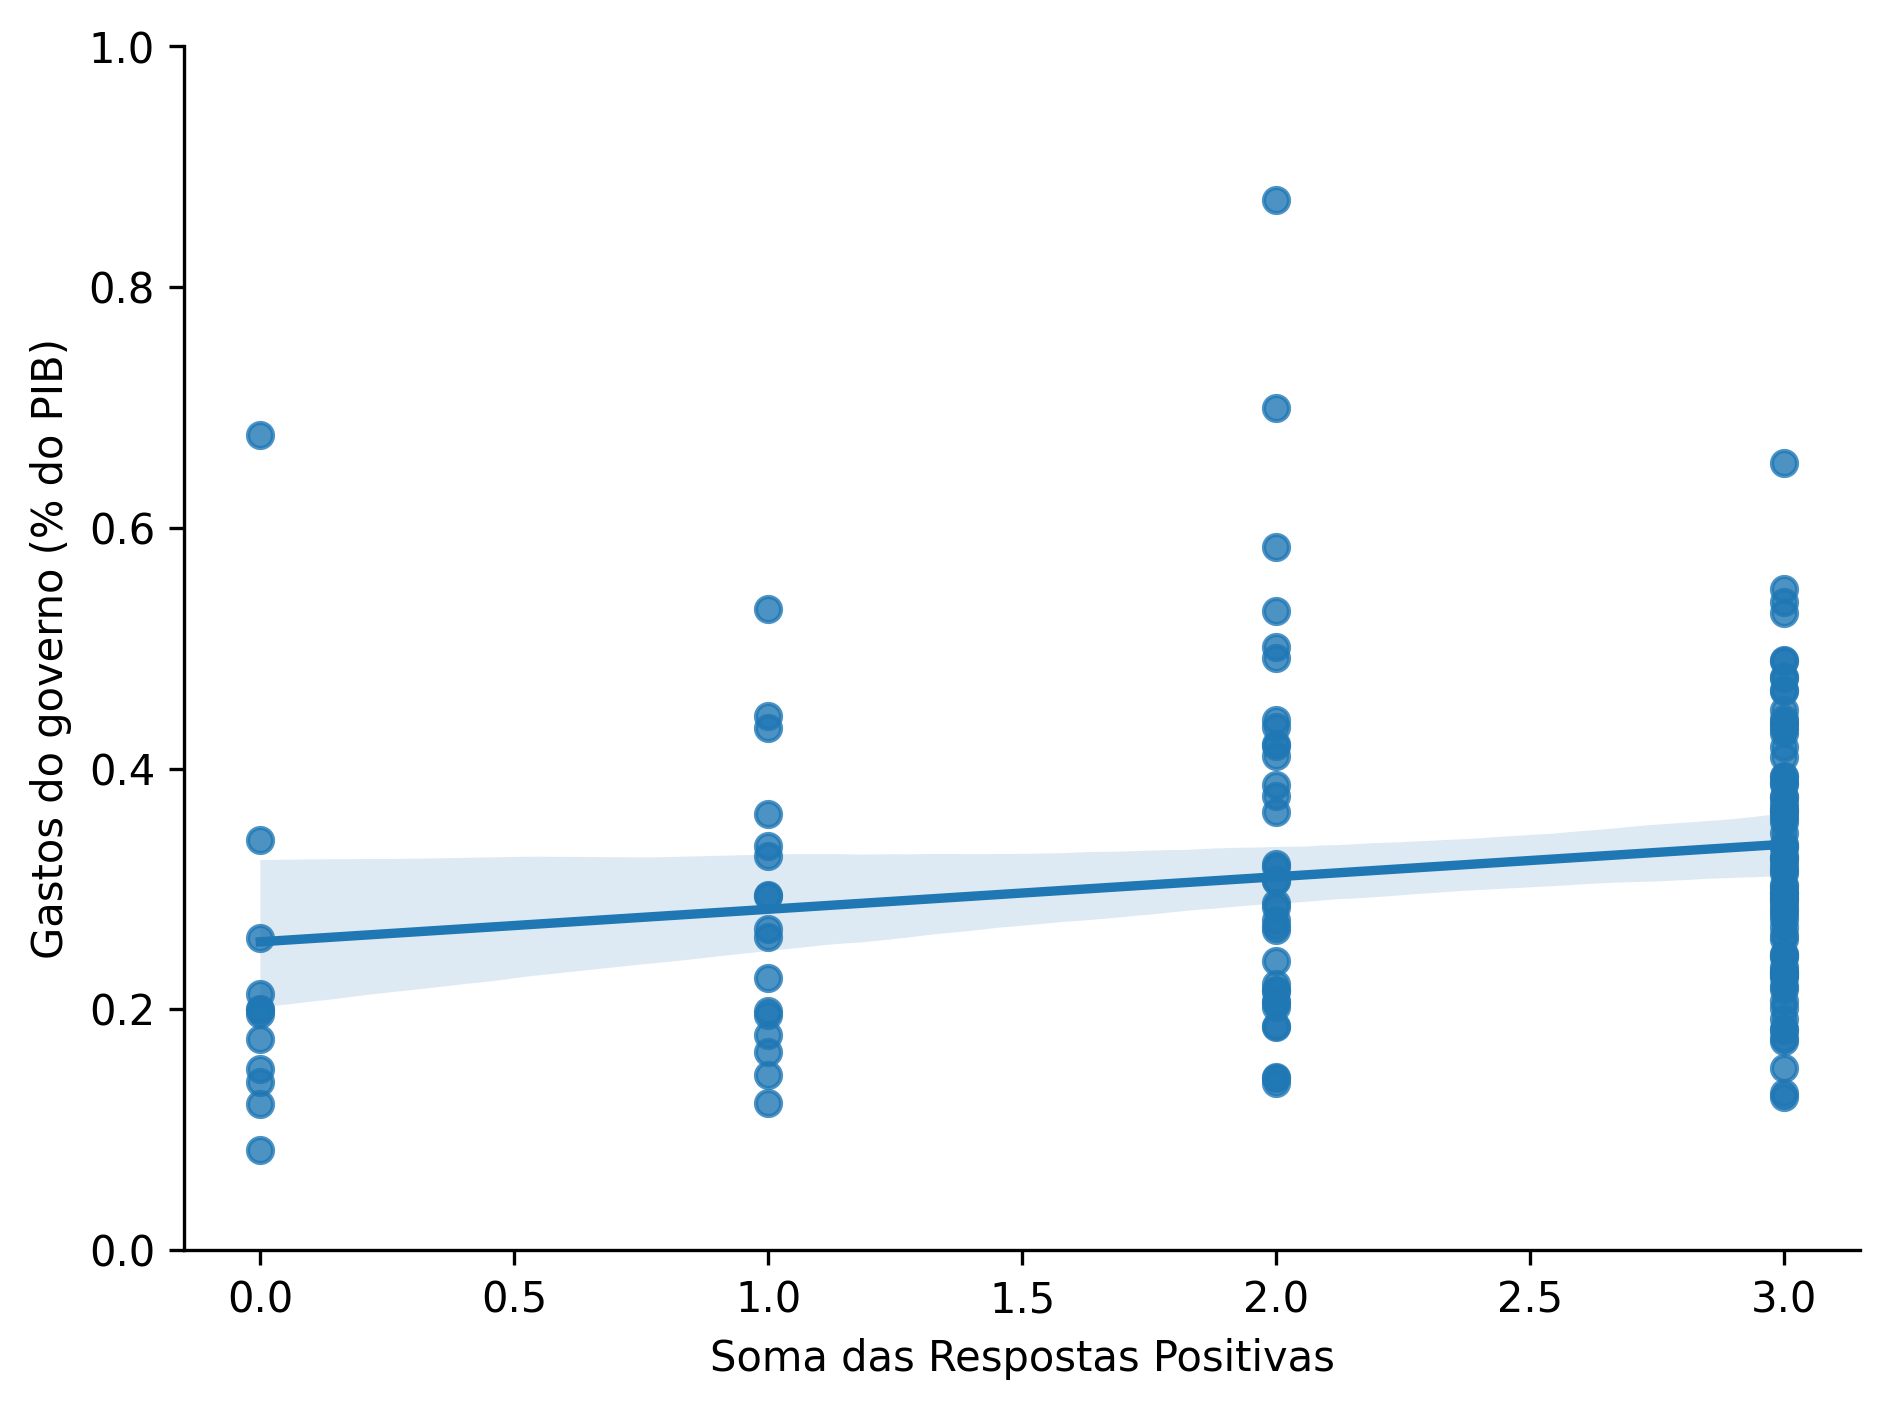
\includegraphics[width=1\linewidth]{figuras/egdi/dispersao_ticegov_govexpenditure}
	\label{fig:dispersao_ticegov_govexpenditure}
	\footnotesize{Fonte: baseado em \cite{FMI_gov_expenditure} e \cite{ONU_ICT_in_government_indicators}}
\end{figure}

Para compreender melhor o diagrama de dispersão, foi usado o coeficiente de correlação de Spearman. A sua escolha foi motivada pela grande presença de pontos extremos. O coeficiente de correlação encontrada foi 0.23. O referido coeficiente indica uma correlação positiva muito fraca entre os gastos do governo e a soma das respostas positivas. 


\section{Dados do Brasil}

A figura \ref{fig:lineplot_egdi_brasil} mostra evolução do EGDI do Brasil desde 2003-2005 e 2008-2024 (bianualmente).

\begin{figure}[H]
	\centering
	\caption{Evolução do EGDI do Brasil (2003-2005, 2008-2024 bianualmente)}
	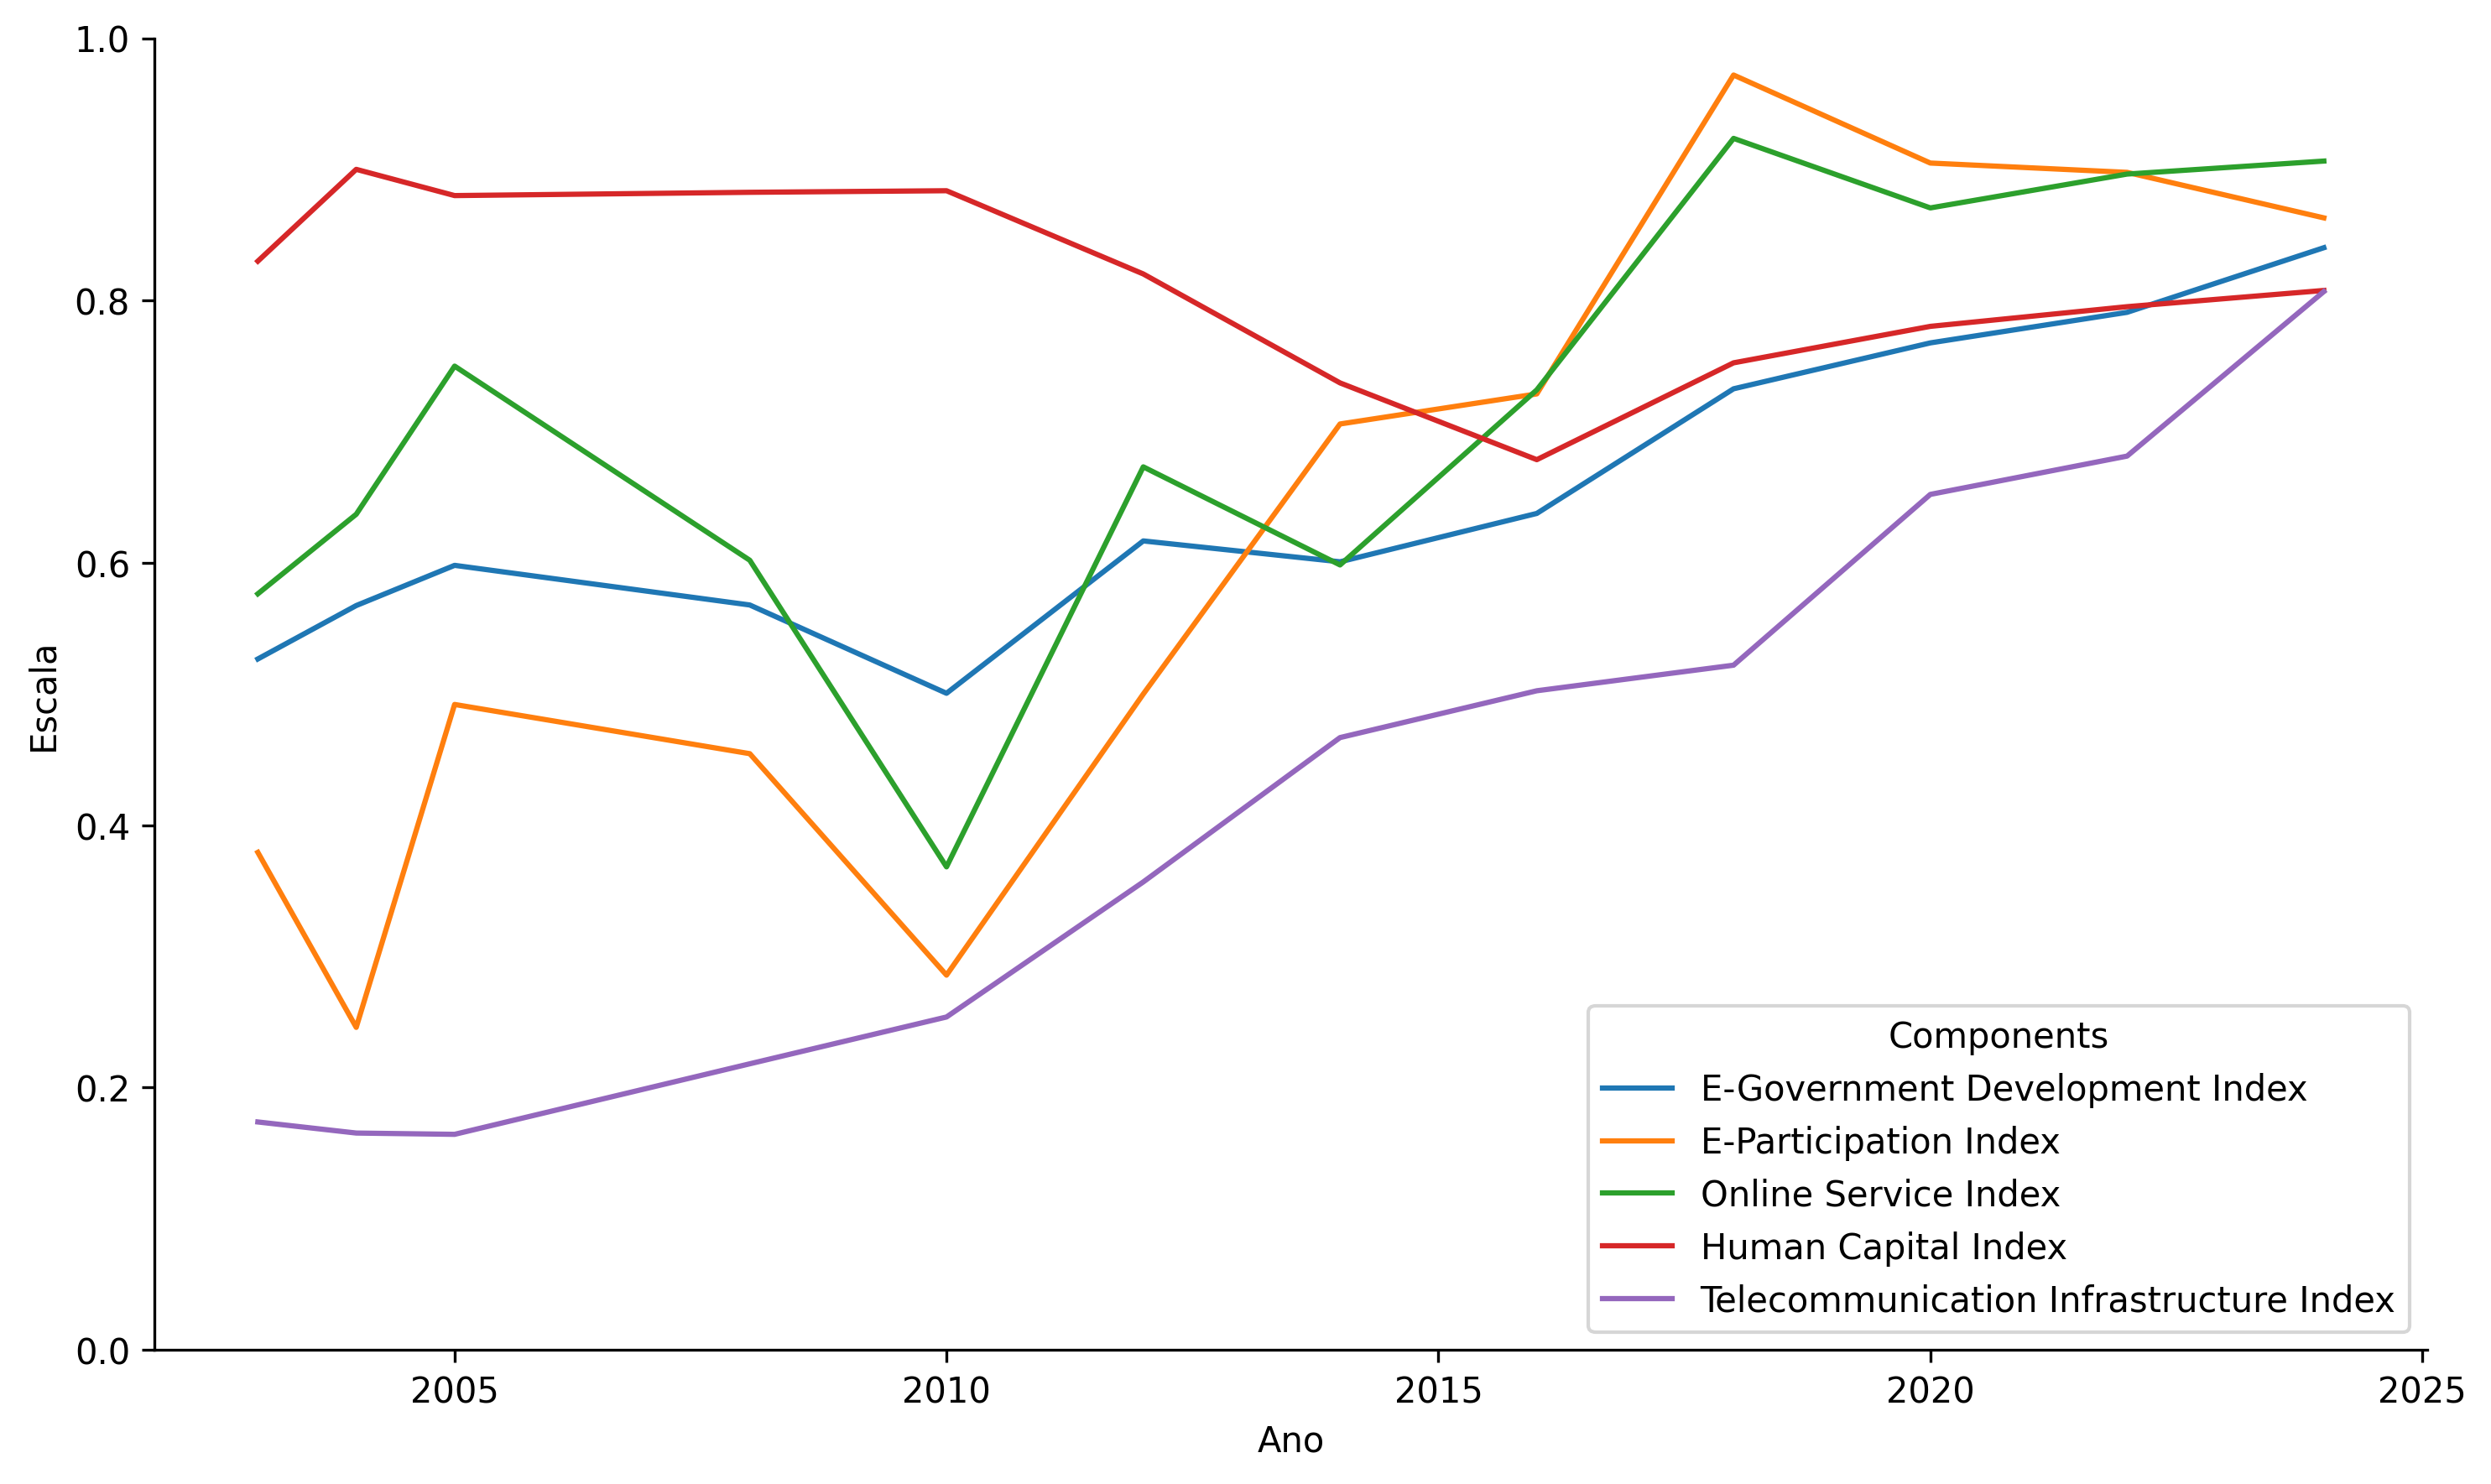
\includegraphics[width=1\linewidth]{figuras/egdi/lineplot_egdi_brasil.png}
	\label{fig:lineplot_egdi_brasil}
	\footnotesize{Fonte: baseado em \cite{ONU_EGDI_mapa}.}
\end{figure}

A maioria dos índices (\textbf{E-Government Development}, \textbf{Online Service},  \textbf{Human Capital} e, especialmente, o de  \textbf{Telecommunications Infrastructure}) apresenta uma tendência geral de crescimento ao longo do período, indicando uma melhoria na digitalização do governo e da sociedade brasileira.

Os  \textbf{E-Participation Index} e o \textbf{Online Service Index} mostram as maiores flutuações, com picos e quedas significativas em diferentes anos. Isso pode indicar variações nas políticas ou na implementação de serviços digitais e na participação cidadã.

\subsubsection{E-Government Development Index} O índice principal mostra um crescimento constante, mas gradual, partindo de cerca de 0.5 em 2003 e atingindo mais de 0.8 em 2024. Sua trajetória reflete a média dos outros componentes, indicando uma evolução geral da capacidade do governo de fornecer serviços online.

\subsubsection{E-Participation Index} Este índice é o mais volátil e o que apresenta o menor desempenho em grande parte do período. Ele tem um pico notável em 2005, seguido de uma queda e uma lenta recuperação. Isso sugere que a participação cidadã por meio de canais digitais é uma área que enfrenta desafios e flutuações, e seu desenvolvimento pode não ser tão linear quanto o de outros componentes.

\subsubsection{Online Service Index} Após um pico inicial, este índice apresenta uma queda acentuada por volta de 2010, seguido de uma recuperação e um novo pico em 2018. Sua trajetória é irregular, o que pode refletir desafios na oferta de serviços públicos online. No entanto, ele termina o período em um nível alto, próximo do Human Capital Index.

\subsubsection{Human Capital Index} Este índice mantém um nível consistentemente alto, geralmente entre 0.8 e 0.9, sendo o que mais se aproxima do valor máximo da escala. Apesar de algumas flutuações, ele demonstra que o Brasil possui um bom nível de capital humano para suportar o desenvolvimento do e-government, como educação e alfabetização digital.

\subsubsection{Telecommunication Infrastructure Index} Este é o índice com o crescimento mais notável e constante. Ele parte de um patamar baixo (abaixo de 0.2 em 2003) e alcança o maior valor entre todos os índices no final do período (próximo de 0.8 em 2024). Isso sugere um avanço significativo na infraestrutura digital do país, como a expansão de banda larga e redes de telecomunicações.

\subsection{Comparando as métricas do Brasil com a média internacional de 2024}

A figura \ref{fig:barplot_egdi_mediamundial_brasil} contém os valores do EGDI e seus componentes do Brasil e da média mundial de 2024.

\begin{figure}[H]
	\centering
	\caption{EGDI do Brasil e a média mundial em 2024}
	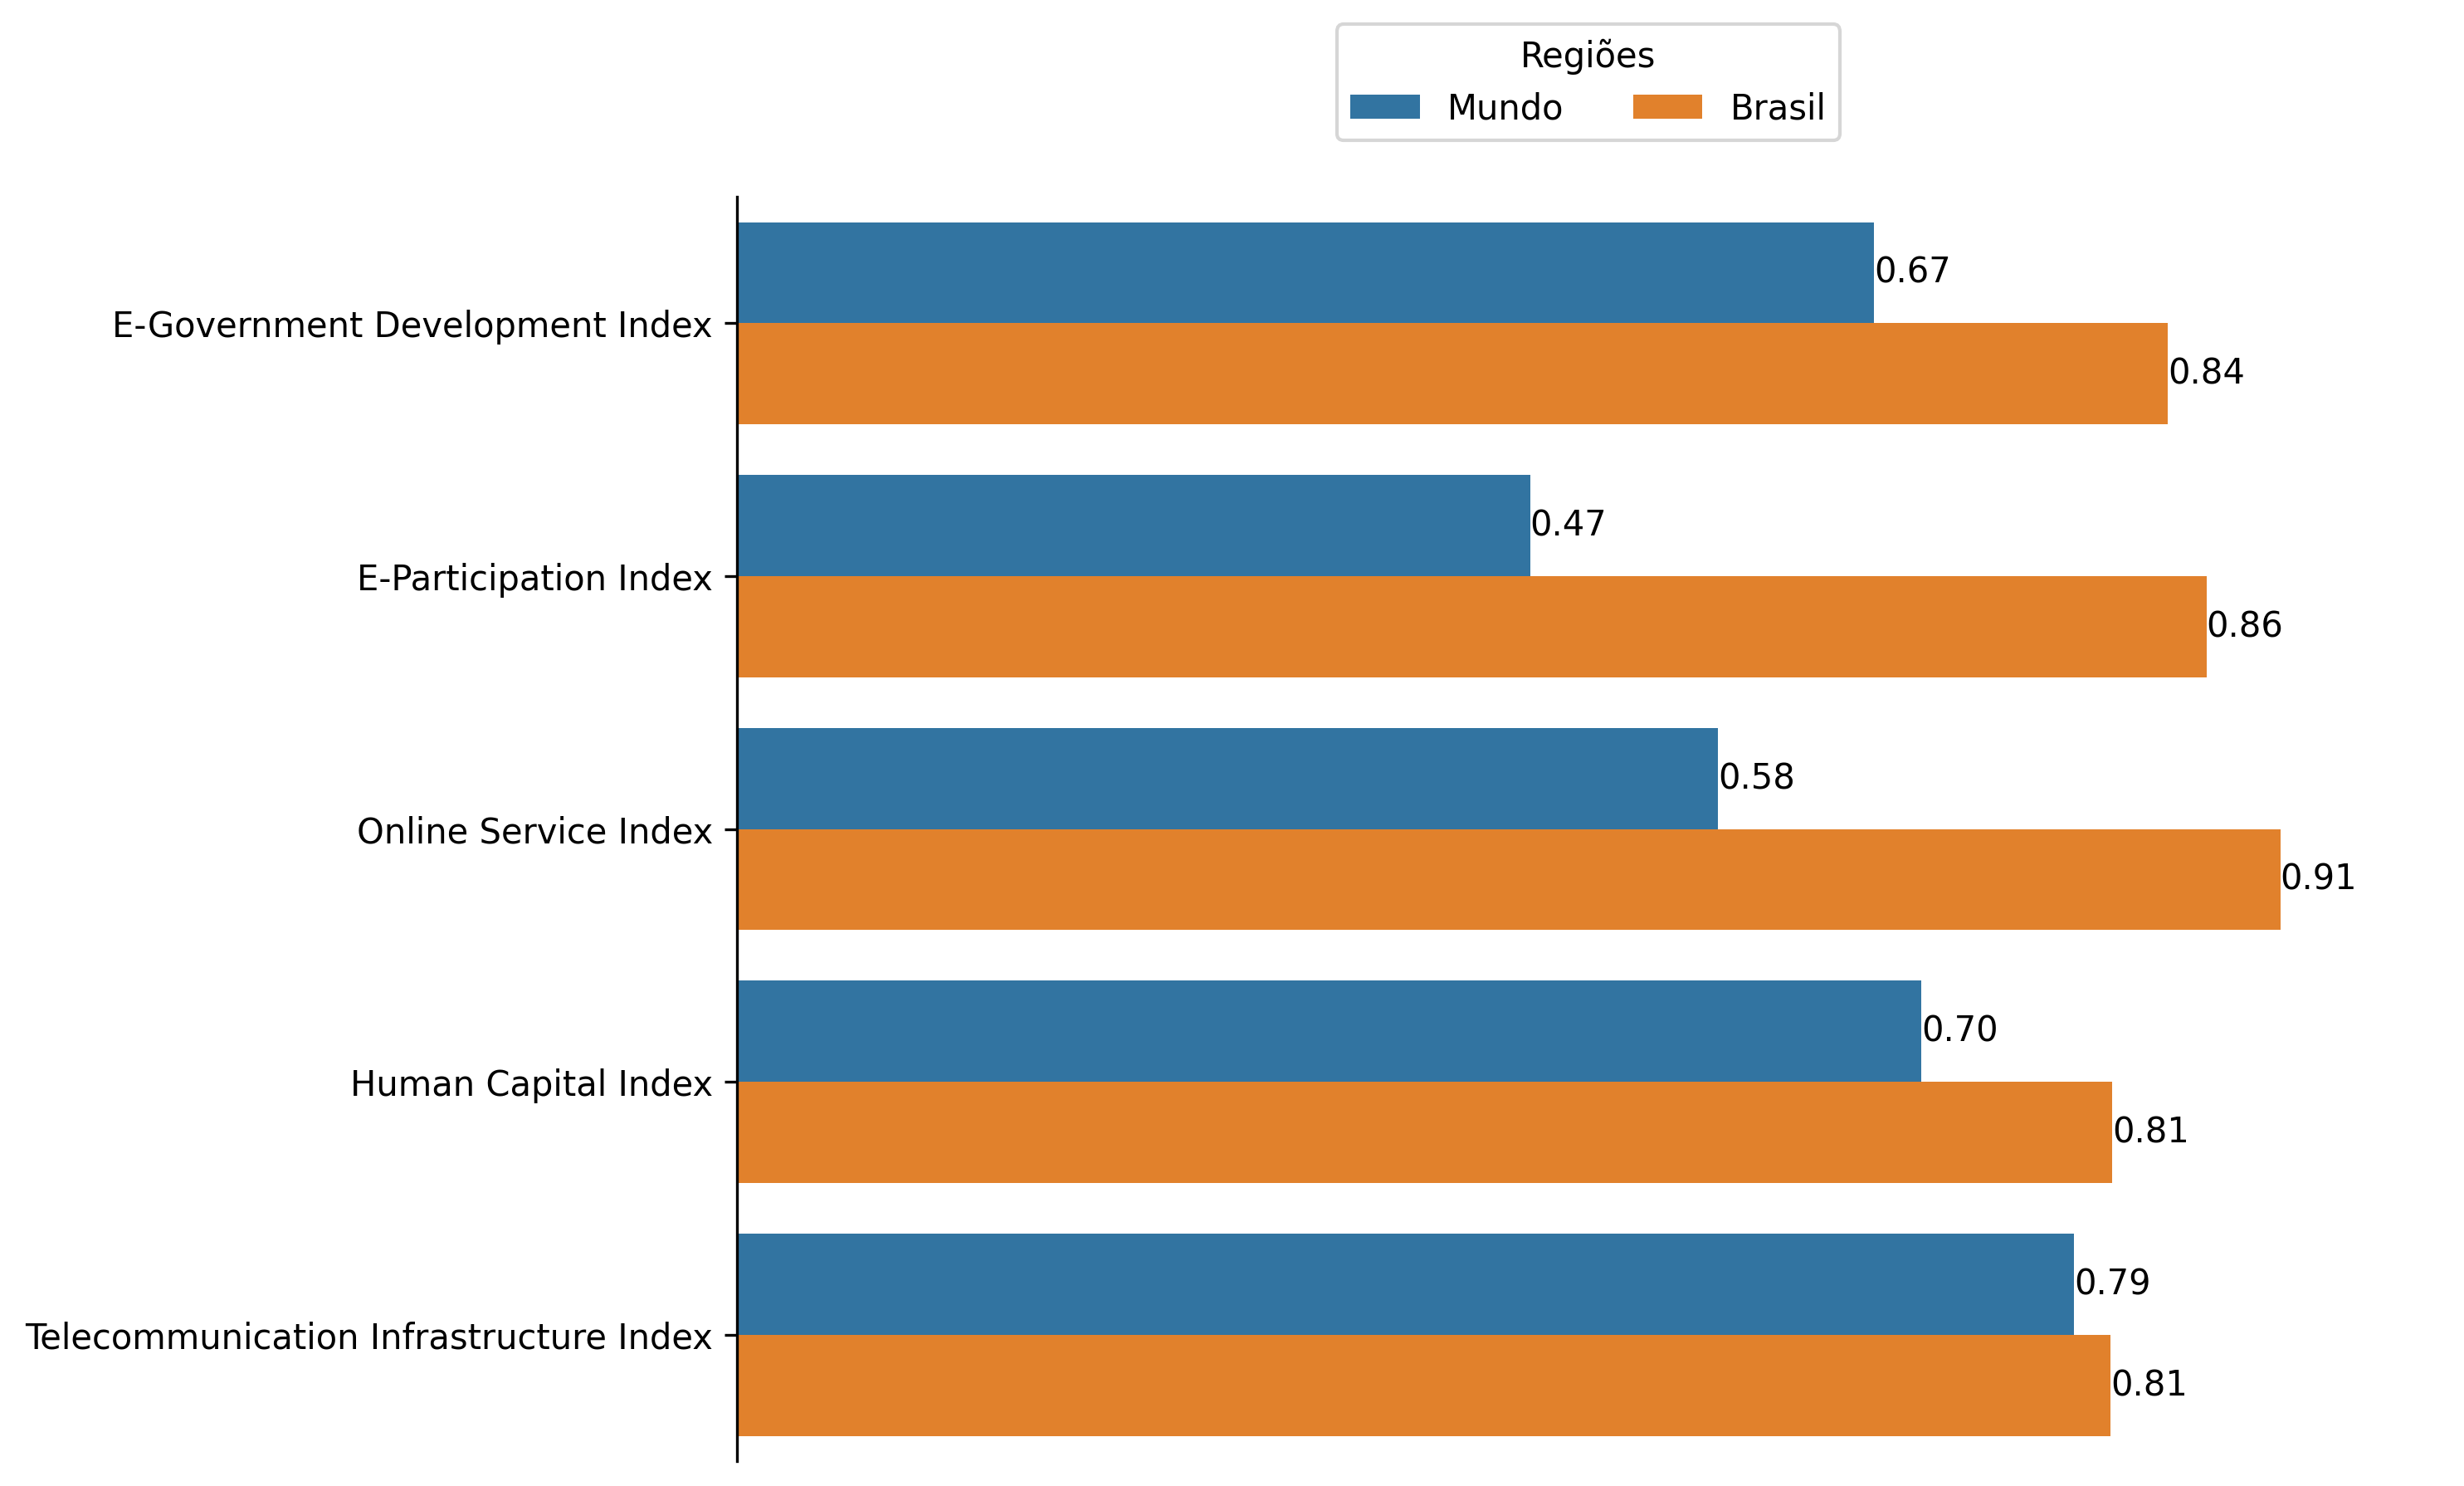
\includegraphics[width=1\linewidth]{figuras/egdi/barplot_egdi_mediamundial_brasil}
	\label{fig:barplot_egdi_mediamundial_brasil}
	\footnotesize{Fonte: baseado em \cite{ONU_EGDI_mapa}.}
\end{figure}

Nota-se como o Brasil está muito avançado em relação à média mundial.Os EGDI, \textbf{E-Participation Index}, \textbf{Online Service Index} e \textbf{Human Capital Index} foram os componentes que em mais o Brasil se detacou com 0.17, 0.29, 0.23 e 0.11 pontos acima da média mundial, respectivamente. O \textbf{Telecommunication Infrastructure Index} é o único componente em que a diferença entre à média mundial e o resultado apresentado pelo Brasil foi insiginificante (0.2 pontos de diferença).


\chapter{Worldwide Governance Indicators}
\chapter{Indicadores de TIC de governo eletrônico}
\label{indicadores_tic_egov}

A ONU tem \href{https://publicadministration.un.org/egovkb/en-us/Data/ICT-in-government}{indicadores de TIC de governo eletrônico} como algo complementar ao \hyperref[egdi]{EGDI}. Os indicadores são, conforme \cite{ONU_ICT_in_government_indicators}:

\begin{itemize}
	\item Existência de estratégia nacional de governo eletrônico ou equivalente;
	\item Existência de identidade digital para acessar ou outra forma de autenticação requirida para poder acessar serviços online;
	\item Existência de um portal de compras governamentais.
\end{itemize}

Os resultados globais dos indicadores estão presentes nas figuras \ref{fig:national_government_strategy}, \ref{fig:national_identity} e \ref{fig:procurement_portal}.

\begin{figure}[H]
	\centering
	\caption{Indicador: Existência de estratégia nacional de governo eletrônico ou equivalente}
	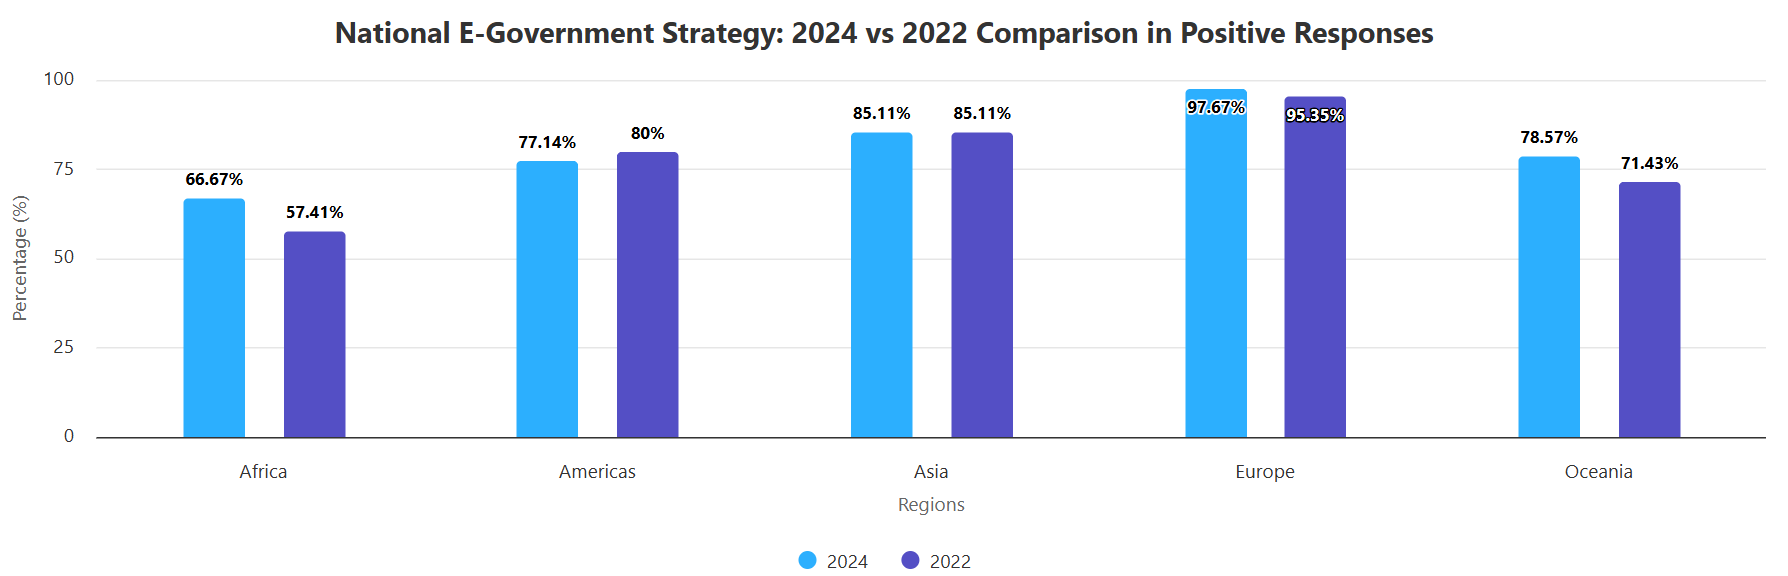
\includegraphics[width=1\linewidth]{figuras/ict_in_government/national_government_strategy}
	\label{fig:national_government_strategy}
	\footnotesize{Fonte: \cite{ONU_ICT_in_government_indicators}}
\end{figure}

\begin{figure}[H]
	\centering
	\caption{Indicador: Existência de identidade digital para acessar ou outra forma de autenticação requirida para poder acessar serviços online}
	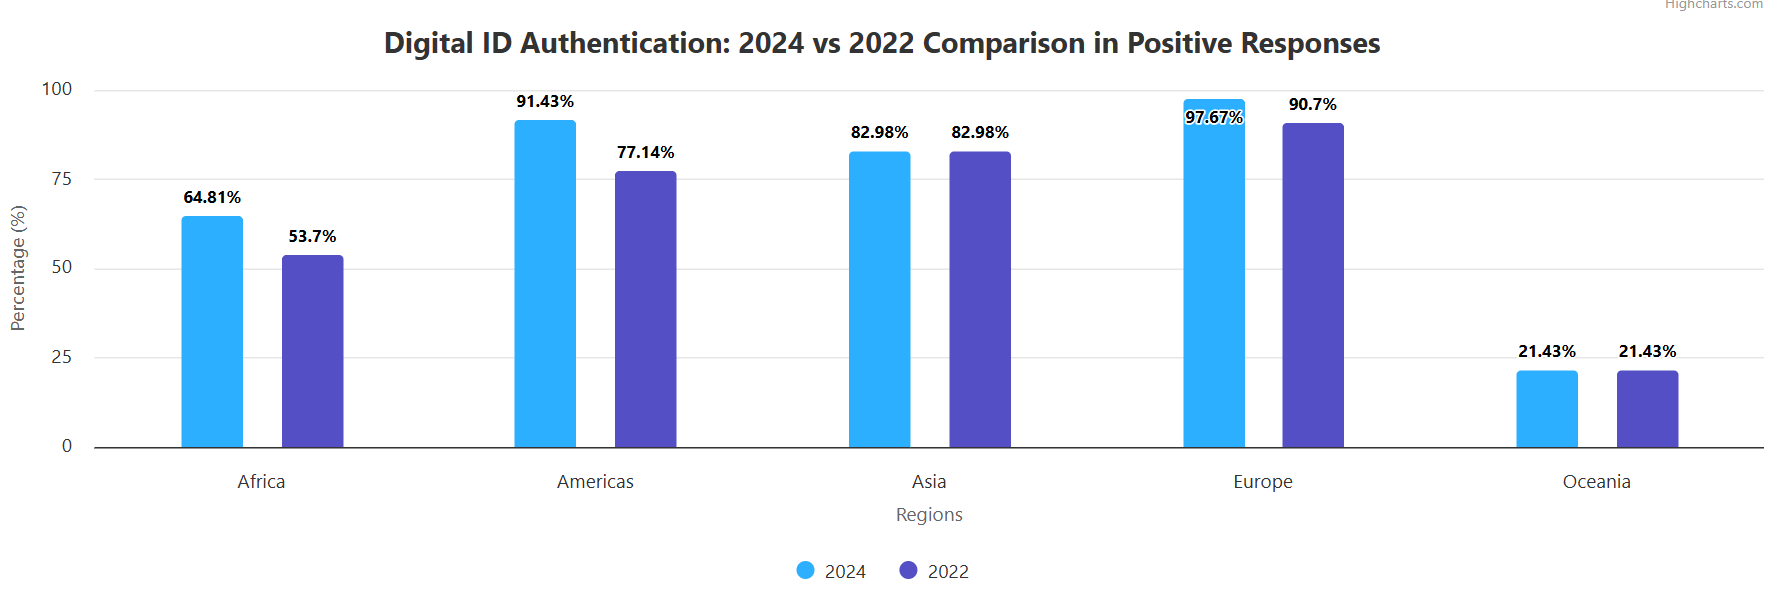
\includegraphics[width=1\linewidth]{figuras/ict_in_government/digital_identity}
	\label{fig:national_identity}
	\footnotesize{Fonte: \cite{ONU_ICT_in_government_indicators}}
\end{figure}

\begin{figure}[H]
	\centering
	\caption{Indicador: Existência de um portal de compras governamentais}
	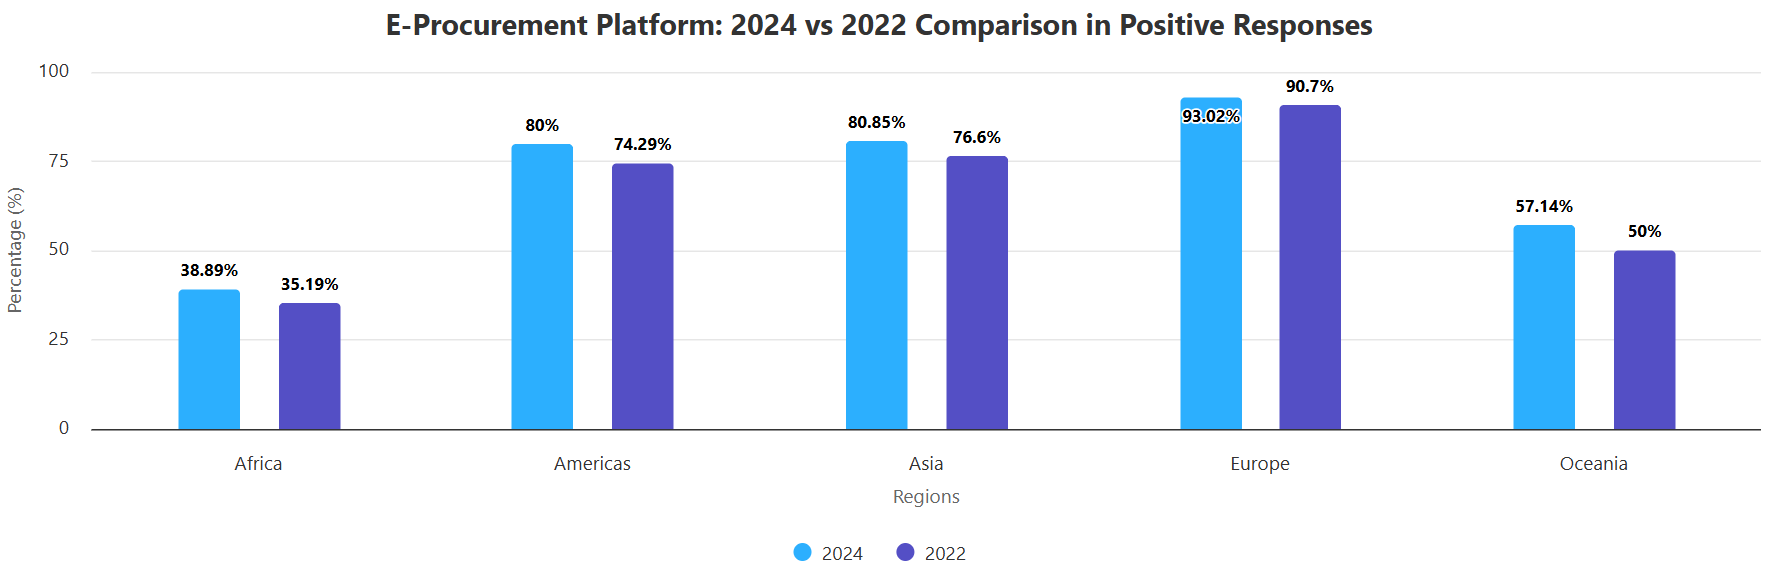
\includegraphics[width=1\linewidth]{figuras/ict_in_government/procurement_portal}
	\label{fig:procurement_portal}
	\footnotesize{Fonte: \cite{ONU_ICT_in_government_indicators}}
\end{figure}

Extraí-se das três figuras que a Europa foi o continente cujos mais respondem que têm seguem os indicadores, superando os 90\%. A Oceania foi o continente que menos implementou políticas de identidade digital para acesso a serviços online. África e Oceania tiveram um desempenho ruim na implementação de portais de compra governamentais. O continente americano apresentou bom desempenho nos três indicadores.

Como consequência da análise dos resultados presentes nas figuras \ref{fig:national_government_strategy}, \ref{fig:national_identity} e \ref{fig:procurement_portal}, buscou-se entender a seguinte situação registrada nos 2022 e 2024, anos em que os indicadores foram medidos: qual é a porcentagem de países que responderam nenhuma, uma, duas ou todas as perguntas. Elas usam sim ou não para confirmar a aplicação dos indicadores no país.

A resposta ao questionamento está presente na figura \ref{fig:indicators_answer}.

\begin{figure}[H]
	\centering
	\caption{Respostas positivas aos indicadores de TIC de governo eletrônico}
	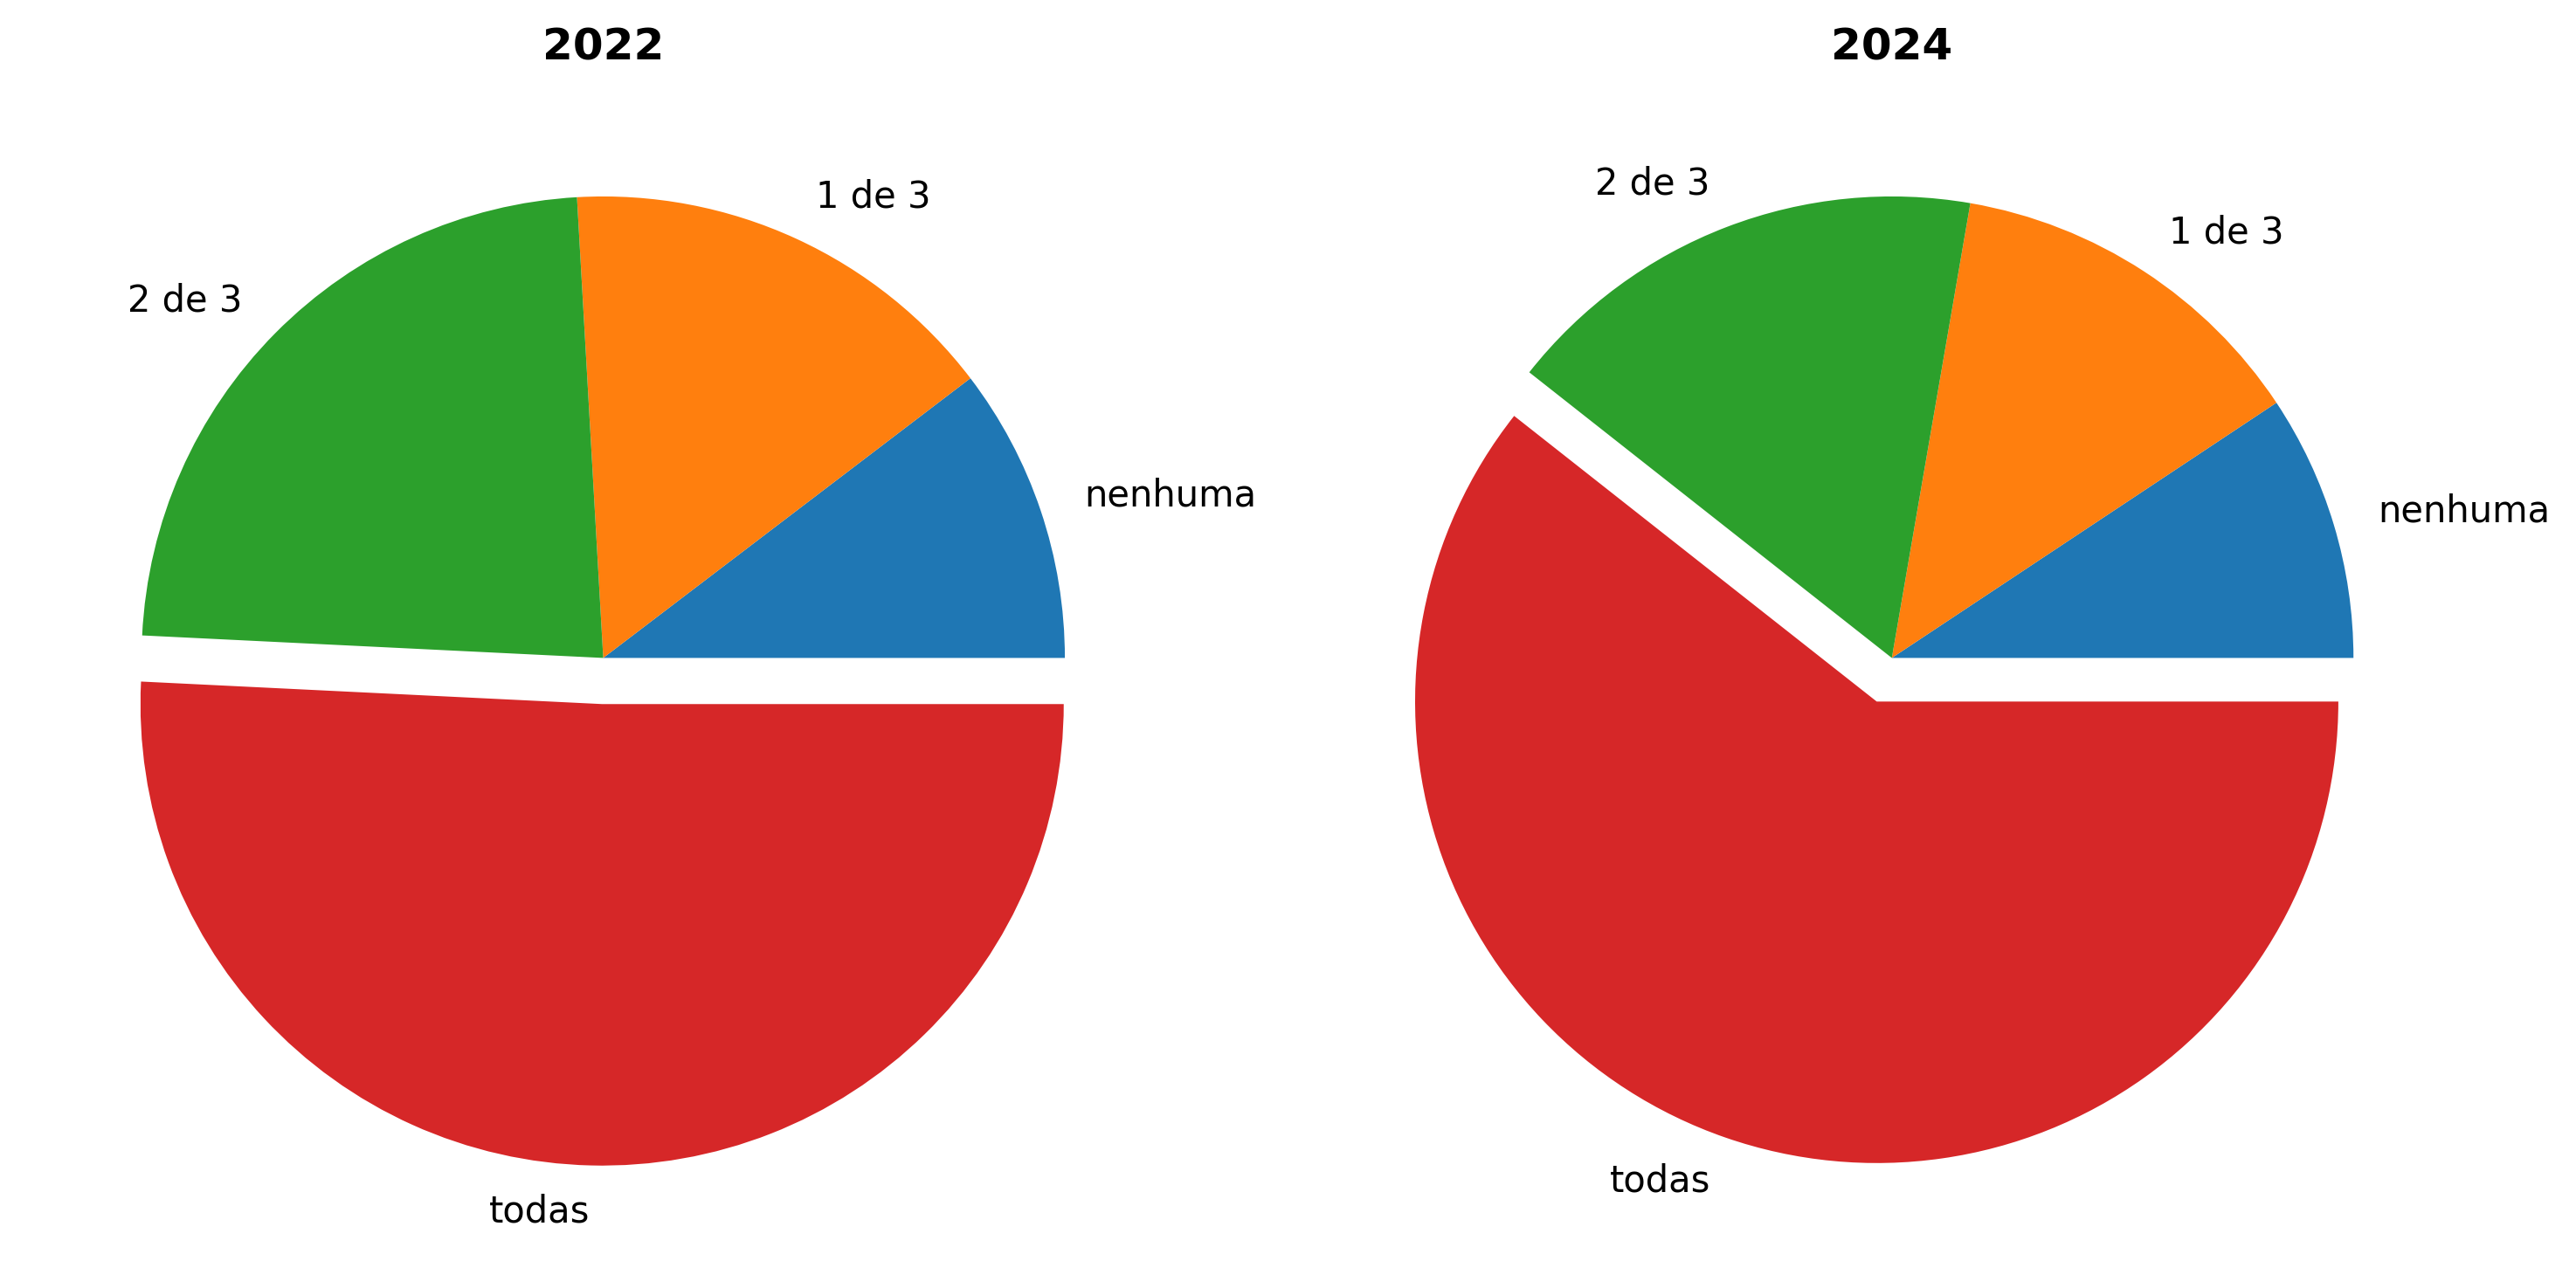
\includegraphics[width=1\linewidth]{figuras/ict_in_government/indicators_answer}
	\label{fig:indicators_answer}
	\footnotesize{Fonte: \cite{ONU_ICT_in_government_indicators}}
\end{figure}

Em 2022, metade dos países respondeu positivamente as três perguntas; em 2024, mais da metade. O Brasil faz parte desse grupo, tal como a Rússia e China. A mudança é creditada a redução do número de países que responderam positivamente 2 de 3 perguntas e passaram a responder as três positivamente. 

Além, disso a quantidade de países que responderam positivamente 1 de 3 perguntas e nenhuma se igualou em 2024, sendo os países que responderam 1 de 3 perguntas era maior do que os que responderam nenhuma.

\subsubsection{Coeficiente de correlação: indicadores de TIC de governo eletrônico  comparados com o PIB \textit{per capita} PPC e os gastos públicos (\% do PIB)}.

Com base na seção \ref{indicadores_tic_egov}, buscou-se entender se há correlação entre os indicadores de TIC de governo eletrônico e os PIB \textit{per capita} PPC e os gastos públicos (\% do PIB).

\begin{figure}[H]
	\centering
	\caption{Diagrama de Dispersão: indicadores de TIC de governo eletrônico e PIB \textit{per capita} PPC}
	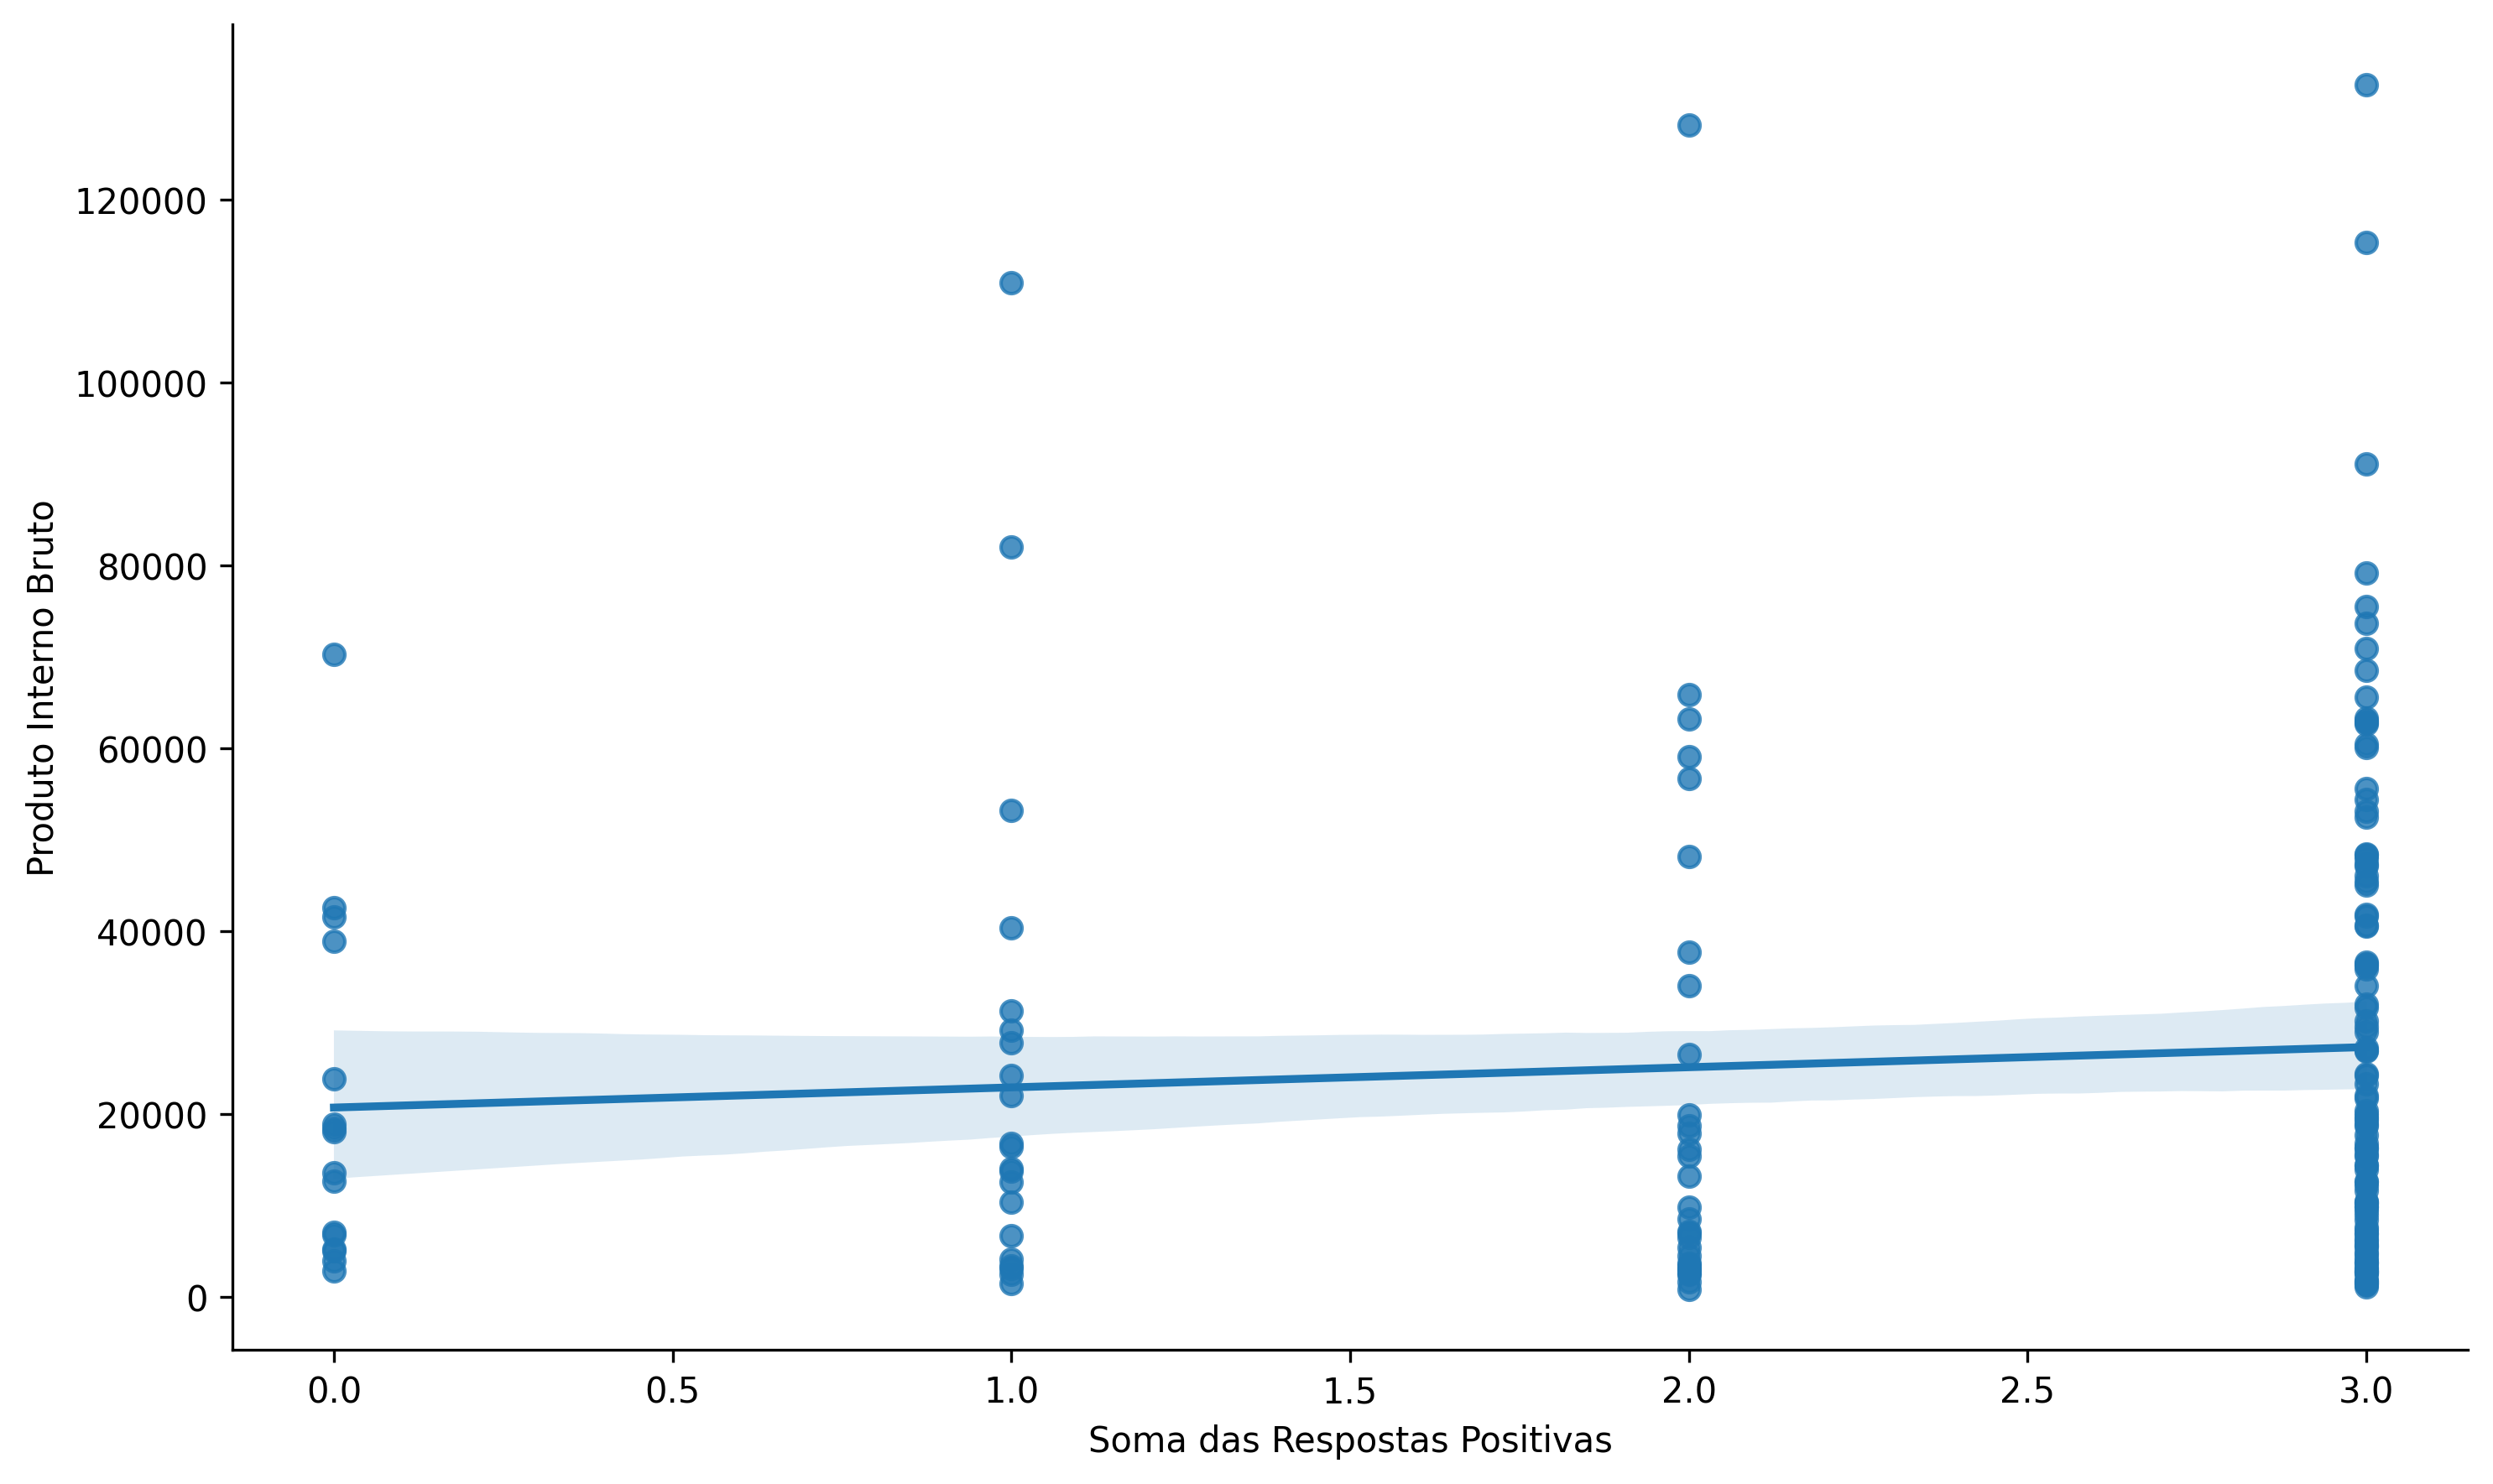
\includegraphics[width=1\linewidth]{figuras/ict_in_government/dispersao_ticegov_pib}
	\label{fig:dispersao_ticegov_pib}
	\footnotesize{Fonte: baseado em \cite{WB_pib_per_capita_países} e \cite{ONU_ICT_in_government_indicators}}
\end{figure}

Como o diagrama de dispersão presente na figura \ref{fig:dispersao_ticegov_pib} e apresenta grande dispersão em relação à tendência, optou-se pelo uso do coeficiente de correlação de Spearman. A alta dispersão em relação à tendência é um indicativo de um coeficiente de correlação neutro ou baixo. O coeficiente de correlação (0.1) indicam que os indicadores de TIC de governo eletrônico não são afetados pelo PIB \textit{per capita} PPC, e vice-versa.

Outra análise feita foi a comparação entre os indicadores de TIC de governo eletrônico e os gastos governamentais.

\begin{figure}[H]
	\centering
	\caption{Diagrama de Dispersão: indicadores de TIC de governo eletrônico e gastos governamentais (\% do PIB)}
	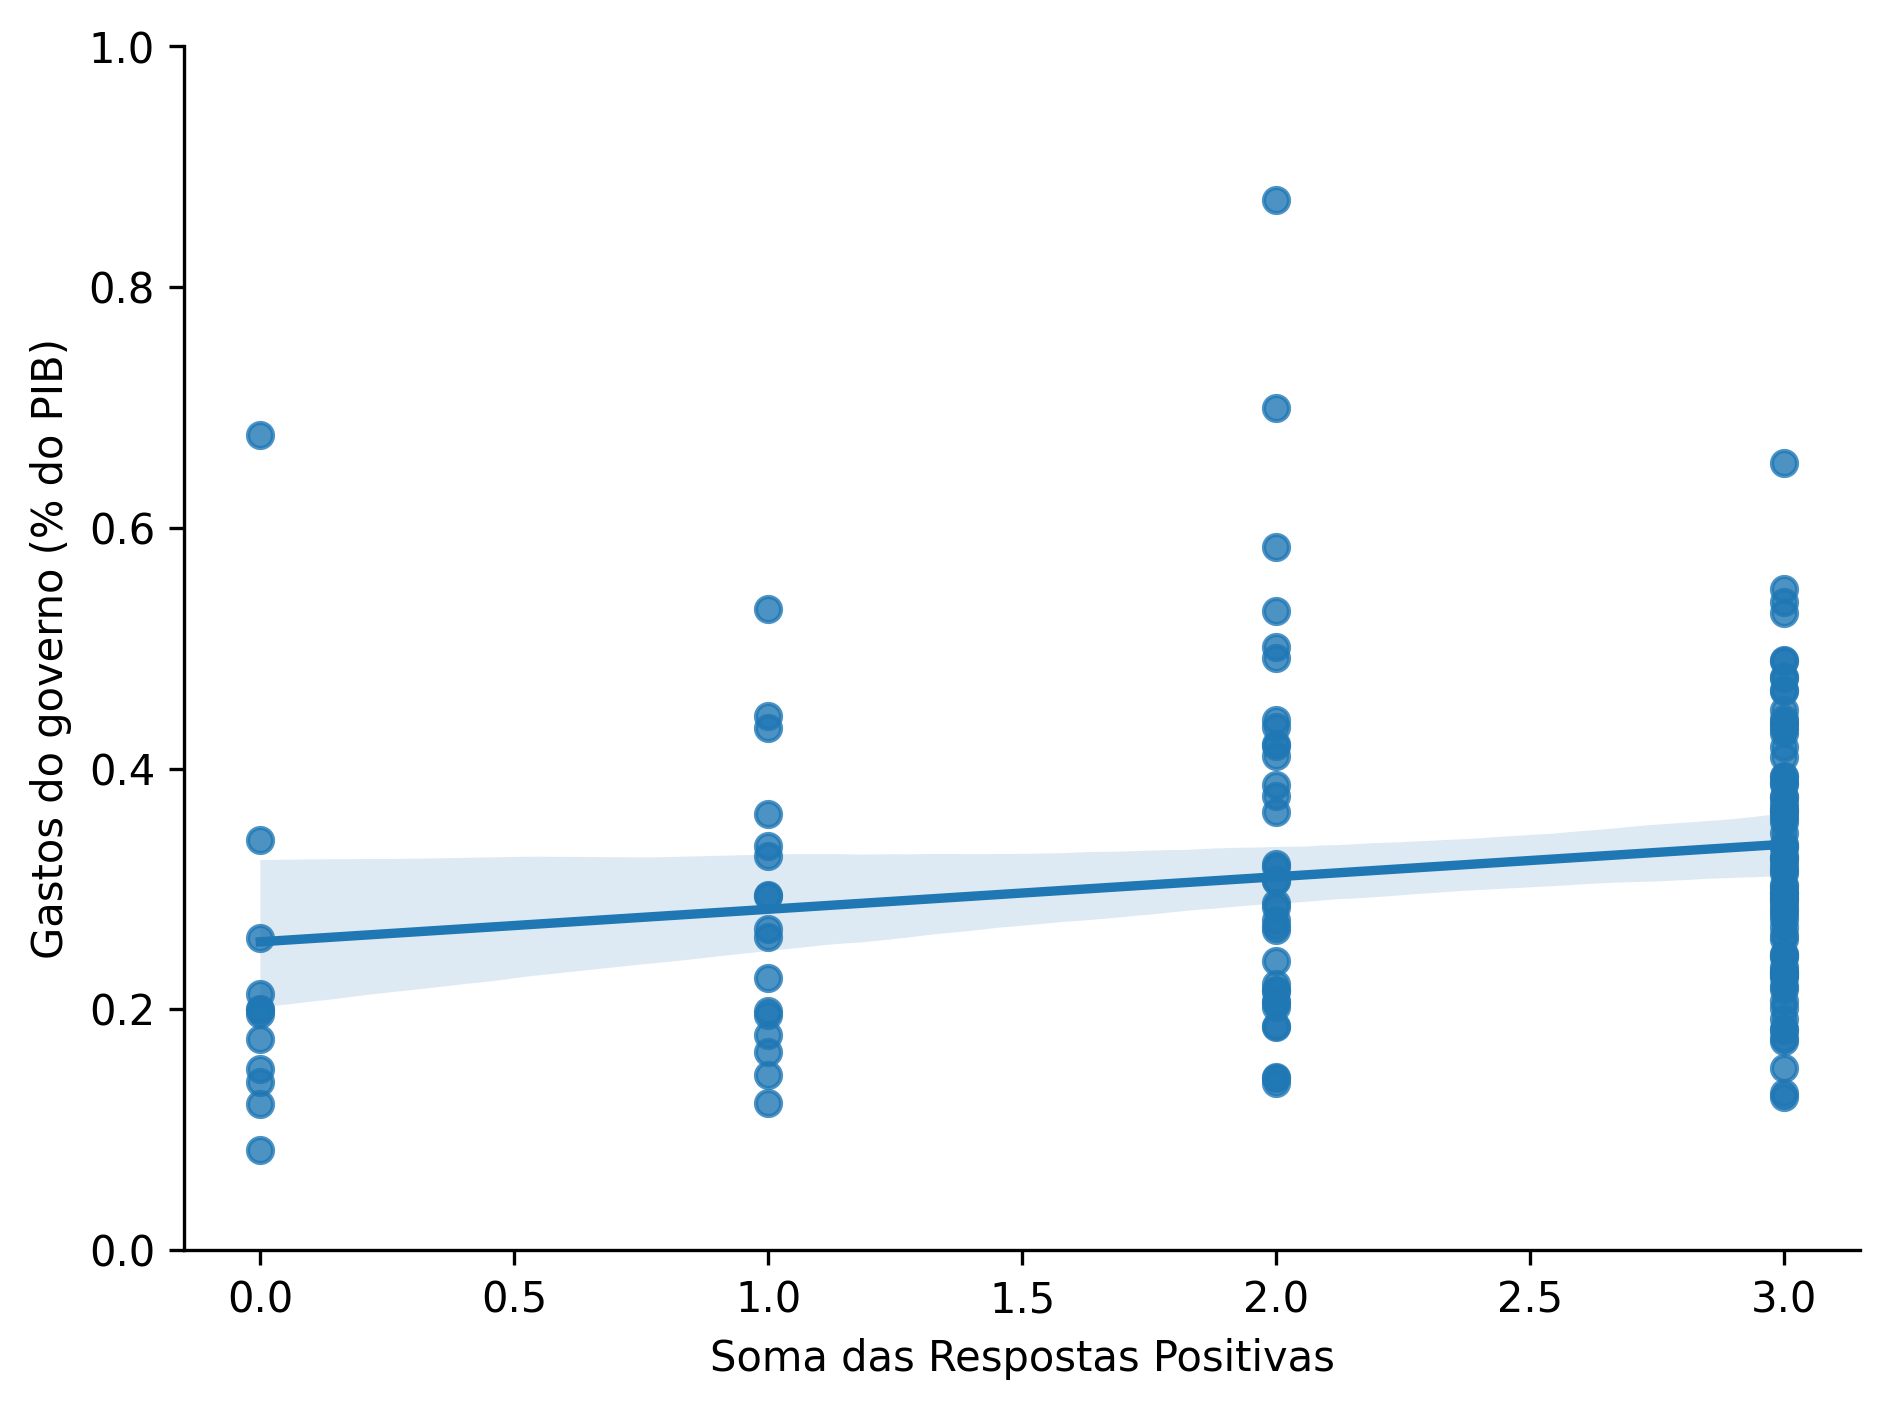
\includegraphics[width=1\linewidth]{figuras/egdi/dispersao_ticegov_govexpenditure}
	\label{fig:dispersao_ticegov_govexpenditure}
	\footnotesize{Fonte: baseado em \cite{FMI_gov_expenditure} e \cite{ONU_ICT_in_government_indicators}}
\end{figure}

Para compreender melhor o diagrama de dispersão, foi usado o coeficiente de correlação de Spearman. A sua escolha foi motivada pela grande presença de pontos extremos. O coeficiente de correlação encontrada foi 0.23. O referido coeficiente indica uma correlação positiva muito fraca entre os gastos do governo e a soma das respostas positivas. 
\chapter{Digitalização do Poder Público Brasileiro}

"Este capítulo mergulha no processo de digitalização do setor público brasileiro, analisando a evolução das políticas e o impacto da tecnologia na relação entre o Estado e o cidadão. Inicialmente, exploramos o conceito de governo eletrônico, compreendido como a base tecnológica que otimiza a gestão e a oferta de serviços. Em seguida, foi detalhado seus benefícios e, de forma crítica, foi examinado as limitações que levaram à necessidade de uma abordagem mais abrangente: o governo digital.

\section{Contextualização do governo eletrônico}

\cite{tavares2022governo} afirma que as políticas públicas são a forma como se resolve os problemas da sociedade e o controle social é a forma como o cidadão interage, fiscaliza e questiona as soluções definidas para esses problemas. 

\cite{rover2009introduccao} argumenta que a interação entre as novas tecnologias, a sociedade e o Poder Público emoldura um momento único do qual emergem, simultaneamente, desafios enormes e vantagens sociais incríveis. Neste contexto, o aparecimento do governo eletrônico é uma decorrência das velhas e novas demandas da sociedade.

Para \cite{rover2009introduccao}, governo eletrônico é uma infra-estrutura única de comunicação compartilhada por diferentes órgãos públicos a partir da qual a TIC é usada de forma intensiva para melhorar a gestão pública e o atendimento ao cidadão.

Adicionalmente, como é entendido por \cite{rover2009introduccao}, o objetivo do governo eletrônico é colocar o governo ao alcance de todos, ampliando a transparências das suas ações e incrementando a participação cidadã, almejando a universalização de serviços.

\cite{singh2007country} projeta que a maturidade do governo eletrôncio pode ser considerada razoavelmente dependente de como está o estado da infraestrutura de TIC, em razão da sua capacidade de limitar o acesso aos serviços públicos digitais. 

Para \cite{singh2007country}, países com PIB per capita altos estão em melhor posição de dispor de infraestruturas difundidas, alta qualidade e físicas de TIC. Com altos níveis de acesso às TIC, os cidadãos tem uma tendência maior de usar serviços públicos digitais.

Quando os cidadãos passam a adotar os serviços públicos digitais, segundo \cite{singh2007country}, facilita ao poder público a transação completa dos serviços públicos presenciais para os digitais. A referida mudança pode ajudar na economia de recursos públicos, definindo um círculo virtuoso que justifica os investimentos em governo eletrônico.

\section{Benefícios do governo eletrônico}

Diversos autores destacam o impacto positivo do governo eletrônico na sociedade.  \cite{martins2018war} cita que os resultados encontrados indicam claramente que níveis mais altos de governo eletrônico estão associados a melhores resultados no combate à corrupção. Para \cite{kotenok2020government}, o impacto do governo eletrônico pode impulsionar a inovação ou até mesmo ser um componente importante para entender como a economia é transformada   devido à tecnologia.

\cite{martins2022digital} um nível alto de governo eletrônico podem facilitar negócios pela   diminuição do fardo das regulações em diversas áreas de negócio. \cite{sugiarti2024effect} sua pesquisa examinou a relação entre governo eletrônico e corrupção nos   estados dos Estados Unidos encontraram que o governo eletrônico aumentou   tanto as condenações por corrupção, quanto a percepção de corrupção.

Para \cite{ziolo2022government}, na União Europeia (até 2020) observou-se a correlação observada entre o nível de desenvolvimento do governo eletrônico e as áreas ambiental, social e econômica parece ser de grande importância, pois implica que a digitalização dos processos administrativos pode ter um impacto real no desenvolvimento   sustentável, promovendo, assim, mudanças positivas em todas as suas três esferas.

\section{Foco do governo eletrônico}

Contudo, para \cite{de2020governo} o foco das políticas de governo eletrônico, em geral, permanece o mesmo: aprimorar processos internos de  trabalho, sem alterações significativas na cultura e na lógica burocráticas sobre as quais se estruturam as relações que se estabelecem entre a administração pública e os cidadãos.

Assim, para \cite{cristovam2020governo} a Administração Pública brasileira tem usado as TIC no incremento de suas rotinas burocráticas. Há, ainda, o crescente uso dessas tecnologias na promoção do acesso à informação aos cidadãos. Mas ambos são usos na esteira do dito Governo eletrônico.

Consequentemente, conforme \cite{cristovam2020governo}, para se distanciar do governo eletrônico e poder implementar o governo digital, pois não se deve almeja somente o emprego incremental de TICs e a viabilização do acesso à informação, mas vai além, corporificando direitos sociais por intermédio do espaço digital.

Nesse sentido, quando \cite{cristovam2020governo} afirma que as TIC podem contribuir para a inovação e o fomento da prestação de serviços públicos adequados e atuais para todos os cidadãos, comportando as dimensões democrática e social impostas pela ordem jurídica constitucional vigente, há convergência com a ideia expressa por \cite{kotenok2020government} com os autores anteriores.

No dado contexto, \cite{alenezi2022understanding} afirma que sua pesquisa destaca que um ambiente efetivo e favorável, força de trabalho qualificada, liderança, políticas públicas e regulações são os fatores-chave do sucesso que podem encorajar e facilitar a rápida adaptação da transformação digital nas organizações do setor público.

\section{Entendendo o governo eletrônico no Brasil}
	
Como forma de entender o uso do governo eletrônico no Brasil, optou-se por \cite{tic_domicilios_2024}, devido ao seu objetivo de mapear o acesso às TIC nos domicílios urbanos e rurais do país e as suas formas de uso por indivíduos de 10 anos de idade ou mais. E ao fato de que o uso de governo eletrônico ser uma das suas áreas de investigação.

Em razão da continuidade das pesquisa TIC Domicílios desde 2005, escolheu-se o último de pesquisa (\textbf{2024}) da Cetic.BR. O tópico G foi o escolhido. Dele serão usados todos os seus indicadores G1, G2, G2A, G3. O primeiro, o G1, revelou o percentual de uso de governo eletrônico por indivíduos, cujo resultado está presente na figura \ref{fig:mapa_coropletico_tic_domicilio_g1}.

\begin{figure}[H]
	\centering
	\caption{Indicador G1: Uso de governo eletrônico por região do Brasil (em \%)}
	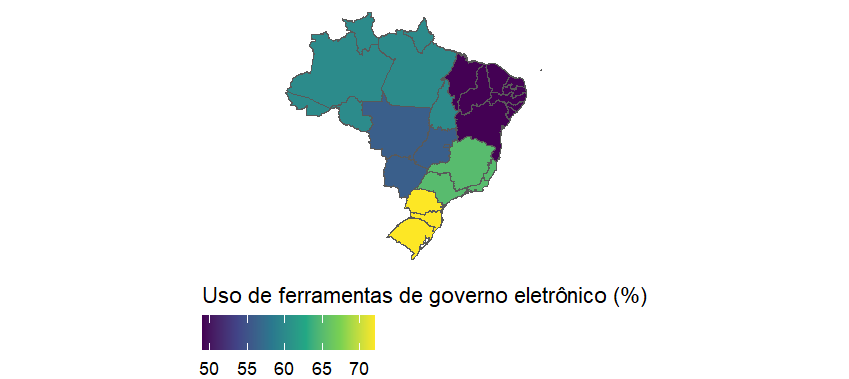
\includegraphics[width=1\linewidth]{figuras/mapa_coropletico_tic_domicilios_2024_g1}
	\label{fig:mapa_coropletico_tic_domicilio_g1}
	\footnotesize{Fonte: \cite{tic_domicilios_2024_g1}.}
\end{figure}

A figura \ref{fig:mapa_coropletico_tic_domicilio_g1} representa os resultados do indicador G1. As regiões Sul e Sudeste são as regiões que mais usam o governo eletrônico, seguidas das regiões Centro-Oeste e Norte. Por último, está o Nordeste.

O indicador G2 complementa o G1 ao especificar quais grupos de funções de governo eletrônico foram os mais usados. O indicador G2 tem os seguintes critérios:

\begin{itemize}
	\item Documentos pessoais, como RG, CPF, passaporte ou carteira de trabalho (G2-1)
	Saúde pública, como agendamento de consultas, remédios ou outros serviços do sistema público de saúde (G2-2).
	\item Educação pública, como Enem, Prouni, matrículas em escolas ou universidades públicas (G2-3).
	\item Direito do trabalhador ou previdência social, como INSS, FGTS, seguro-desemprego, auxílio-doença ou aposentadoria (G2-4).
	\item Impostos e taxas governamentais, como declaração de imposto de renda, IPVA ou IPTU (G2-5).
	\item Polícia e segurança, como boletim de ocorrência, antecedentes criminais ou denúncias (G2-6).
	\item Transporte público ou outros serviços urbanos, como limpeza e conservação de vias, iluminação (G2-7).
\end{itemize}

As figuras seguintes detalham como cada critério é usado por região.

\begin{figure}[H]
	\centering
	\caption{Indicador G2: critérios 1 e 2 (em \%)}
	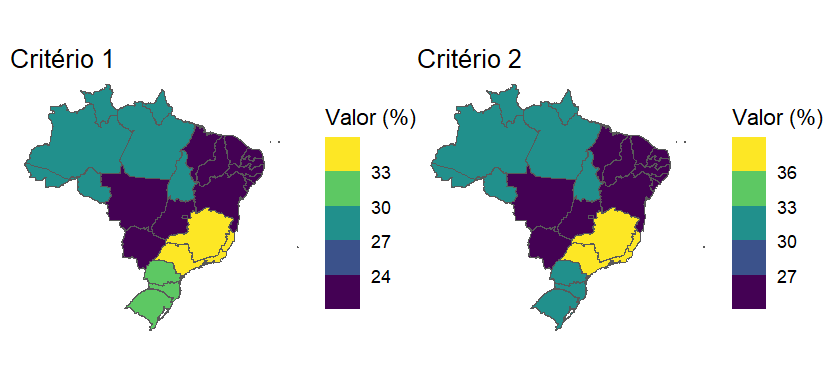
\includegraphics[width=1\linewidth]{figuras/mapa_coropletico_tic_domicilios_2024_g2_1_2.png}
	\label{fig:mapa_coropletico_tic_domicilios_2024_g2_1_2}
	\footnotesize{Fonte: \cite{tic_domicilios_2024_g2}.}
\end{figure}

Quando se trata do indicador G2-1, as regiões que mais buscaram serviços públicos relativos a documentos pessoais, como RG, CPF, passaporte ou carteira de trabalho foram as Norte, Sudeste e Sul;

Quando se trata do indicador G2-2, apenas o Nordeste foi a região que menos uso serviços públicos relativos à saúde pública, como agendamento de consultas, remédios ou outros serviços do sistema público de saúde.

\begin{figure}[H]
	\centering
	\caption{Indicador G2: critérios 3 e 4 (em \%)}
	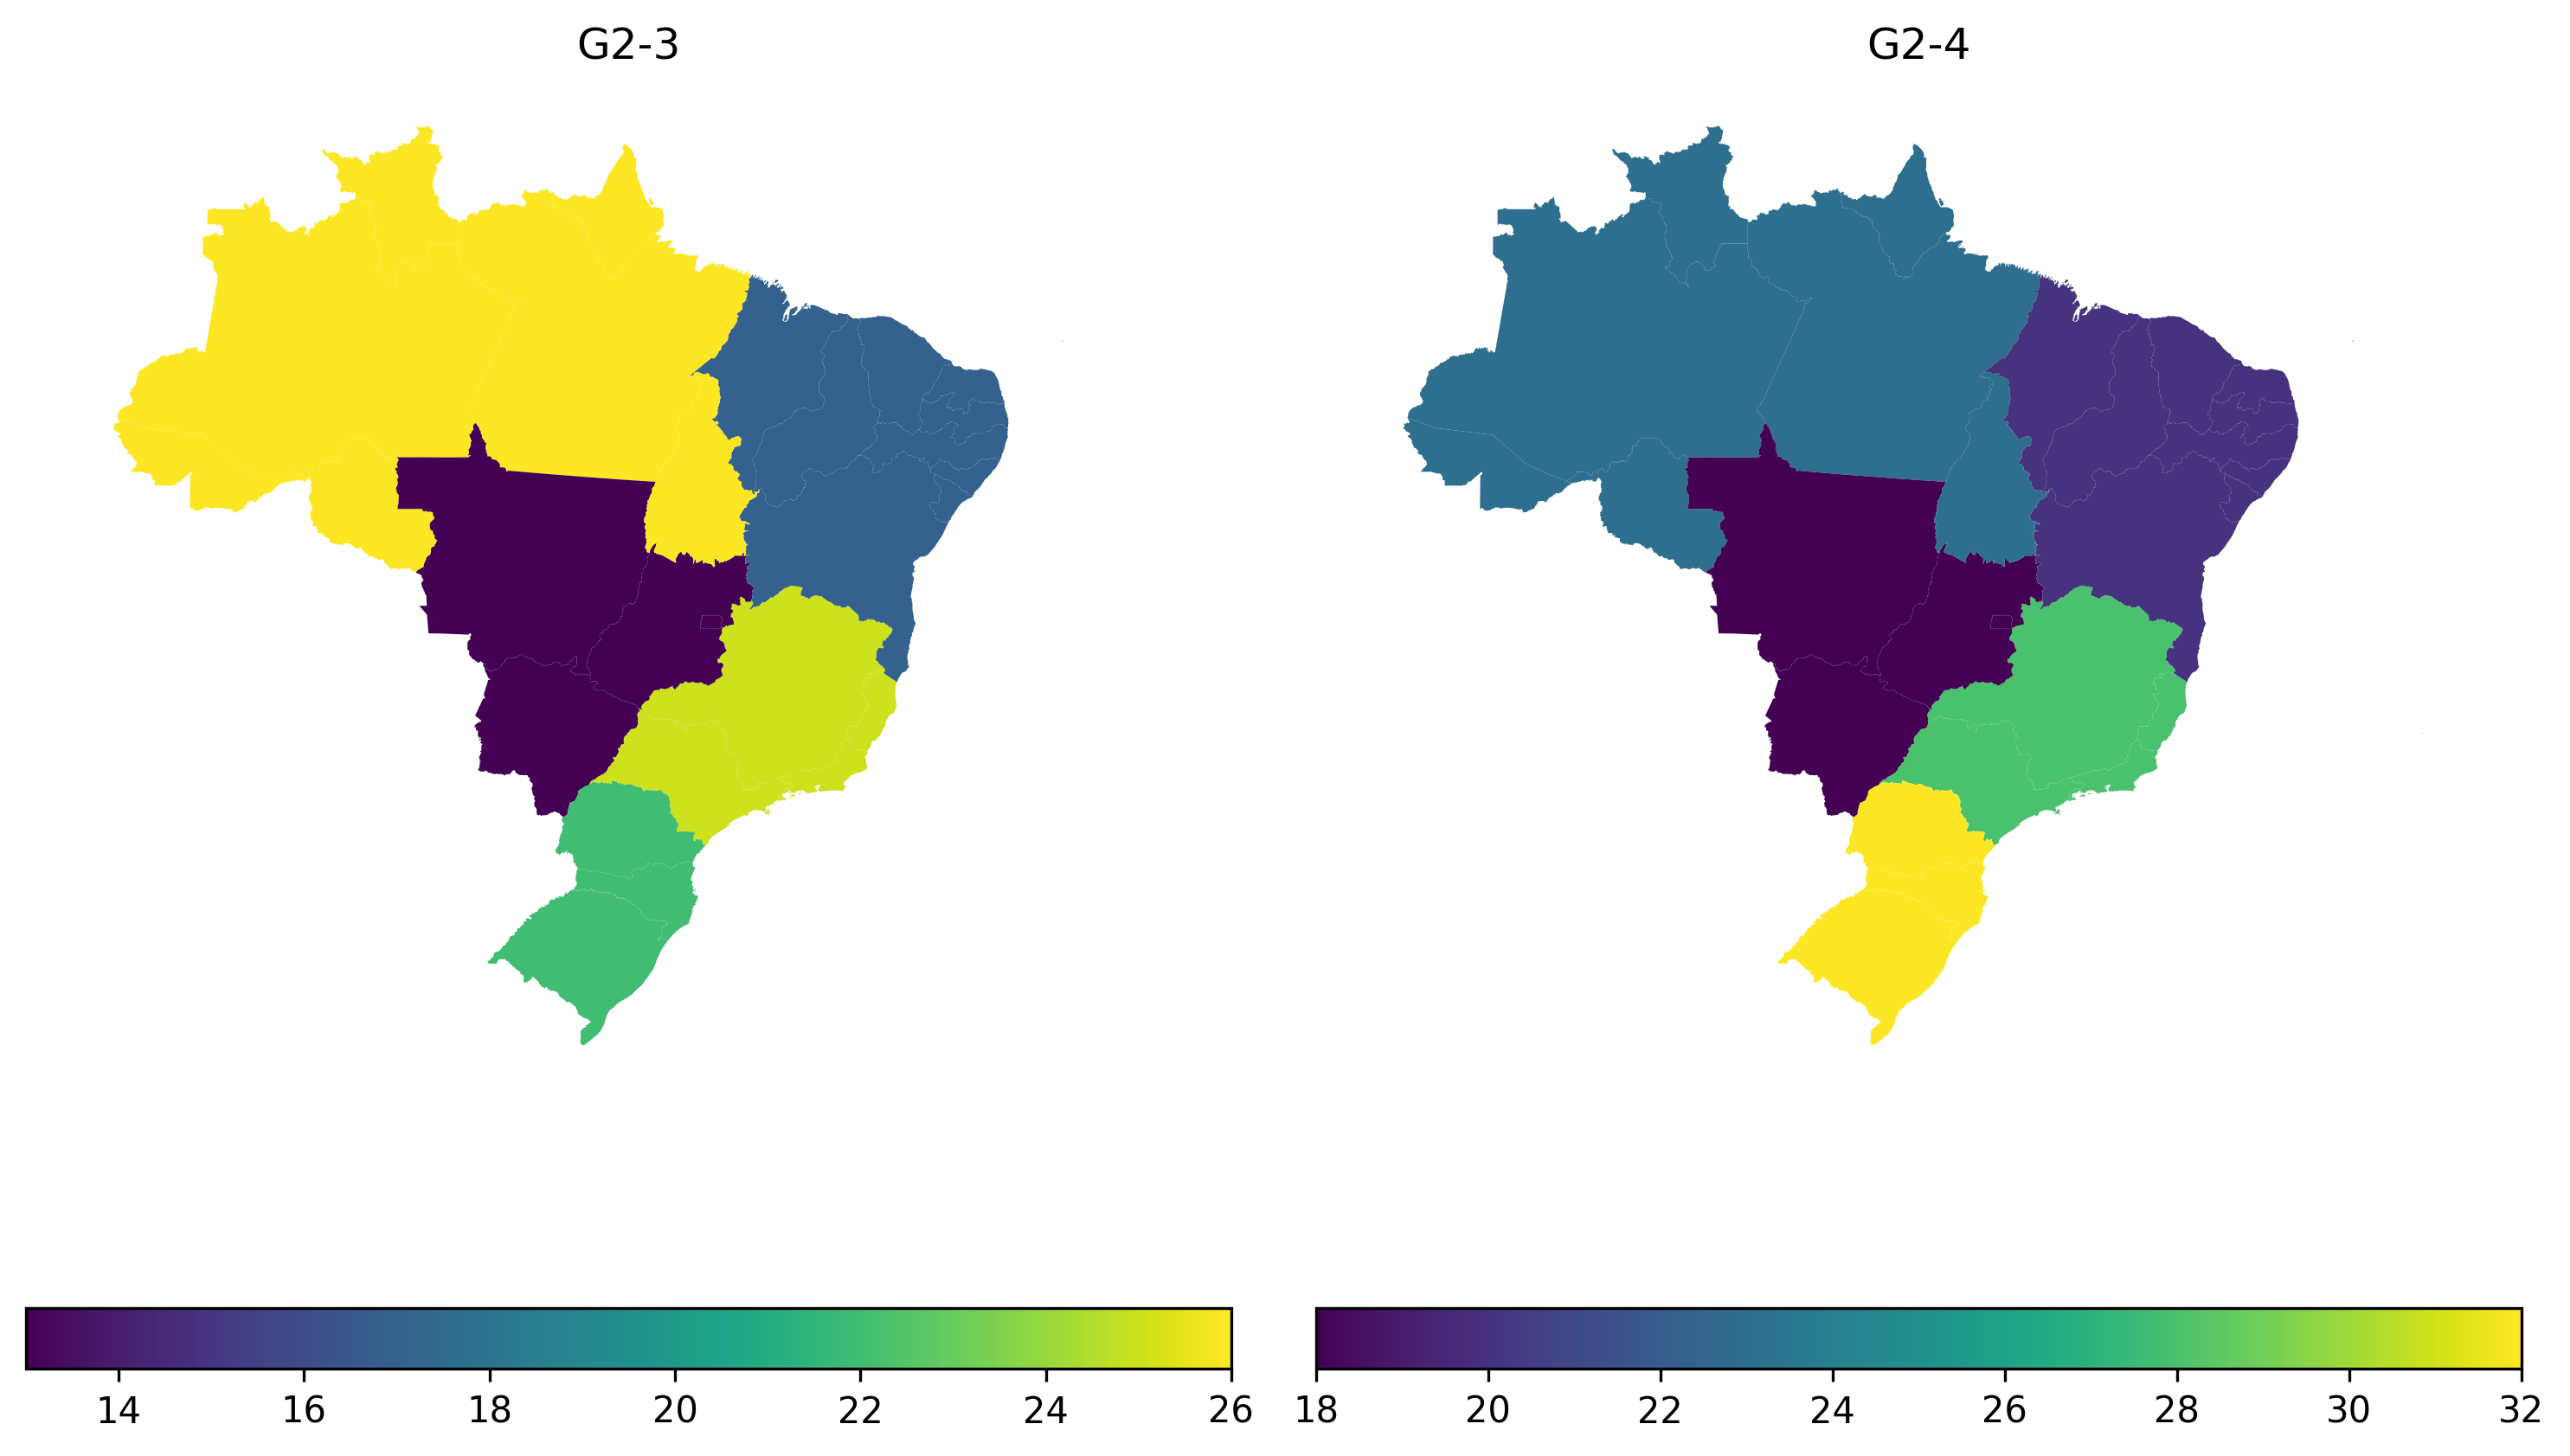
\includegraphics[width=1\linewidth]{figuras/mapa_coropletico_tic_domicilios_2024_g2_3_4.png}
	\label{fig:mapa_coropletico_tic_domicilios_2024_g2_3_4}
	\footnotesize{Fonte: \cite{tic_domicilios_2024_g2}.}
\end{figure}

Quando se trata do indicador G2-3, as regiões que mais usam serviços públicos relativos à educação pública, como Enem, Prouni, matrículas em escolas ou universidades públicas foram a Norte e a Sudeste.

Quando se trata do indicador G2-4, as regiões que mais usar serviços públicos relativos ao direito do trabalhador ou previdência social, como INSS, FGTS, seguro-desemprego, auxílio-doença ou aposentadoria foram as Sudeste e a Sul.

\begin{figure}[H]
	\centering
	\caption{Indicador G2: critérios 5 e 6 (em \%)}
	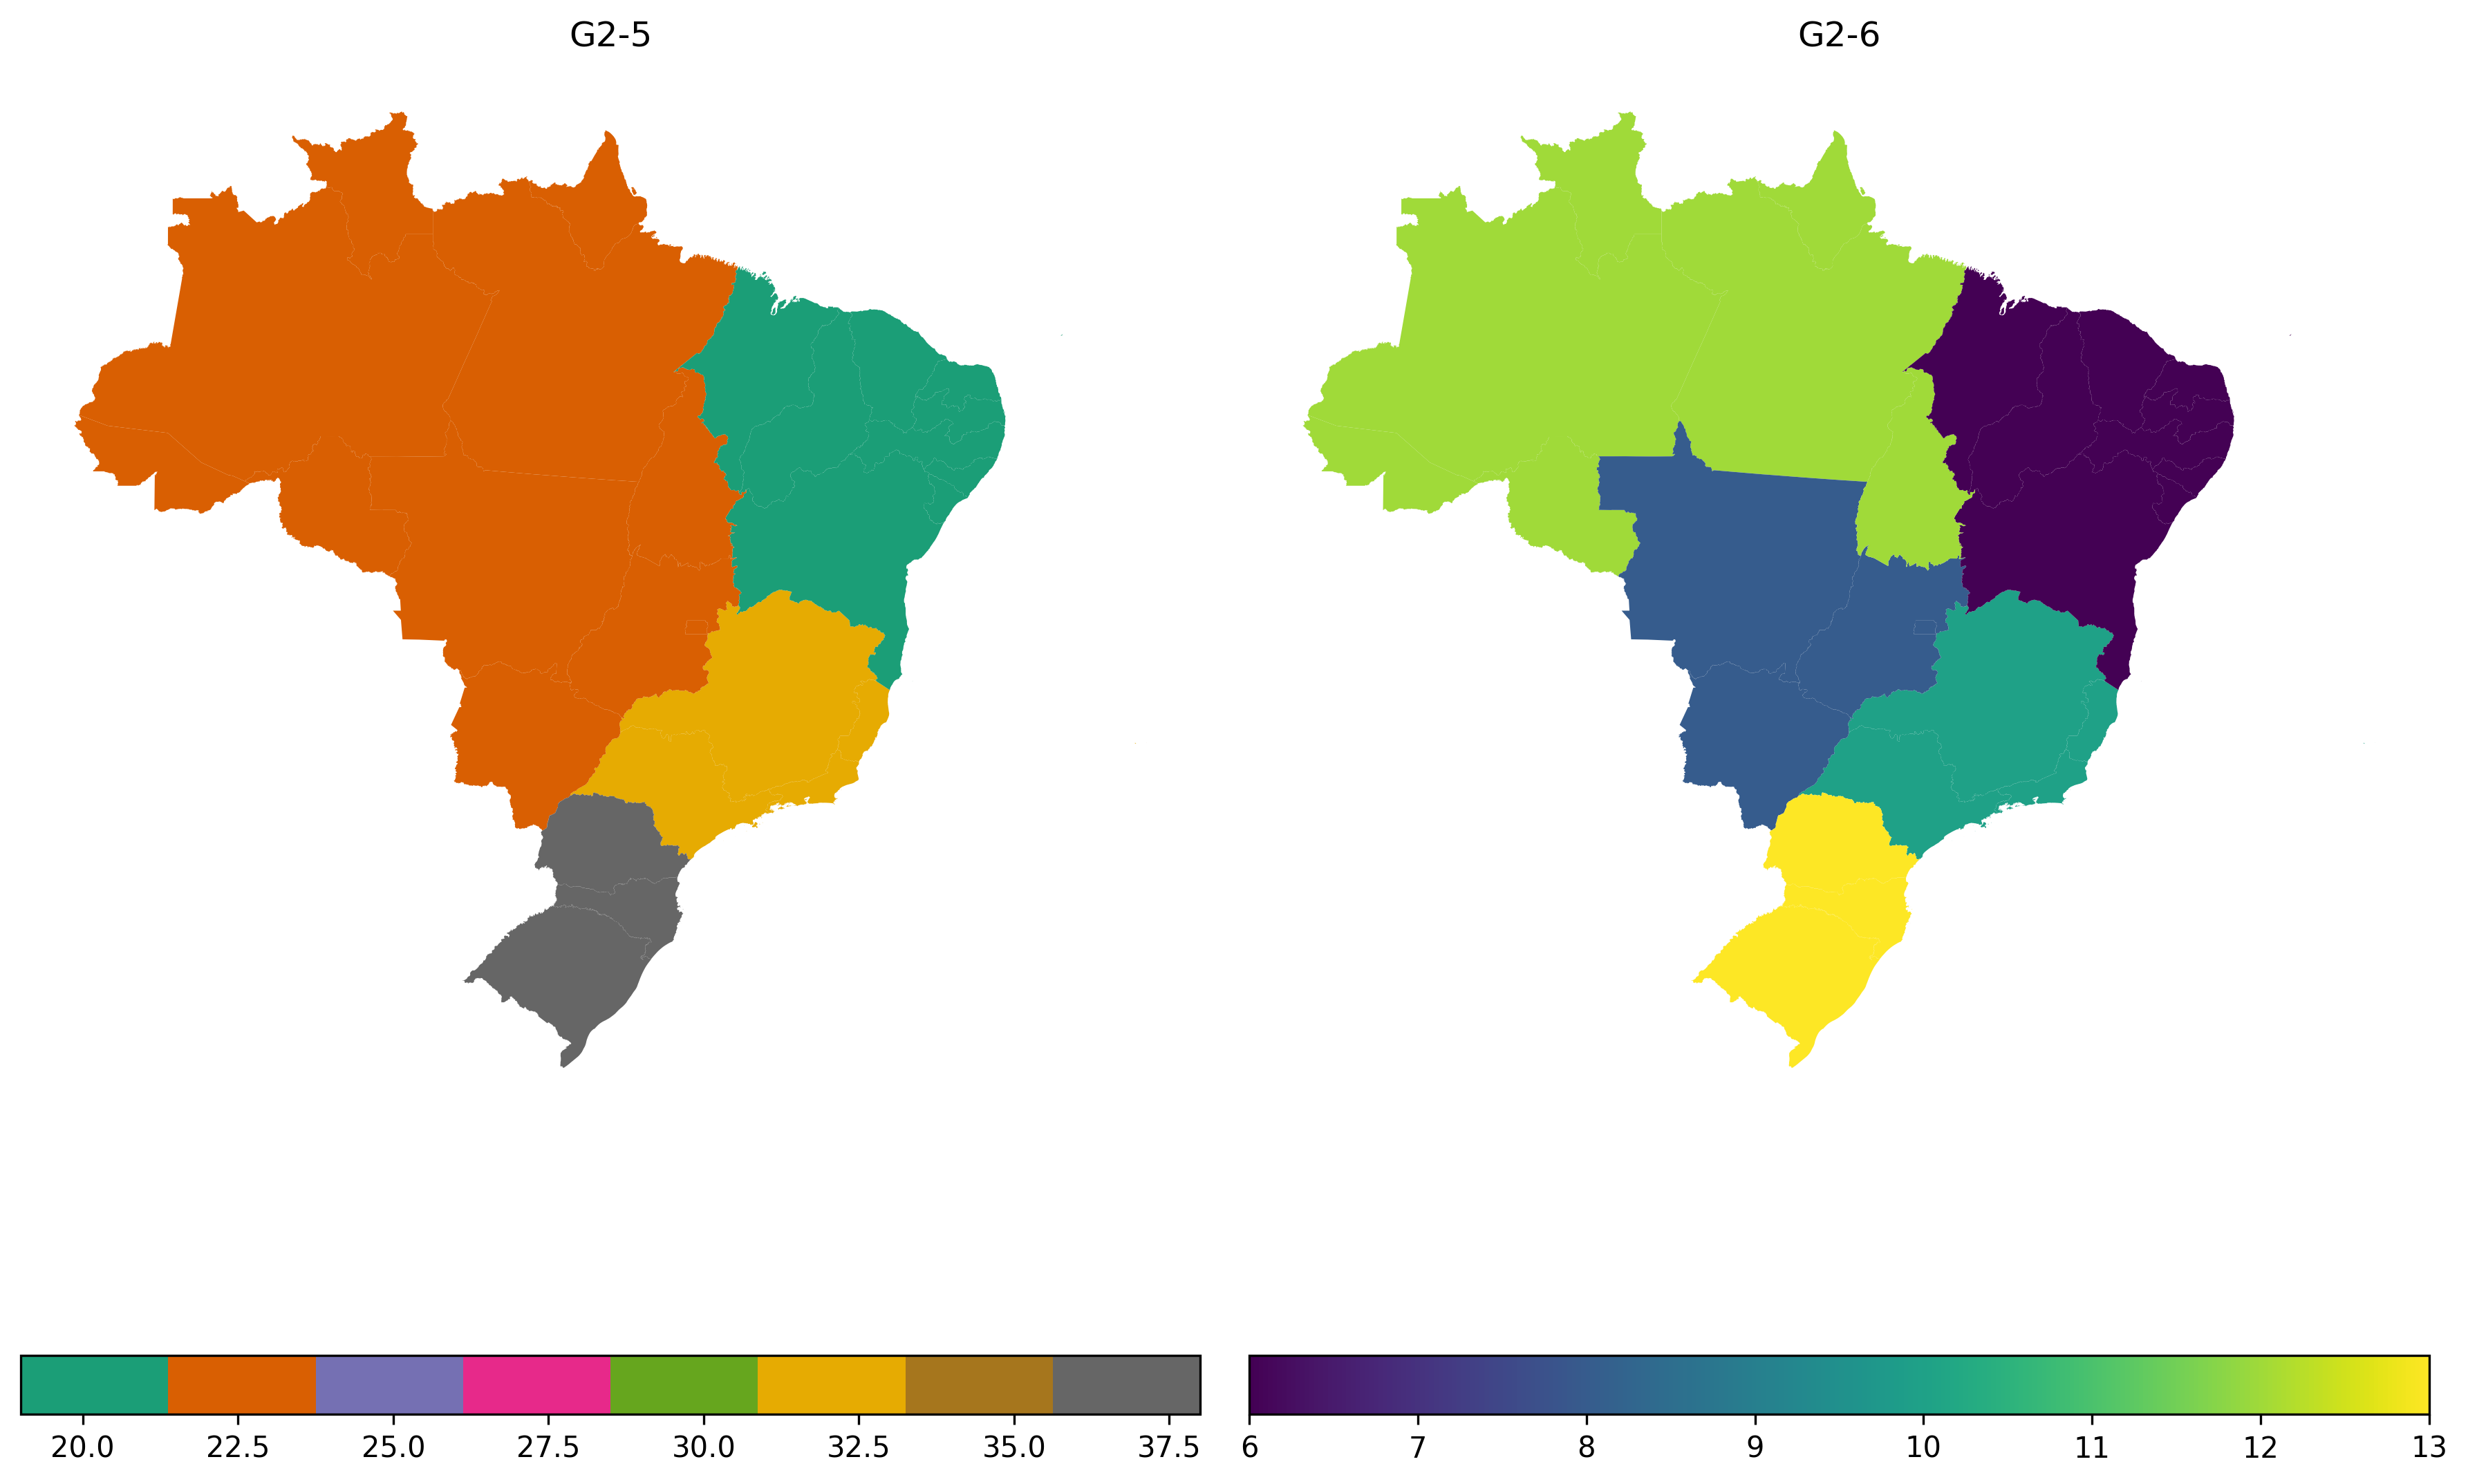
\includegraphics[width=1\linewidth]{figuras/mapa_coropletico_tic_domicilios_2024_g2_5_6.png}
	\label{fig:mapa_coropletico_tic_domicilios_2024_g2_5_6}
	\footnotesize{Fonte: \cite{tic_domicilios_2024_g2}.}
\end{figure}

Quando se trata do indicador G2-5, apenas as regiões Sudeste e Sul foram as que mais usaram serviços públicos relativos a impostos e taxas governamentais, como declaração de imposto de renda, IPVA ou IPTU.

Quando se trata do indicador G2-6, apenas a região Sul foi a que mais usou serviços públicos relativos à polícia e segurança, como boletim de ocorrência, antecedentes criminais ou denúncias.

\begin{figure}[H]
	\centering
	\caption{Indicador G2: critério 7 (em \%)}
	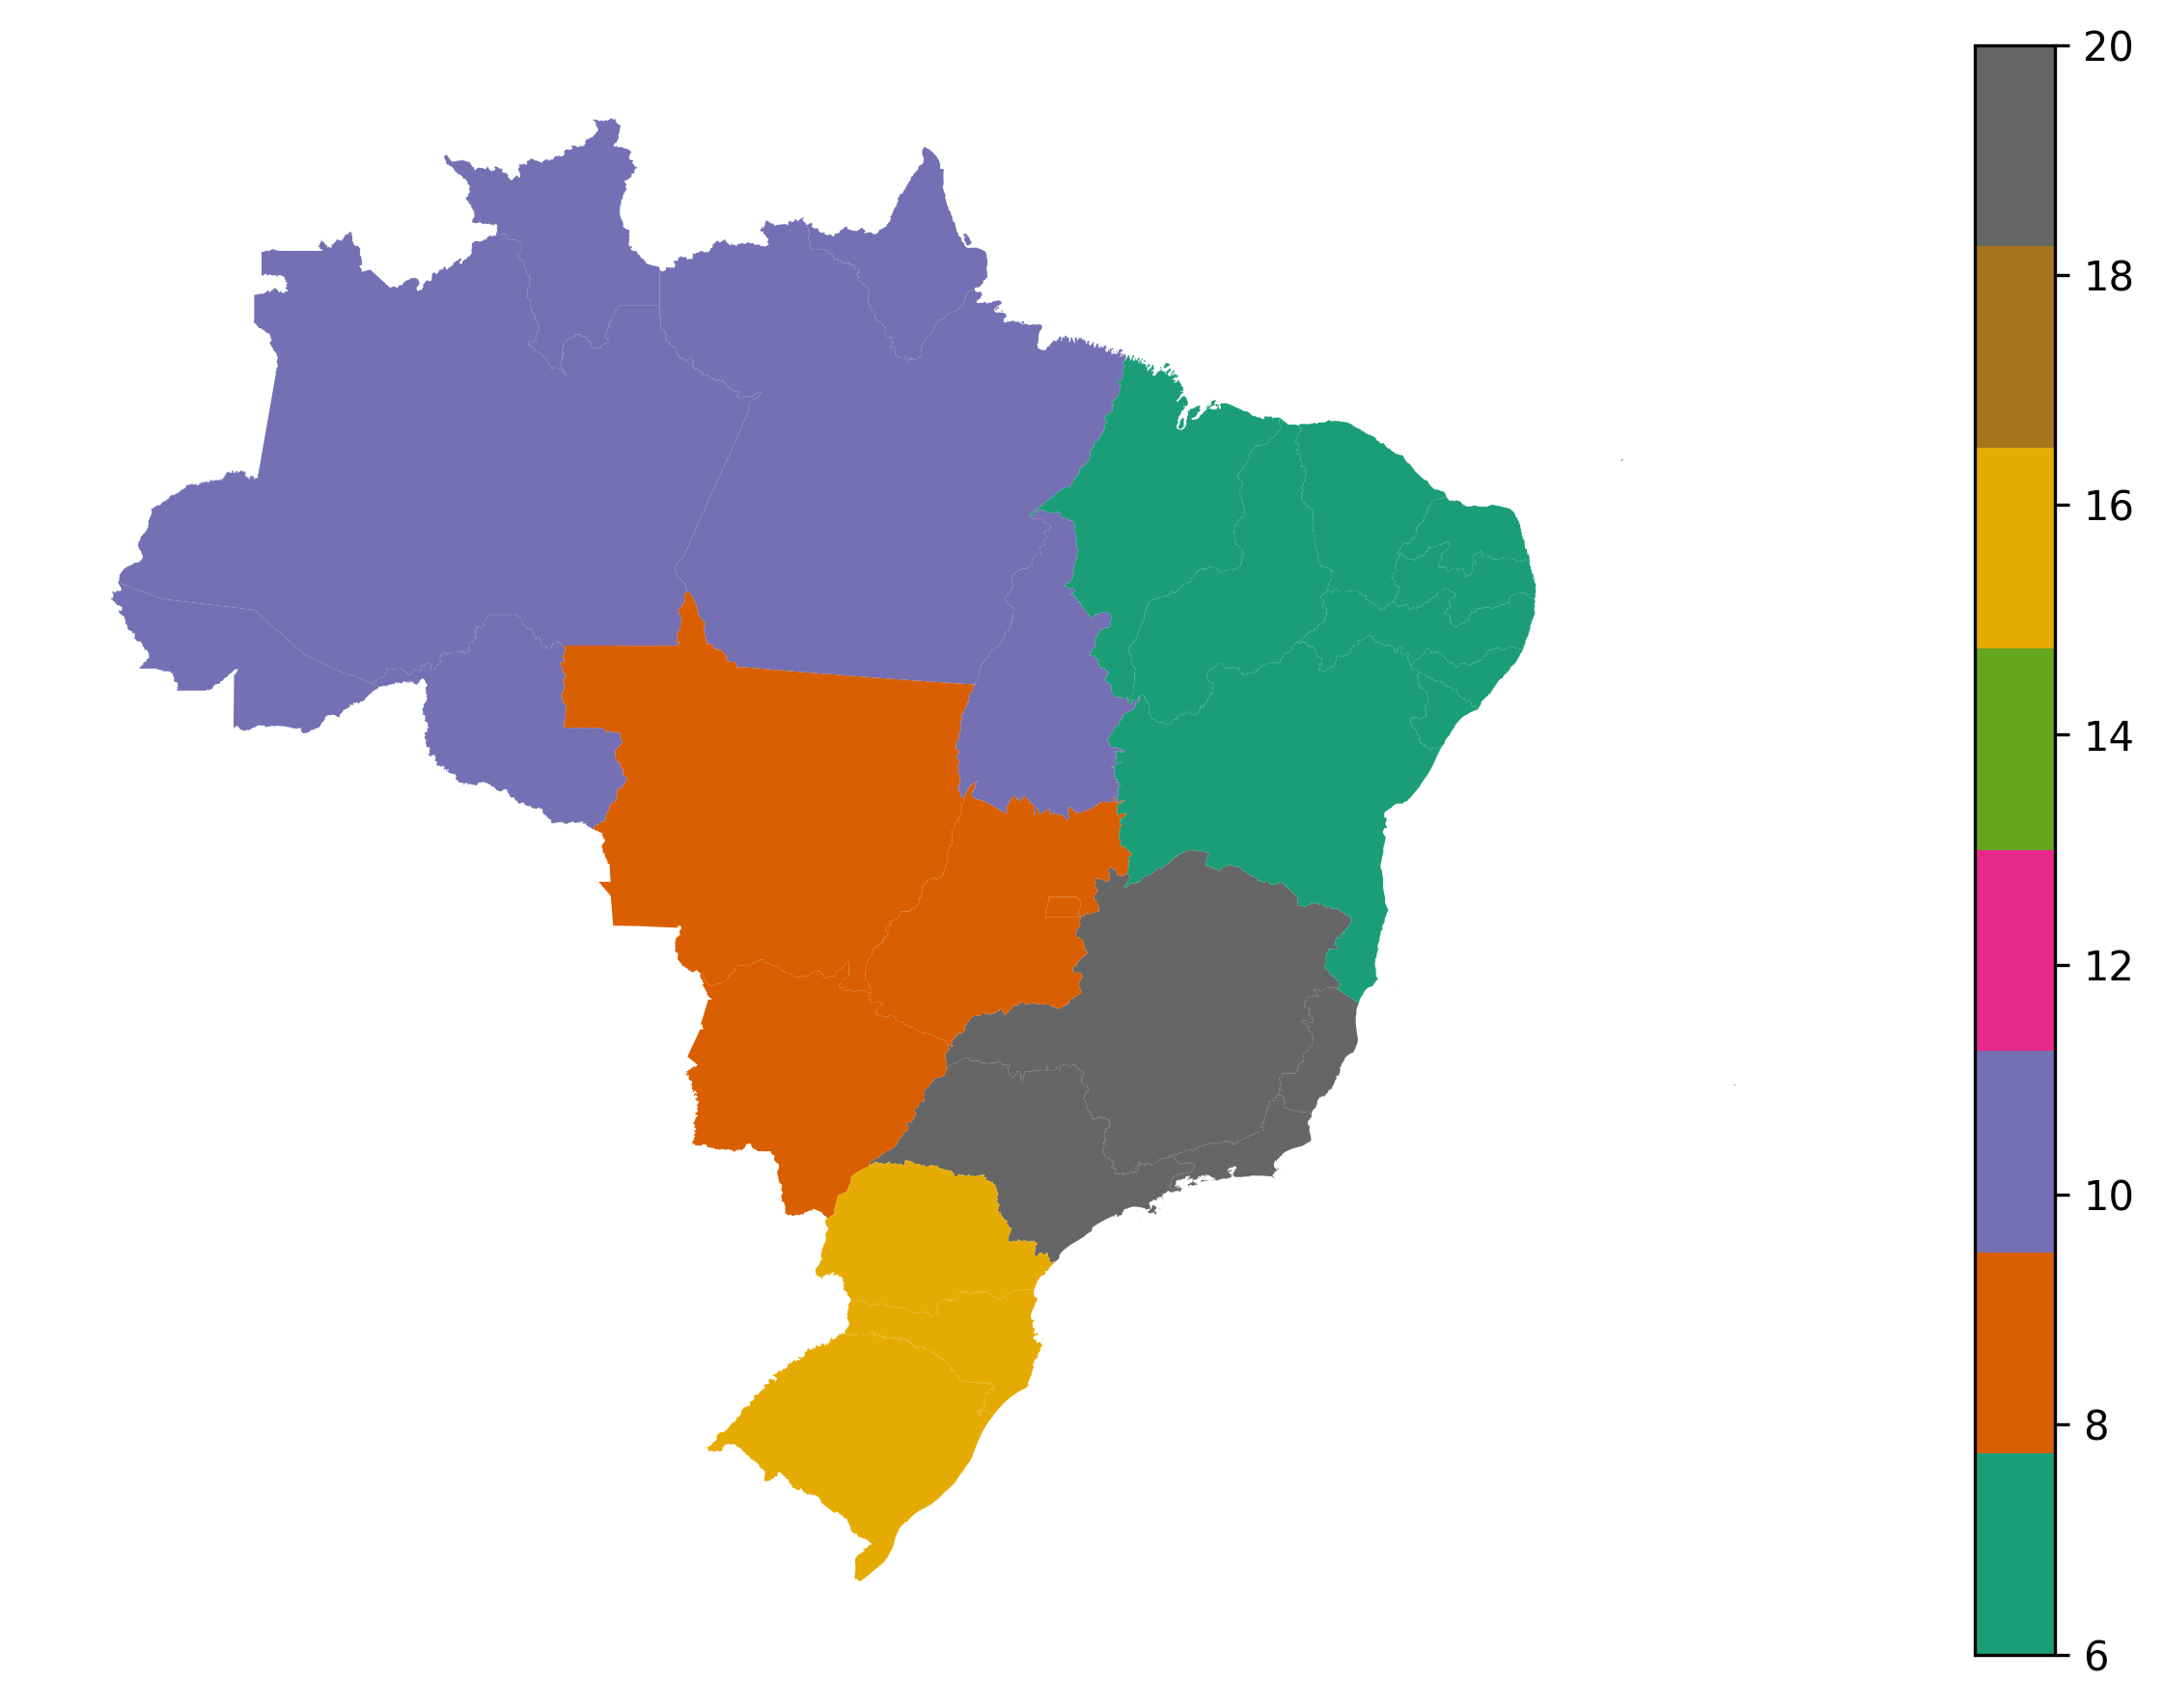
\includegraphics[width=1\linewidth]{figuras/mapa_coropletico_tic_domicilios_2024_g2_7.png}
	\label{fig:mapa_coropletico_tic_domicilios_2024_g2_7}
	\footnotesize{Fonte: \cite{tic_domicilios_2024_g2}.}
\end{figure}

Quando se trata do indicador G2-7, as regiões Sudeste e Sul foram as únicas que mais usaram serviços públicos relativos a transporte público ou outros serviços urbanos, como limpeza e conservação de vias e iluminação.

Complementar ao indicador G2, o indicador G2A detalha se o serviço público foi realizado, completamente ou parcialmente, na internet, e se apenas informações do serviço público foram procuradas na internet, incluídas as opções em que o questionado não respondeu ou não sabe, todos como subcritérios. 

O indicador G2A tem 7 critérios, conforme exposto abaixo:

\begin{itemize}
	\item Documentos pessoais, como RG, CPF, passaporte ou carteira de trabalho.
	Saúde pública, como agendamento de consultas, remédios ou outros serviços do sistema público de saúde.
	\item Educação pública, como Enem, Prouni, matrículas em escolas ou universidades públicas.
	\item Direito do trabalhador ou previdência social, como INSS, FGTS, seguro-desemprego, auxílio-doença ou aposentadoria.
	\item Impostos e taxas governamentais, como declaração de imposto de renda, IPVA ou IPTU.
	\item Polícia e segurança, como boletim de ocorrência, antecedentes criminais ou denúncias.
	\item Transporte público ou outros serviços urbanos, como limpeza e conservação de vias, iluminação.
\end{itemize}

Os subcritérios do indicador G2A são, segundo \cite{tic_domicilios_2024_g2a}:

\begin{itemize}
    \item Realizou serviço na Internet sem precisar ir até um posto (SC1);  \item Realizou parte do serviço na Internet, mas precisou ir a um posto para finalizar (SC2);
    \item Apenas procurou informações na Internet (SC3);
    \item Não sabe; e
    \item Não respondeu.
\end{itemize}

As figuras \ref{fig:mapa_coropletico_tic_domicilios_2024_g2a_1}, \ref{fig:mapa_coropletico_tic_domicilios_2024_g2a_2}, \ref{fig:mapa_coropletico_tic_domicilios_2024_g2a_3},
\ref{fig:mapa_coropletico_tic_domicilios_2024_g2a_4},
\ref{fig:mapa_coropletico_tic_domicilios_2024_g2a_5} contêm mapa coropléticos que demonstram os subcritérios dos indicadores do G2A, que não incluirão as opções \textbf{não respondeu} e \textbf{não sabe}.

\begin{figure}[H]
	\centering
	\caption{Indicador G2A: critério 1 (em \%)}
	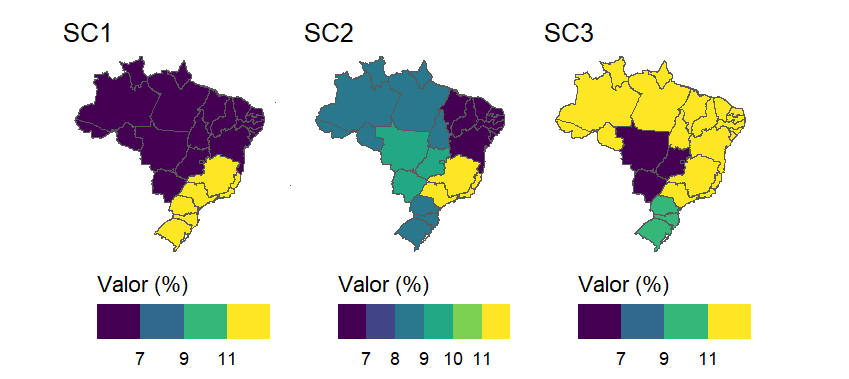
\includegraphics[width=1\linewidth]{figuras/mapa_coropletico_tic_domicilios_2024_g2a_1.png}
	\label{fig:mapa_coropletico_tic_domicilios_2024_g2a_1}
	\footnotesize{Fonte: \cite{tic_domicilios_2024_g2a}.}
\end{figure}

No tocante ao SC1, as regiões Sudeste e Sul foram as regiões em que mais ocorreram serviços na internet sem precisar ir até um posto. 

No tocante ao SC2, a região Sudeste foi a única região em que mais foram realizados partes dos serviços na Internet, mas foi preciso ir a um posto para finalizar, seguida do Centro-Oeste e das regiões Norte e Sul.

No tocante ao SC3, as regiões Norte, Nordeste, Sudeste foram as regiões em que mais se procurou informações na internet, seguidas do Sul e do Centro-Oeste.

\begin{figure}[H]
	\centering
	\caption{Indicador G2A: critério 2 (em \%)}
	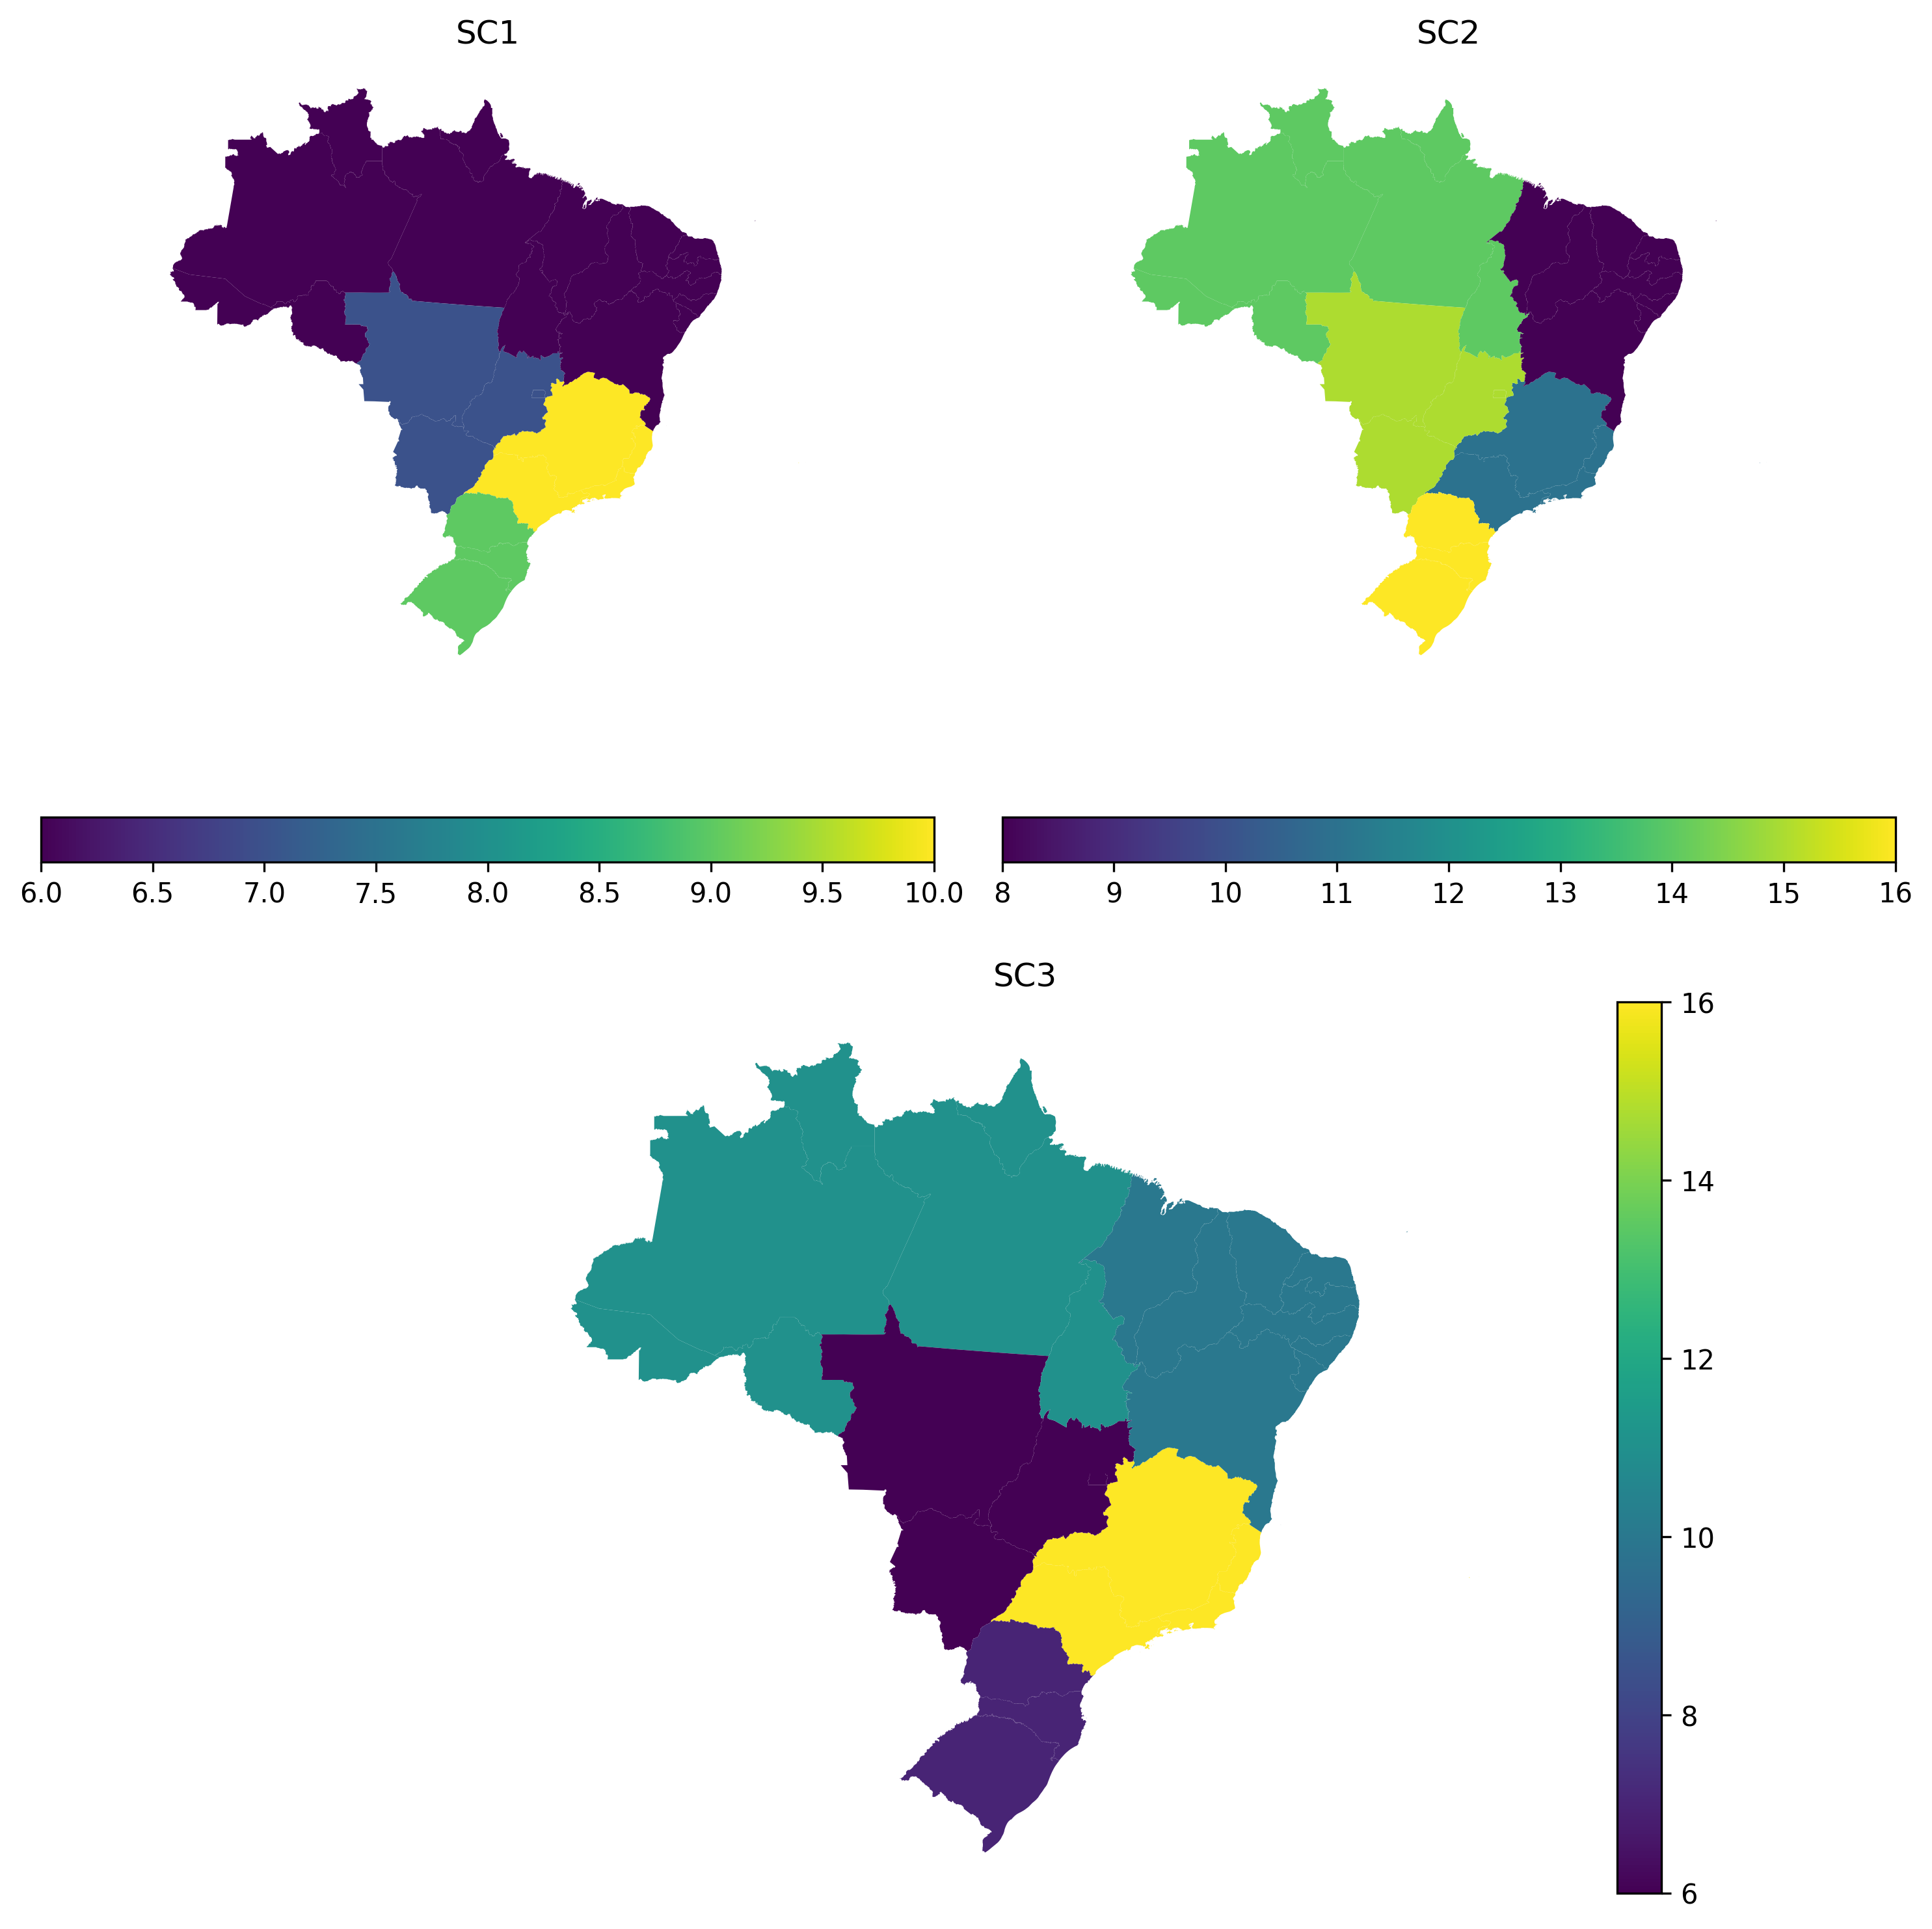
\includegraphics[width=1\linewidth]{figuras/mapa_coropletico_tic_domicilios_2024_g2a_2.png}
	\label{fig:mapa_coropletico_tic_domicilios_2024_g2a_2}
	\footnotesize{Fonte: \cite{tic_domicilios_2024_g2a}.}
\end{figure}

No tocante ao SC1, as regiões Sudeste e Sul foram as regiões em que mais ocorreram serviços na internet sem precisar ir até um posto.

No tocante ao SC2, a região Sudeste foi a região em que mais foram realizados partes dos serviços na Internet, mas foi preciso ir a um posto para finalizar, seguidas  das regiões Sul e Norte, e por fim, do Centro-Oeste.

No tocante ao SC3, a região Sudeste foi a região em que mais se procurou informações na internet, seguida do Nordeste e Norte, bem como, conjuntamente, o Centro-Oeste e o Sul.

\begin{figure}[H]
	\centering
	\caption{Indicador G2A: critério 3 (em \%)}
	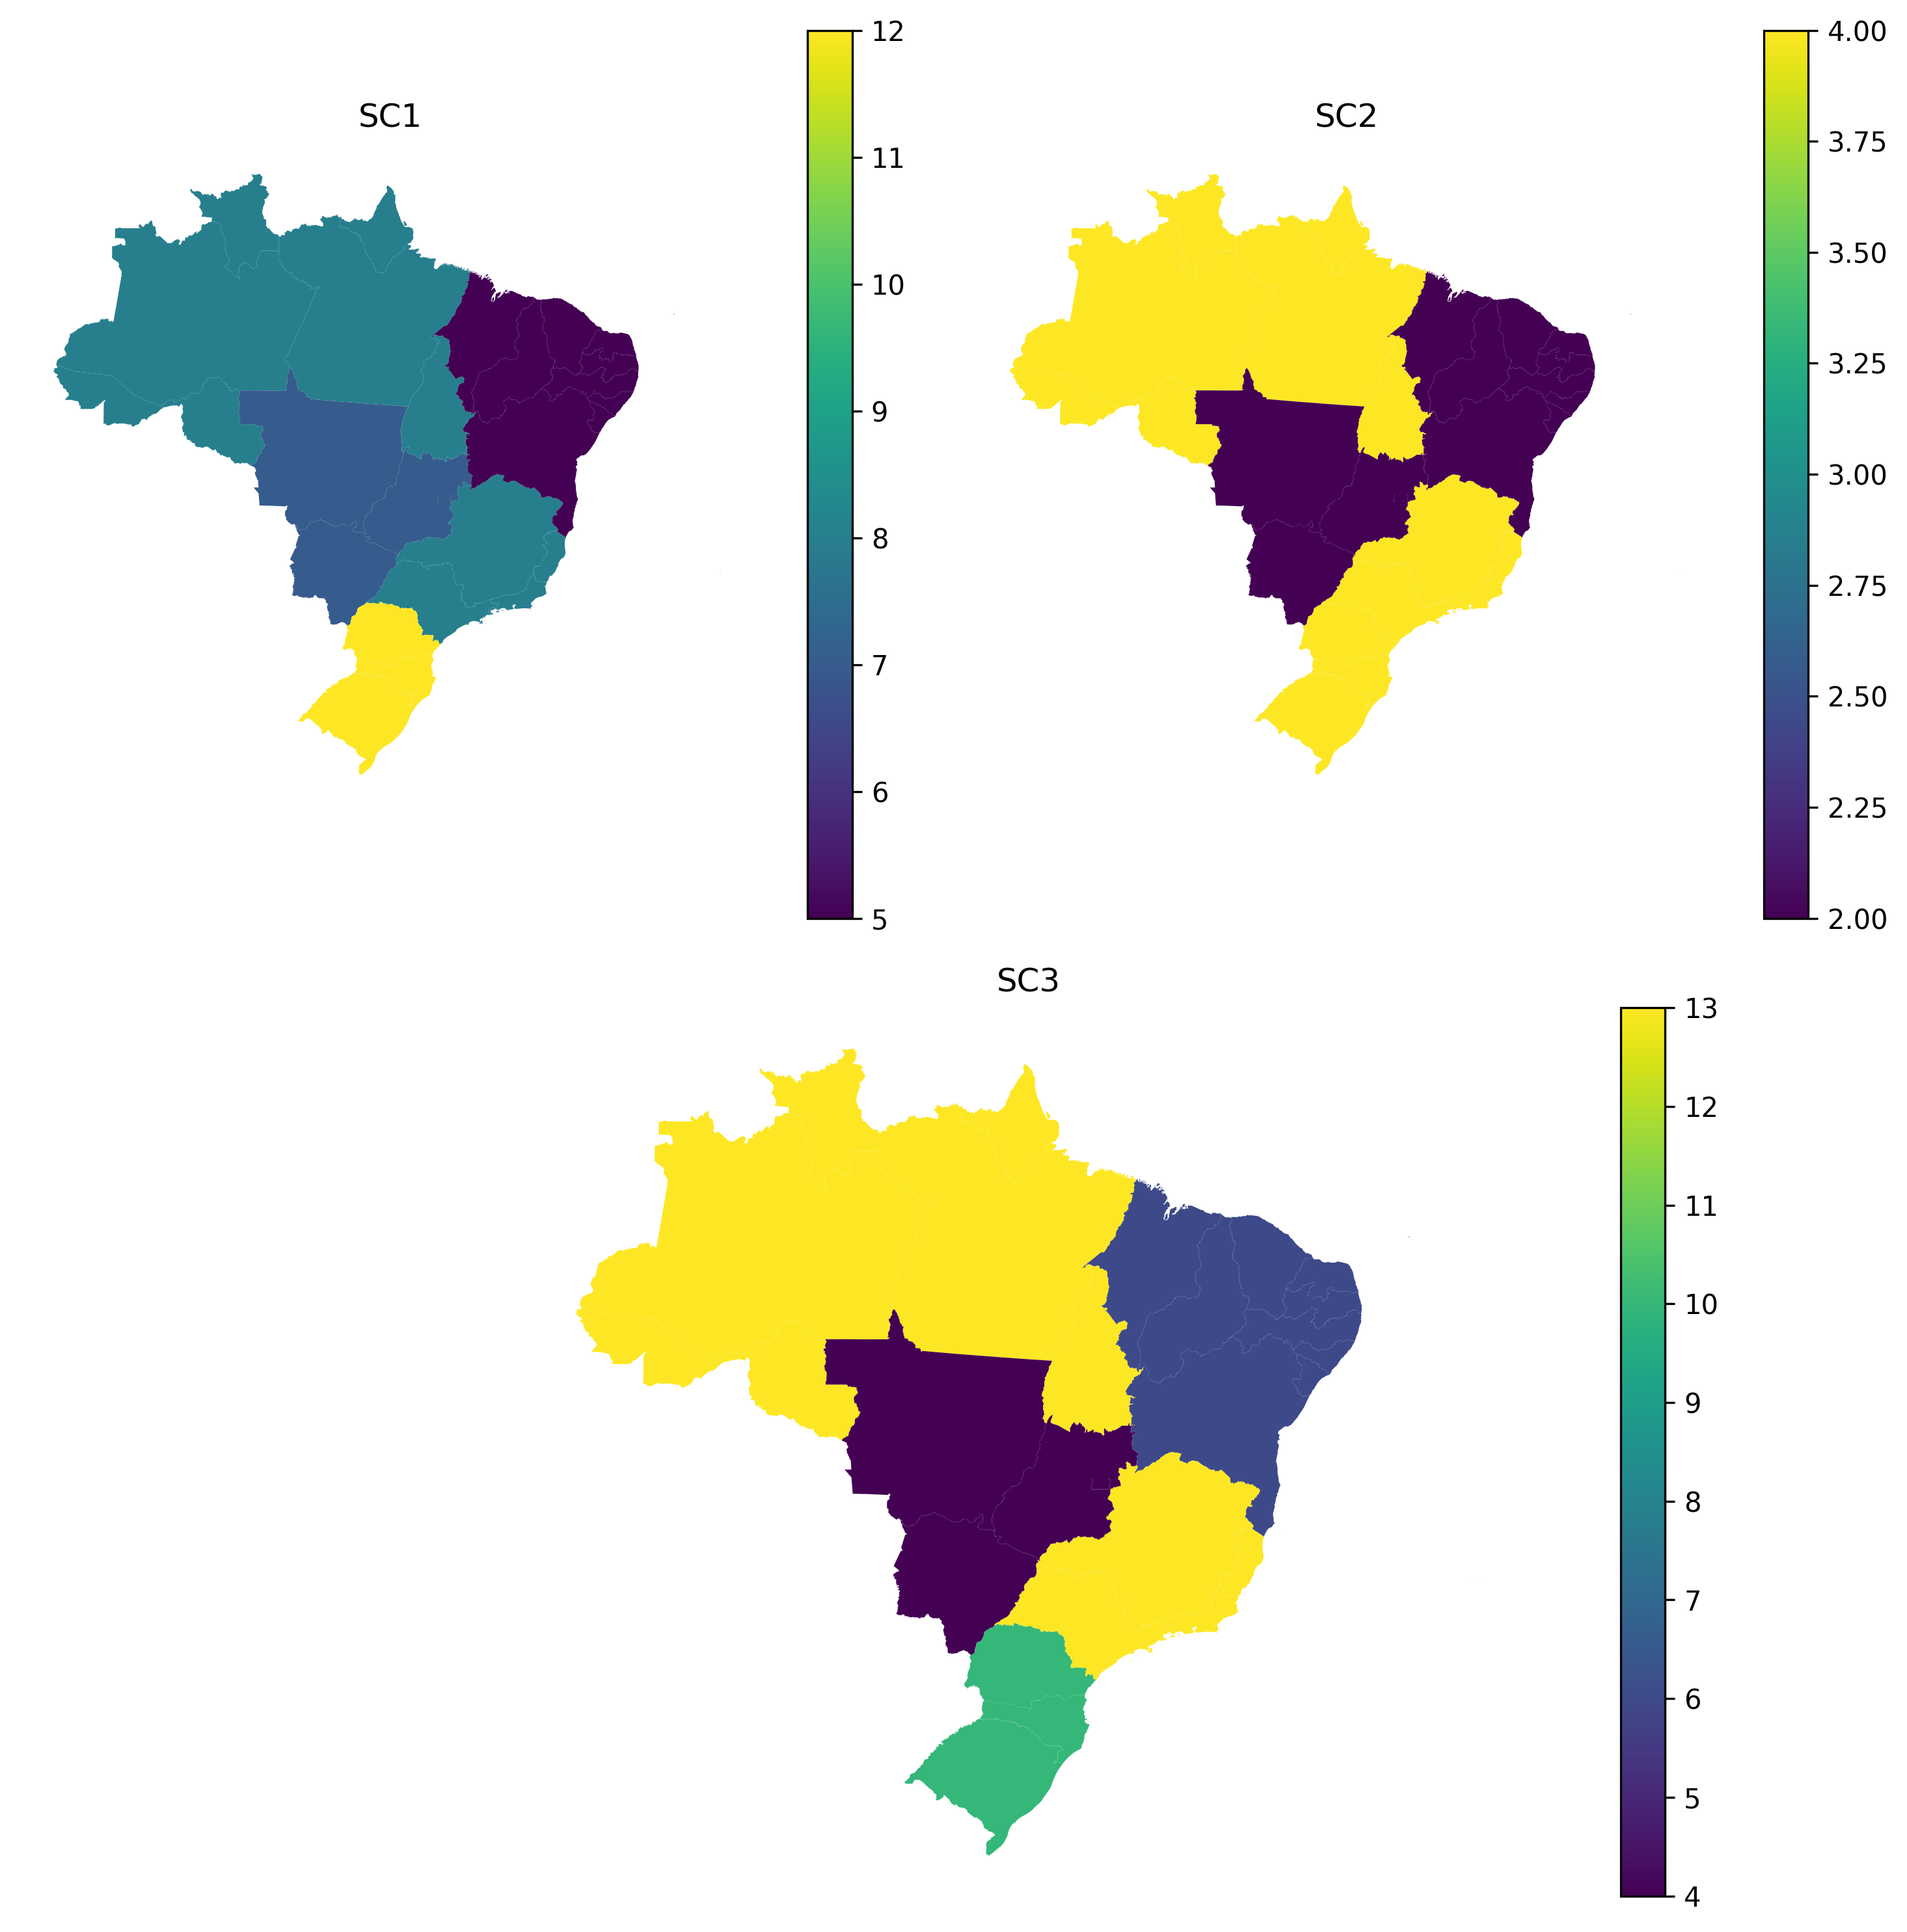
\includegraphics[width=1\linewidth]{figuras/mapa_coropletico_tic_domicilios_2024_g2a_3.png}
	\label{fig:mapa_coropletico_tic_domicilios_2024_g2a_3}
	\footnotesize{Fonte: \cite{tic_domicilios_2024_g2a}.}
\end{figure}

No tocante ao SC1, a região Sul foi a região em que mais ocorreram serviços na internet sem precisar ir até um posto, sendo o Nordeste a região em que mais se foi presencialmente aos postos.

No tocante ao SC2, as regiões Norte, Sudeste e Sul foram as regiões em que mais foram realizados partes dos serviços na Internet, mas foi preciso ir a um posto para finalizar, seguidas do Nordeste e Centro-Oeste.

No tocante ao SC3, as regiões Norte e Sudeste em que mais se procurou informações na internet, seguidas do Nordeste e das regiões Centro-Oeste e Sul.

\begin{figure}[H]
	\centering
	\caption{Indicador G2A: critério 4 (em \%)}
	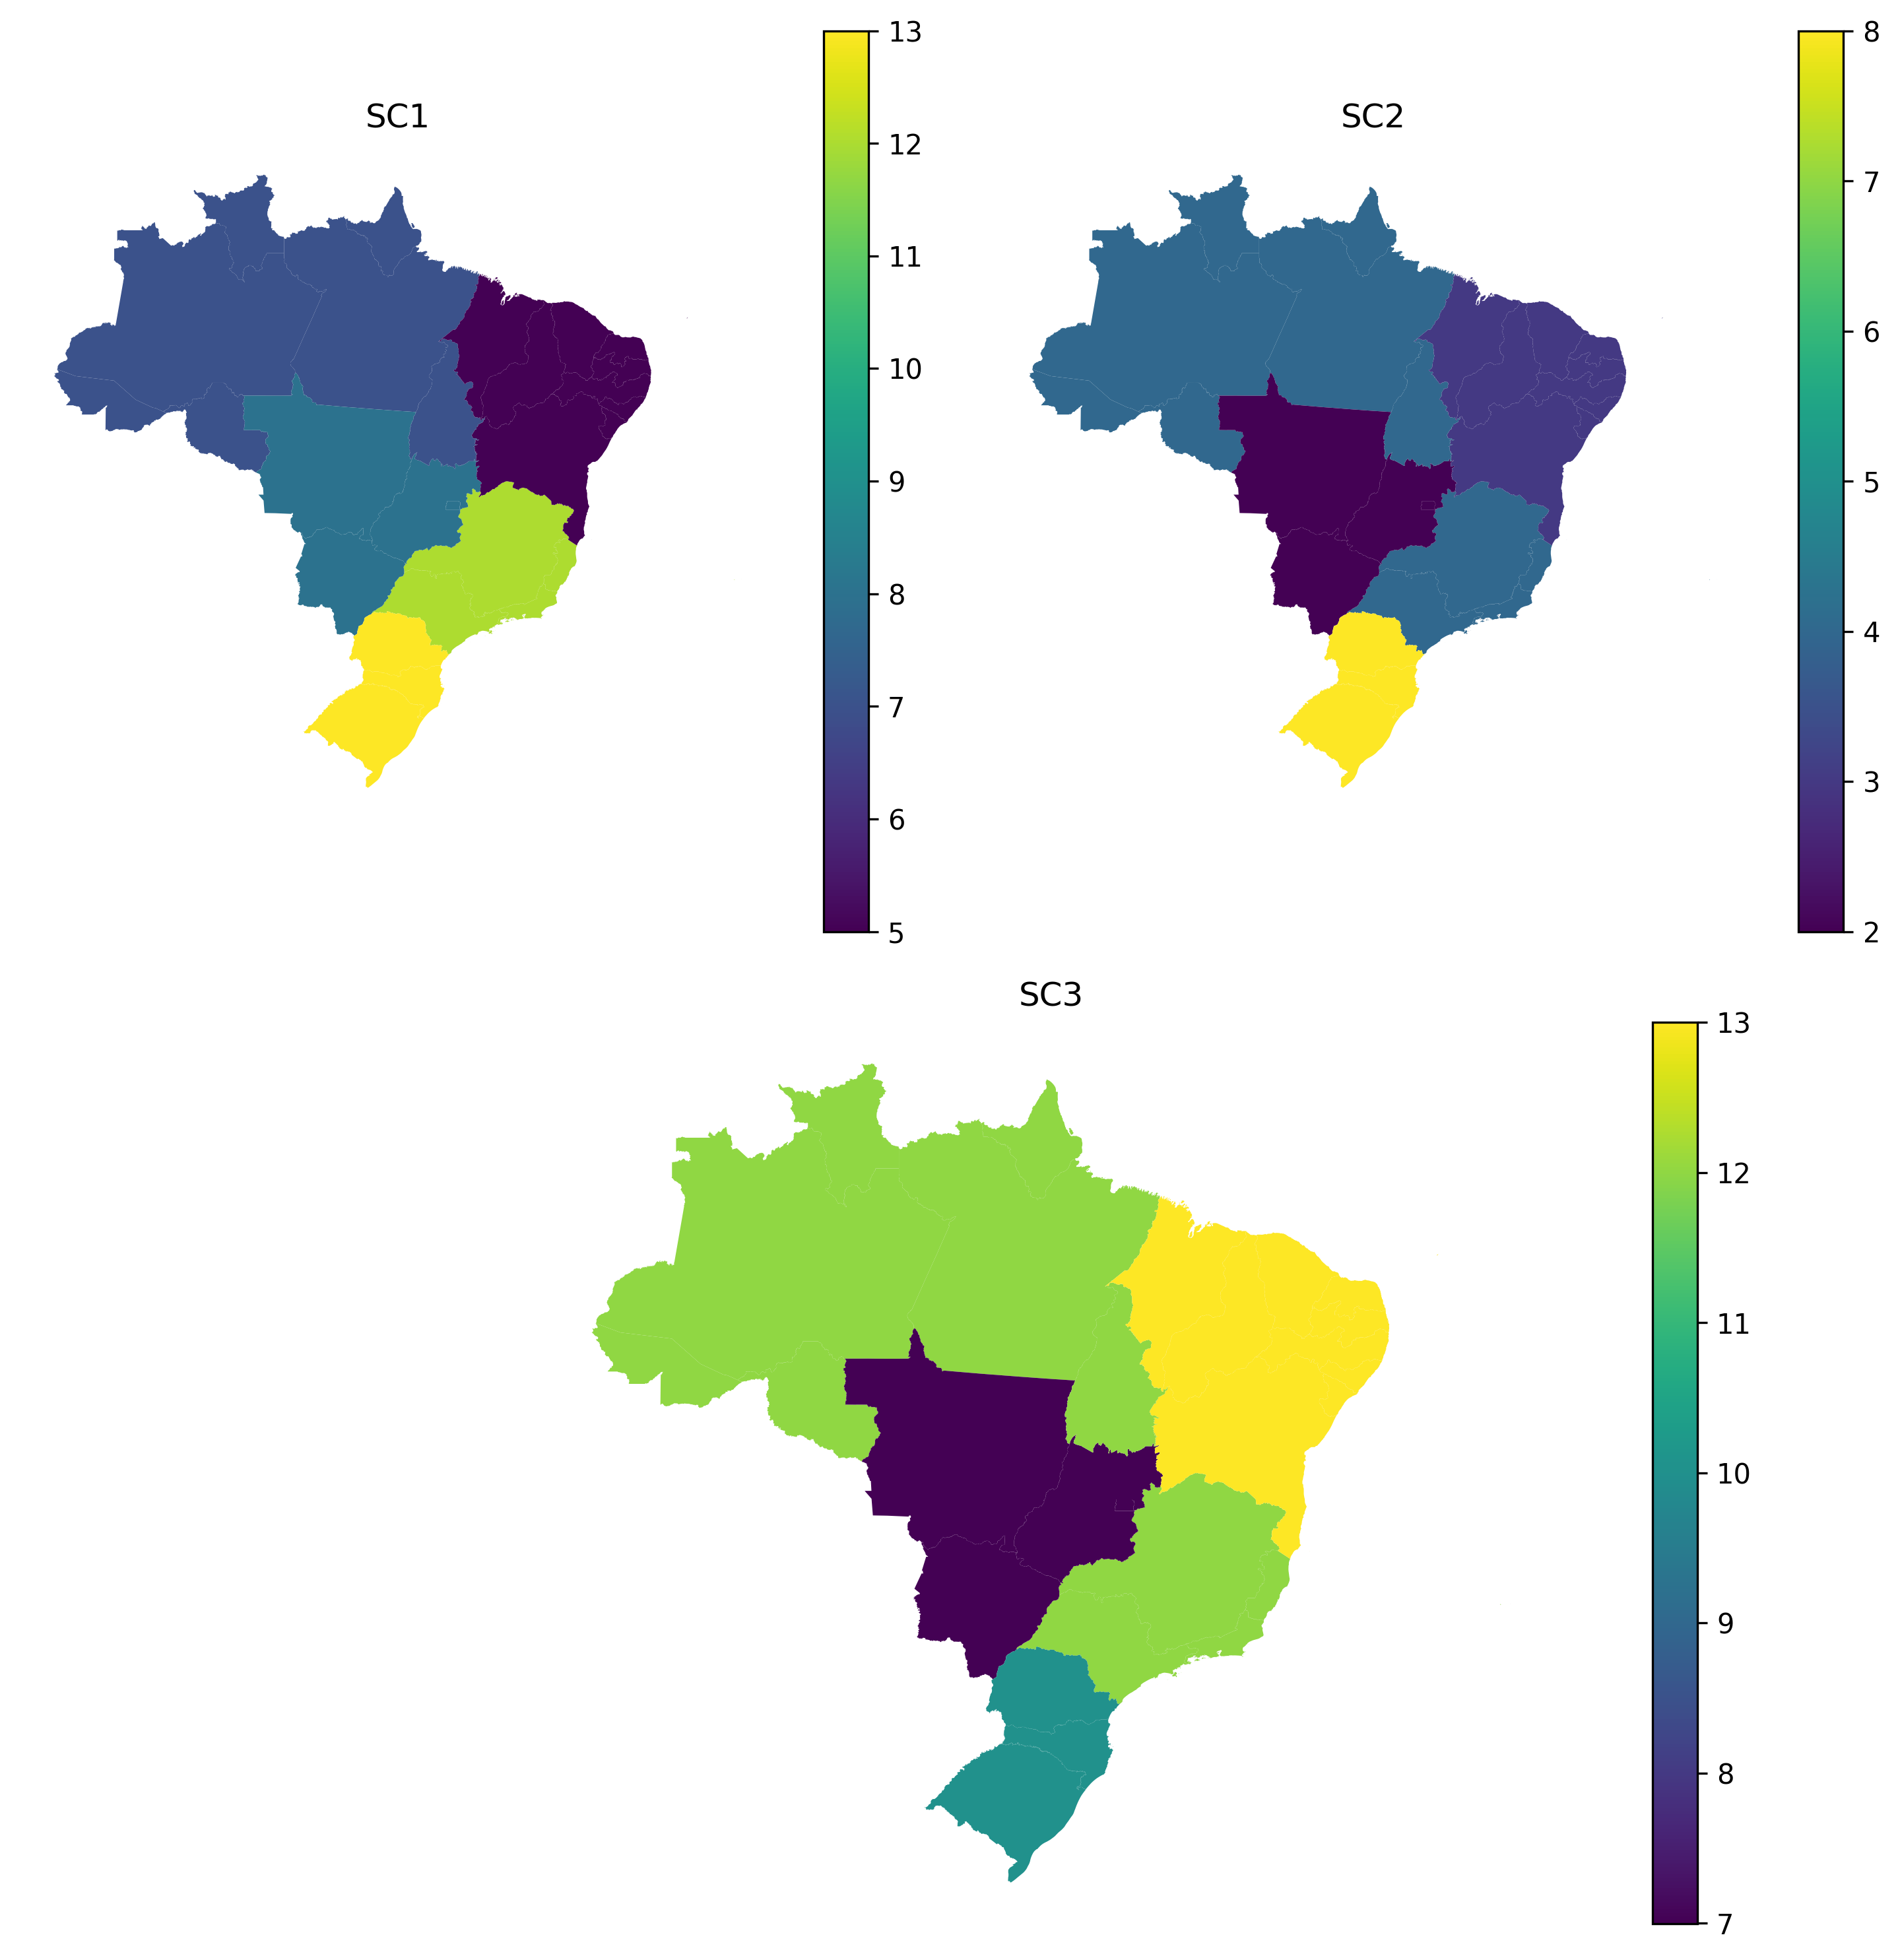
\includegraphics[width=1\linewidth]{figuras/mapa_coropletico_tic_domicilios_2024_g2a_4.png}
	\label{fig:mapa_coropletico_tic_domicilios_2024_g2a_4}
	\footnotesize{Fonte: \cite{tic_domicilios_2024_g2a}.}
\end{figure}

No tocante ao SC1, as regiões Sudeste e Sul foram as regiões em que mais ocorreram serviços na internet sem precisar ir até um posto, seguidas do Centro-Oeste e das regiões Norte e Nordeste.

No tocante ao SC2, a região Sul foi a região em que mais foram realizados partes dos serviços na Internet, mas foi preciso ir a um posto para finalizar, seguidas do Sudeste e Norte e das regiões Centro-Oeste e Nordeste.

No tocante ao SC3, a região Nordeste foi a região em que mais se procurou informações na internet, seguidas do Norte e Sudeste e da região Centro-Oeste.

\begin{figure}[H]
	\centering
	\caption{Indicador G2A: critério 5 (em \%)}
	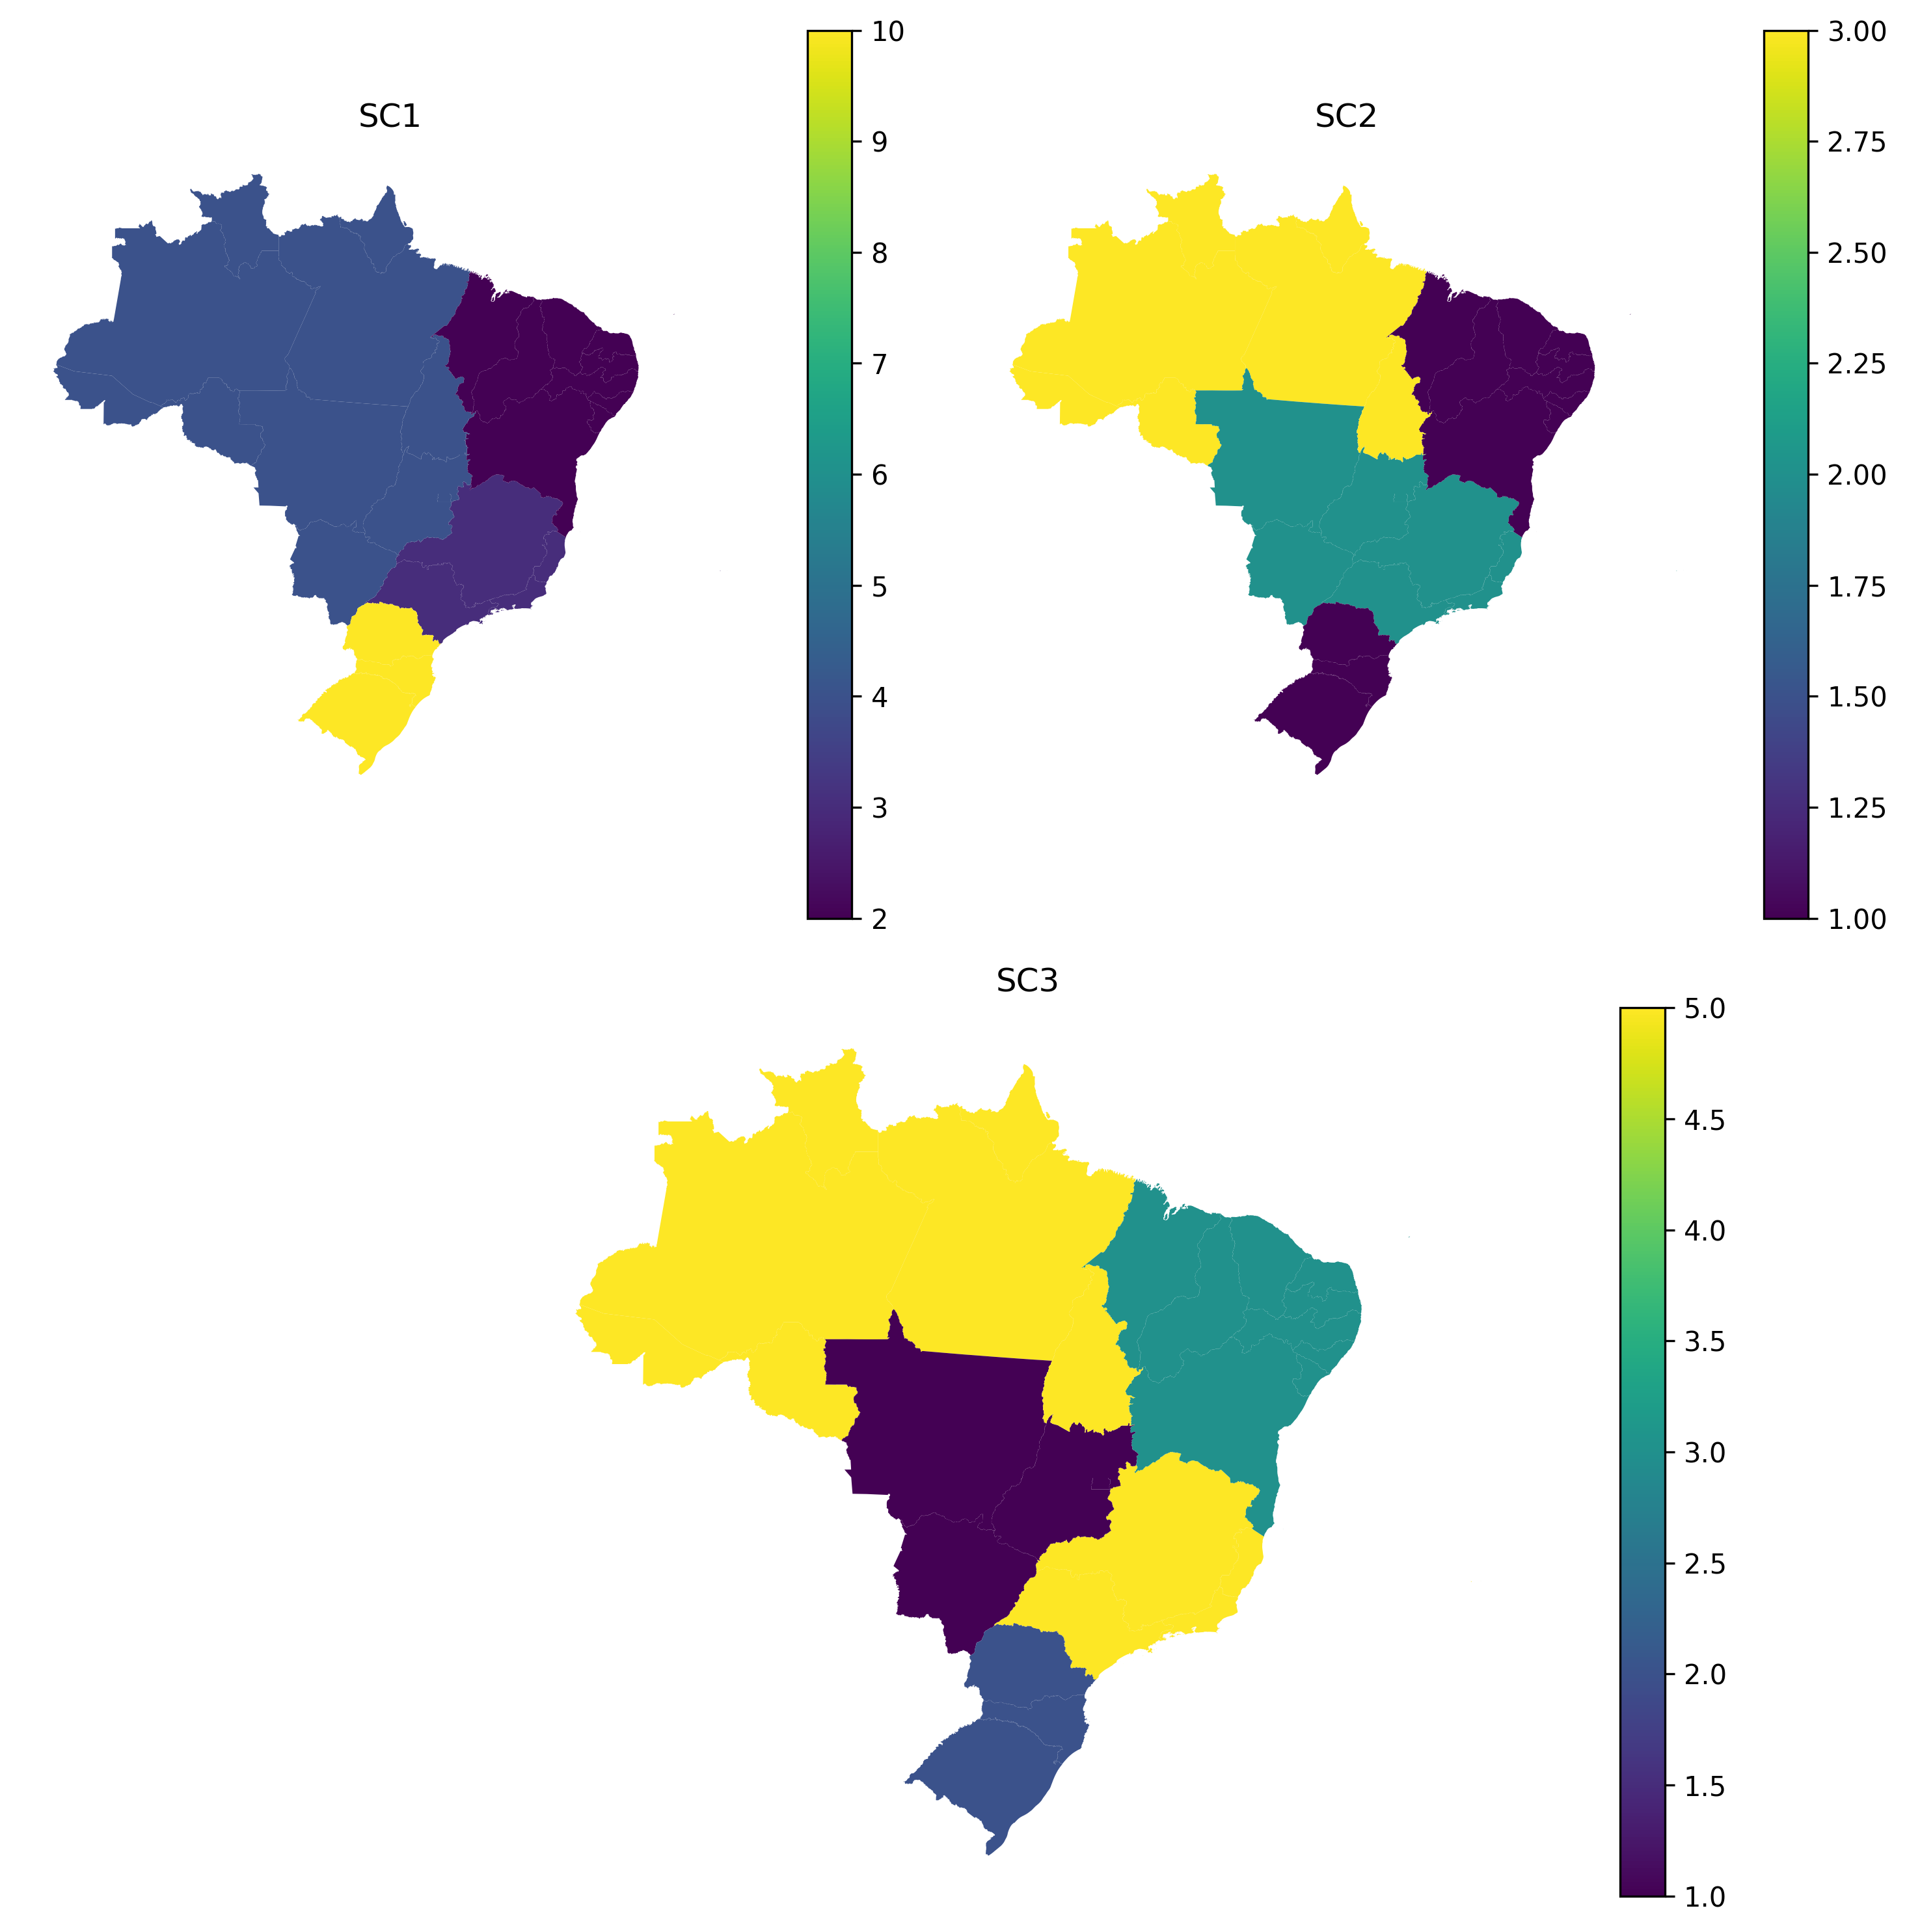
\includegraphics[width=1\linewidth]{figuras/mapa_coropletico_tic_domicilios_2024_g2a_5.png}
	\label{fig:mapa_coropletico_tic_domicilios_2024_g2a_5}
	\footnotesize{Fonte: \cite{tic_domicilios_2024_g2a}.}
\end{figure}

No tocante ao SC1, a região Sul foi a região em que mais ocorreram serviços na internet sem precisar ir até um posto, seguidas do Sudeste, Centro-Oeste e das regiões Norte e Nordeste.

No tocante ao SC2, a região Sul foi a região em que mais foram realizados partes dos serviços na Internet, mas foi preciso ir a um posto para finalizar, seguidas do Centro-Oeste e Norte e das regiões Sudeste e Nordeste.

No tocante ao SC3, as regiões Norte e Nordeste foram a região em que mais se procurou informações na internet, seguidas do Sudeste, Sul e da região Centro-Oeste.

\begin{figure}[H]
	\centering
	\caption{Indicador G2A: critério 6 (em \%)}
	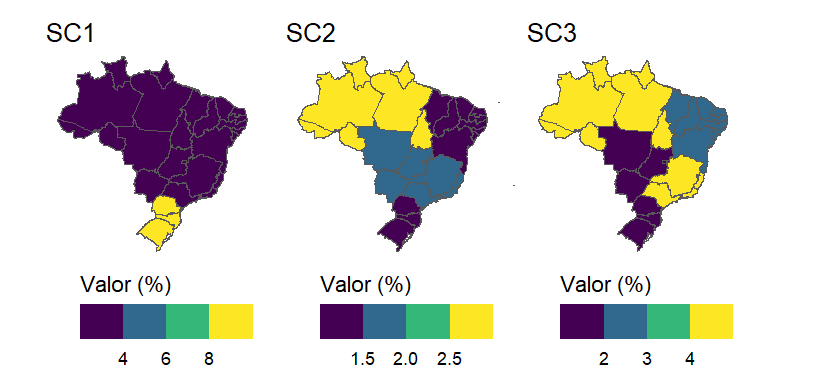
\includegraphics[width=1\linewidth]{figuras/mapa_coropletico_tic_domicilios_2024_g2a_6.png}
	\label{fig:mapa_coropletico_tic_domicilios_2024_g2a_6}
	\footnotesize{Fonte: \cite{tic_domicilios_2024_g2a}.}
\end{figure}

No tocante ao SC1, apenas a região Sul foi a região em que mais ocorreram serviços na internet sem precisar ir até um posto.

No tocante ao SC2, a região Norte foi a região em que mais foram realizados partes dos serviços na Internet, mas foi preciso ir a um posto para finalizar, seguidas do Centro-Oeste e Sudeste e das regiões Sul e Nordeste.

No tocante ao SC3, as regiões Norte e Sudeste foram a região em que mais se procurou informações na internet, seguidas do Nordeste e das regiões Centro-Oeste e Sul.

\begin{figure}[H]
	\centering
	\caption{Indicador G2A: critério 7 (em \%)}
	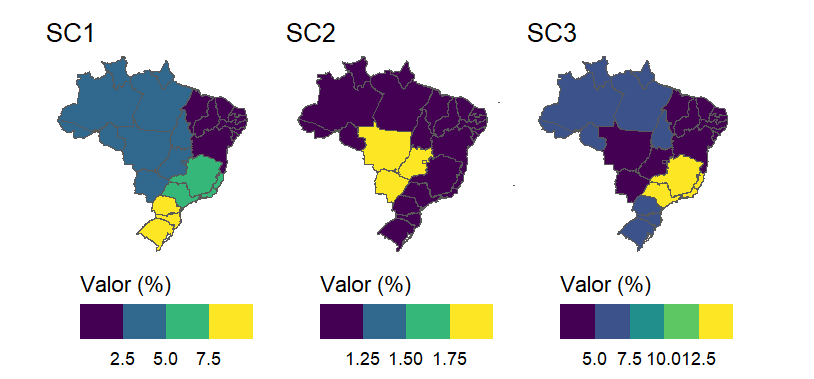
\includegraphics[width=1\linewidth]{figuras/mapa_coropletico_tic_domicilios_2024_g2a_7.png}
	\label{fig:mapa_coropletico_tic_domicilios_2024_g2a_7}
	\footnotesize{Fonte: \cite{tic_domicilios_2024_g2a}.}
\end{figure}

No tocante ao SC1, a região Sul foi a região em que mais ocorreram serviços na internet sem precisar ir até um posto, seguidas das regiões Sudeste, conjuntamente, o Centro-Oeste e o Norte, e por fim, o Nordeste.

No tocante ao SC2, apenas a região Centro-Oeste foi a região em que mais foram realizados partes dos serviços na Internet.

No tocante ao SC3, as regiões Norte e Sudeste foram a região em que mais se procurou informações na internet, seguidas do Nordeste e das regiões Centro-Oeste e Sul.

Terminando a análise do TIC Domicílios 2024, analisar-se-á o indicador G3. O indicador representa os usuários de internet, por atividades de interação com autoridades públicas.

A lista abaixo contém a tabela com a descrição dos seus 3 critérios.  

\begin{itemize}
	\item Procurou informações oferecidas por sites de governo (C1).
	\item Realizou algum serviço público, como emitir documentos pela Internet, preencher e enviar formulários online ou pagar taxas e impostos pela Internet (C2).
	\item Não utilizou a Internet para realizar atividades de interação com autoridades públicas (C3).
\end{itemize}

Haja vista a lista acima, a figura \ref{fig:mapa_coropletico_tic_domicilios_2024_g3}  representa o percentual de usuários de internet, por atividades de interação com autoridades públicas. 

\begin{figure}[H]
	\centering
	\caption{Indicador G3: critérios (em \%)}
	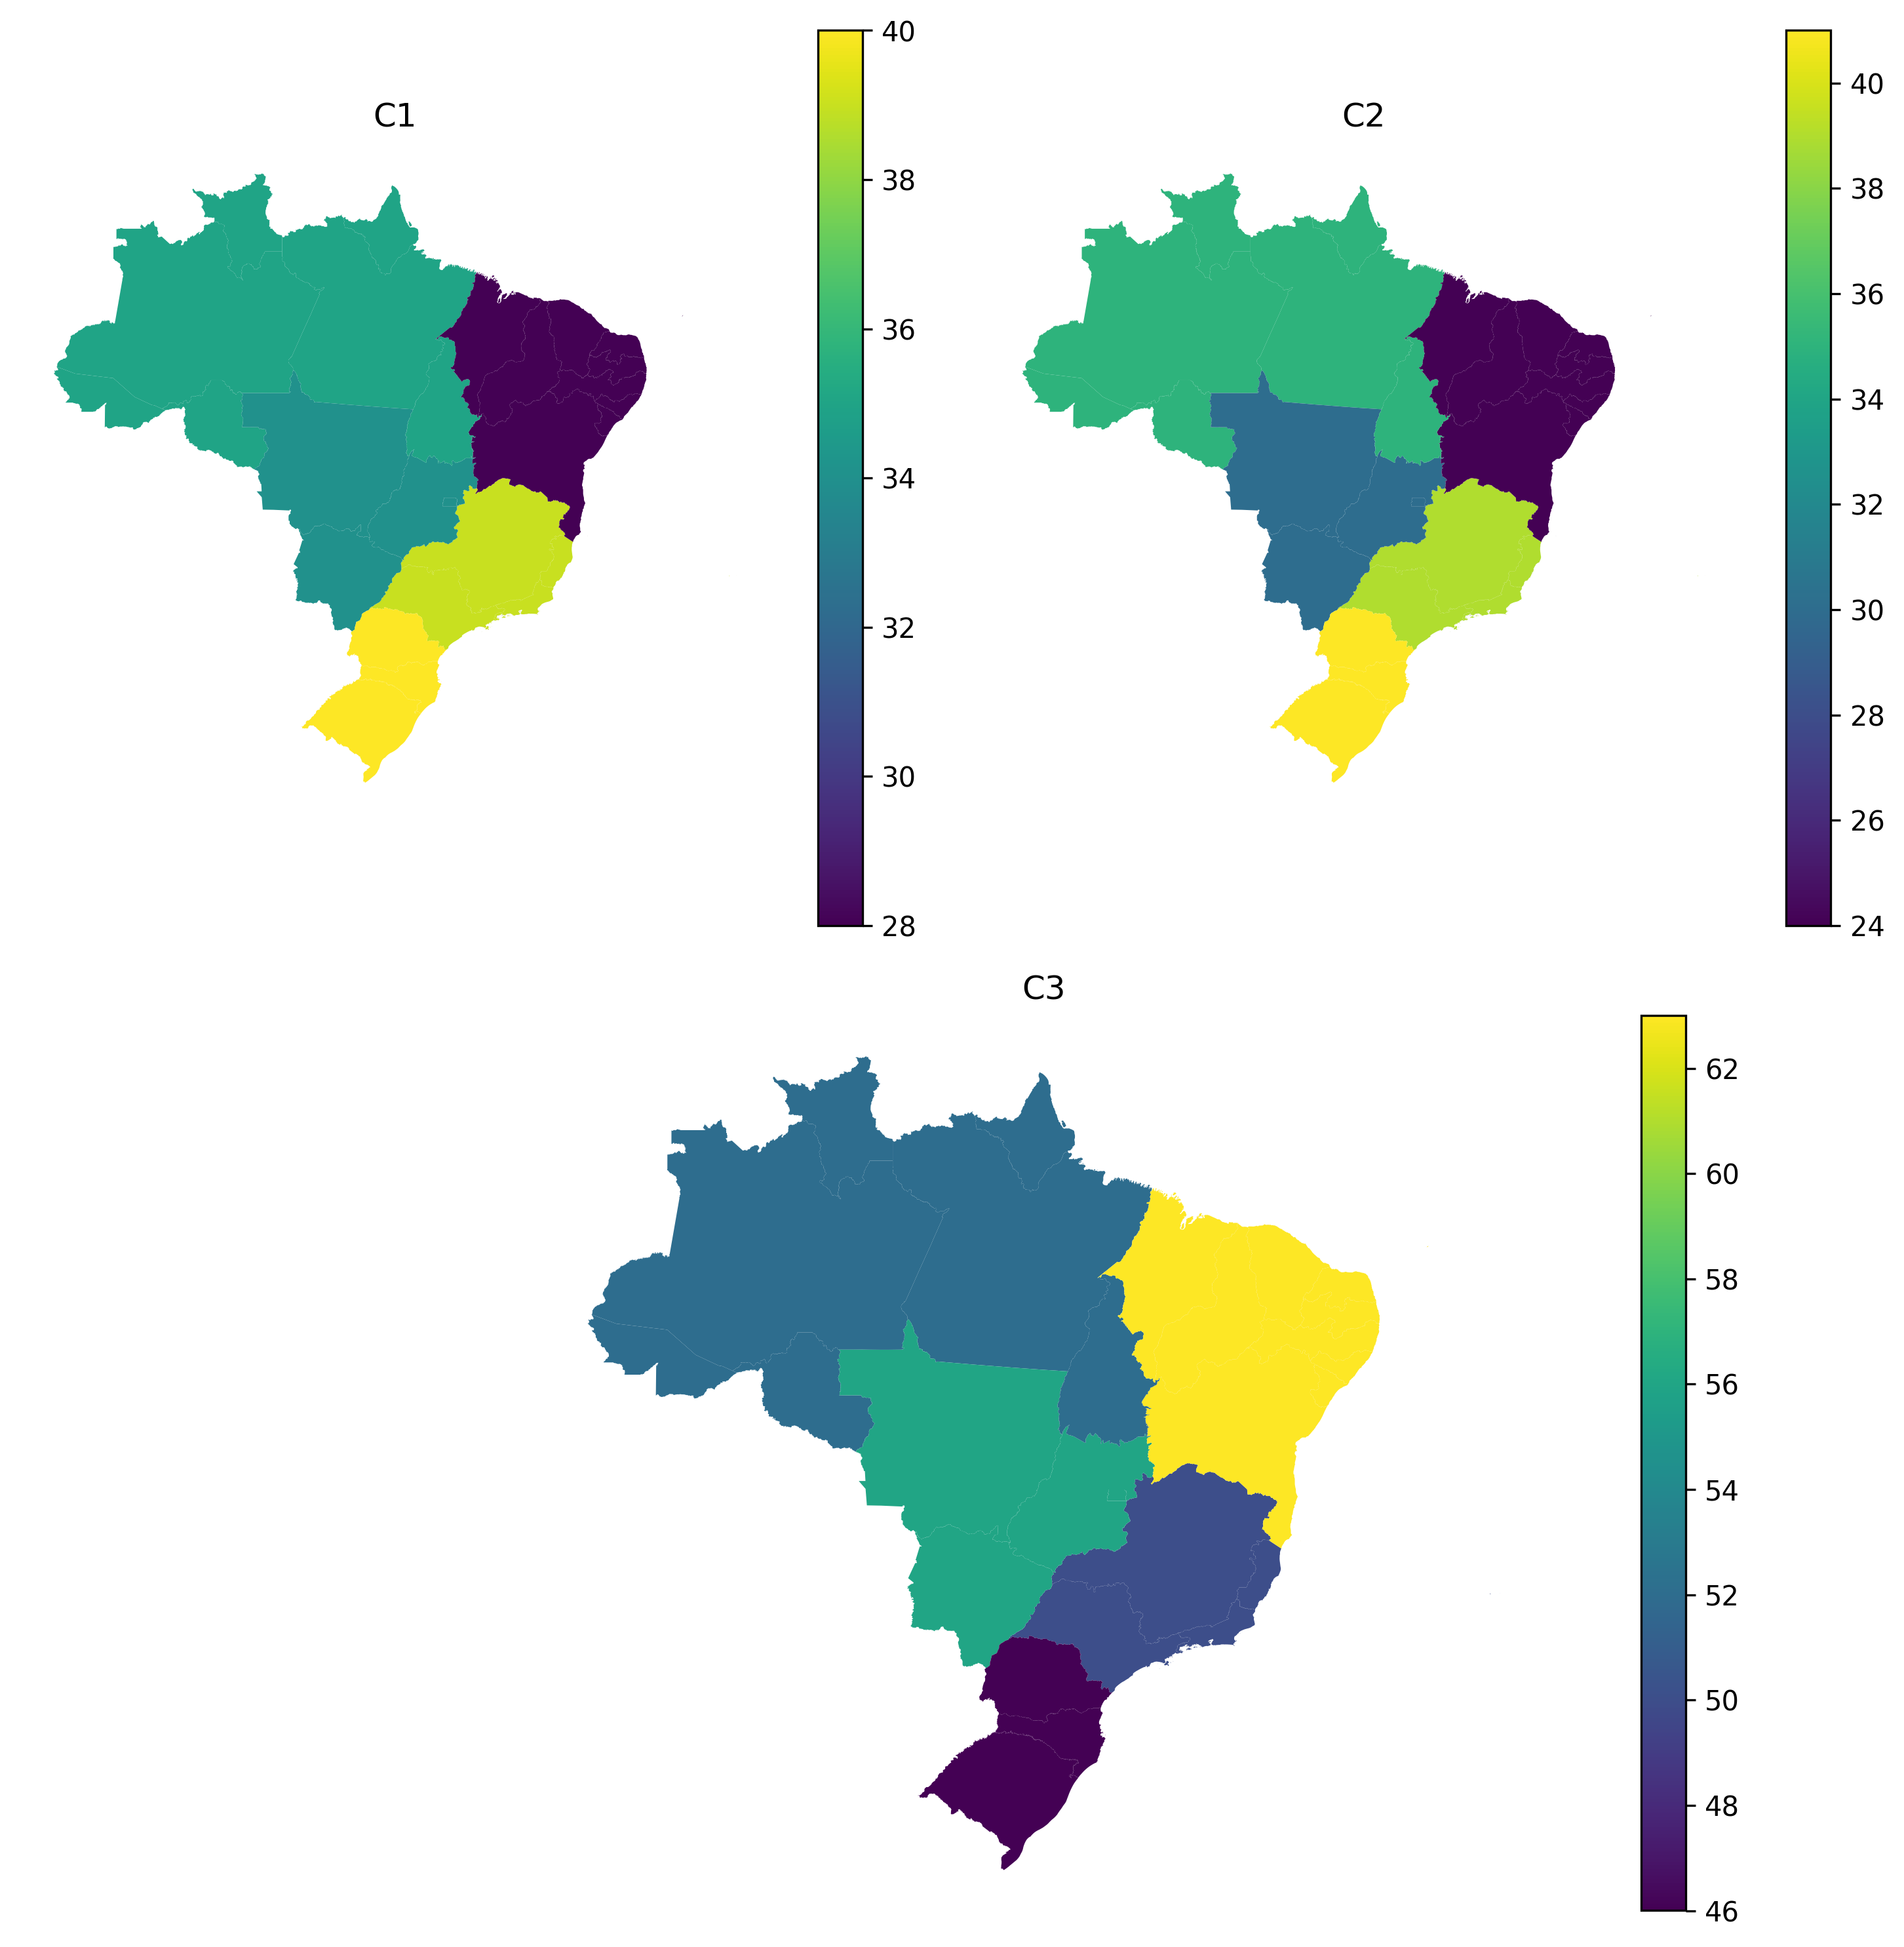
\includegraphics[width=1\linewidth]{figuras/mapa_coropletico_tic_domicilios_2024_g3.png}
	\label{fig:mapa_coropletico_tic_domicilios_2024_g3}
	\footnotesize{Fonte: elaboração própria baseade em \cite{tic_domicilios_2024_g3}.}
\end{figure}

No tocante ao critério G3-1, as regiões Sudeste e Sul foram as regiões em que mais houve procura de informações oferecidas pelo governo, seguidas do Centro-Oeste e Norte, e por fim, pelo Nordeste.

No tocante ao critério G3-2, a região Sul foi a região em que foram realizados alguns serviços públicos, como emitir documentos pela internet, preencher e enviar formulários online ou pagar taxas e impostos pela internet. A região que menos usou serviços públicos foi a Nordeste, superada pelas Centro-Oeste, Norte e Sudeste.

No tocante ao critério G3-3, o Nordeste foi a única região em que a internet não foi utilizada para interagir com as autoridades, seguido do Centro-Oeste e finalmente, o Sudeste e o Sul.

Como foi demonstrado por todas as figuras, nota-se como é notório o uso de governo eletrônico no Brasil. Tal resultado confirma a ideia de \cite{singh2007country}, que argumenta que o uso constante de governo eletrônico justifica sua existência, manutenção e evolução.

\section{Transação do governo eletrônico para o digital no Brasil}

Como expressado nos parágrafos anteriores, com as condições favoráveis, a transformação digital pode se tornar paupável, executável e planejável. Segundo \cite{mitkiewicz2024transformaccao}, a transformação digital pode ser entendida como o processo de utilização das tecnologias da informação e comunicação para gerar soluções visando resolver de forma inovadora e em larga escala os problemas do mundo.

De forma complementar, \cite{alenezi2022understanding} afirma que a transformação digital no governo ou no setor público refere-se ao engajamento diferente e inovador e o trabalho com as partes interessadas, desenvolvendo frameworks para os mecanismos de entrega de serviços eficientes e formação de novos relacionamentos.

No contexto dos parágrafos anteriores, surgem os governos digitais em substituição aos governos eletrônicos. \cite{veiga2016digital} afirma que, diferentemente do governo eletrônico, o governo digital não é apenas sobre tecnologia, é sobre uma operação multifacetada  que requer uma abordagem multidisciplinar e disciplina científica. 

\cite{bounabat2017government} complementa a ideia anterior. O auto cita que o governo digital baseia-se na divulgação aberta e sem precedentes de informações governamentais, aliada à troca em grande volume de informações altamente sensíveis e também pessoais entre agências governamentais e seus clientes. 

O governo digital traz diversos benefícios, além dos benefícios do governo eletrônico. \cite{martins2018war} argumenta que as ferramentas de governo digital promovem transparência, responsabilização e acesso melhorado à informação.

Outra vantagem é mencionada por \cite{veiga2016digital}. O autor afirma que o uso de governo digital e serviços públicos online têm um grande potencial de reduzir o fardo administrativo, bem como, promover inovação e crescimento econômico. Além de contribuir com a diminuição das atividades da economia informal, aumentando a quantidade de pessoas que pagam impostos e reduzindo a corrupção.

Para \cite{kreuz20184textordfeminine}, vive-se e assiste-se à chegada da 4ª Revolução Industrial, que imprime uma modificação substancial na forma pela qual as pessoas e os diversos sistemas se relacionam. 

Complementa \cite{kreuz20184textordfeminine} que o mundo jurídico e o poder estatal necessitam não apenas se adaptar, mas incorporar as tecnologias ao seu m\textit{modus operandi} como meio de implementar a participação social dos cidadãos no processo decisório. E assim, incorporar os preceitos reais de um constitucionalismo latino-americano.

\cite{kreuz20184textordfeminine} argumenta que o estudo de caso realizado mediante o Governo digital brasileiro fornece algumas respostas. O Brasil vem se adaptando e implementando as TICs nos seus processos de relação com a sociedade. A abertura de dados e transparência cresce a cada ano. 

\cite{kenosi2024industrial} em sua revisão da litaratura, indetificou que sua revião sistemática evidência que o potencial transformativo das tecnologias da Revolução Industrial 4.0 em melhorar os serviços de governo eletronico, focando na democrtização da administração pública vi a transparência melhorada, participação cidadã e entrega de serviços públicos.

No referido contexto, como marco legal da transição de governo eletrônico para digital  no Brasil, a \textbf{Lei do Governo Digital}, em seu artigo 1º, segundo \cite{l14129},  dispõe sobre princípios, regras e instrumentos para o aumento da eficiência da administração pública, especialmente por meio da desburocratização, da inovação, da transformação digital e da participação do cidadão.

\cite{carvalho2022nova} cita que Certamente, foi com a Lei nº 14.129, de 29 de março de 2021, que o maior passo foi dado no sentido de implantação do governo digital. A propósito, apesar de ter se autointitulado “lei do governo digital”, a citada legislação possui um campo de incidência ainda mais amplo.

Para \cite{carvalho2022nova}, no caso, o art. 1º da \textbf{Lei do Governo Digital} determina que a lei “dispõe sobre princípios, regras e instrumentos para o aumento da eficiência da administração pública”, e tal objetivo seria perseguido “especialmente por meio da desburocratização, da inovação, da  transformação digital e da participação do cidadão”. 

Para \cite{carvalho2022nova}, ademais, dentre os 26 princípios do governo digital e da eficiência pública (art. 3º), registre-se a presença tanto da “desburocratização, a modernização, o fortalecimento e a simplificação da relação do poder público com a sociedade, 
mediante serviços digitais”, como também do “incentivo à participação social no controle e na fiscalização da administração pública”.

Para \cite{carvalho2022nova}, a abertura de novos espaços de participação social na atividade administrativa do Estado trata-se de um importante passo para uma maior democratização da democracia, seja em relação ao aspecto quantitativo ou qualitativo, pois geralmente 
é a face da administração pública que apresenta o Estado ao cidadão.

\cite{carvalho2022nova} cita 4 aspectos do governo digital: 

\begin{itemize}
	\item Incremento da participação social pelo acesso dos 
cidadãos à informação e ao conhecimento
	\item A participação social digital gerando maior engajamento e 
empoderamento
	\item O governo digital aproximando a sociedade civil e o Estado
	\item Incremento da participação social viabilizada pelo monitoramento
\end{itemize}

Dos aspectos apresentados por \cite{carvalho2022nova}, será discutivo o aspecto do governo digital aproximando a sociedade civil e o Estado. Para \cite{carvalho2022nova}, um aspecto que precisa ser levado em consideração trata de uma forma de aproximação: a do Estado e da sociedade civil. Neste sentido, perceba-se que as novas tecnologias digitais não apenas permitem que a sociedade civil esteja informada, capacitada, engajada e empoderada. Elas também asseguram que o Estado possa melhor detectar qual são as aspirações dos cidadãos.

Complementarmente, para \cite{carvalho2022nova}, nesse momento de consolidação das redes sociais, vê-se a formação de uma opinião pública digital, que permite a qualquer cidadão expressar livremente suas opiniões e inclusive sugerir propostas de ação a serem adotadas pelo administrador público. O cidadão de hoje não pode apenas ser visto como um cliente da administração pública, mas sim um parceiro para a formulação e a execução de políticas estatais.

Para \cite{do2022governo}, a \text{Lei do Governo Digital}, propondo um modelo de governo digital que inaugure uma nova forma de relacionamento entre a Administração Pública e os destinatários de sua atuação, incorpora ferramentas de modificação na dinâmica tradicional regedora dessas mesmas relações.

Ainda para \cite{do2022governo}, em razão do argumento anterior, promove uma conciliação entre a racionalidade jurídica, que se encontra na regularidade do procedimento e na estabilidade das estruturas formais de organização e atuação, e a racionalidade da gestão, que tem por fonte de legitimidade a eficácia das ações desenvolvidas. 

\cite{do2022governo} elogia a mudança do paradigma legal introduzida pela \text{Lei do Governo Digital} como uma a iniciativa é de ser prestigiada, pois no alinhamento entre racionalidade jurídica e racionalidade da gestão tem-se a tradução de um direito fundamental à boa administração.

Porém, limitações para a implementação das políticas públicas de governo digital. \cite{reck2021transformaccao} cita que ainda falta muito a fazer, principalmente no que diz respeito ao processo de inclusão dos que não tem acesso aos serviços indispensáveis à busca de uma cidadania mais efetiva. 

\cite{reck2021transformaccao} complementa que o cenário do parágrafo anterior é composto por cerca de 30 milhões de pessoas, que não estão inseridos no processo democrático, em razão de não terem sido alcançados pelos serviços digitais.  Nos tempos atuais, as políticas públicas podem ser disseminadas por plataformas digitais, notadamente, pelo fato do avanço de serviços como o Governo Digital onde algumas ofertas estão cada mais exclusivas nesse meio, a citar o seguro-desemprego, meu SUS digital e previdência.

Assim, para  \cite{reck2021transformaccao}, vê-se que o exercício da cidadania para muitos, encontra obstáculos, faltando-lhes serem alcançados pelas TICs, bem como por uma educação voltada ao manejo da rede, como também, por lhes faltarem condições de acesso, especialmente à população mais vulnerável, como: negros, camponeses, ribeirinhos, povos originários, populações tradicionais, os de baixa renda; e os que mesmo tendo acesso, não tenham o necessário discernimento para fazê-lo com efetividade.

A \textbf{Lei do Governo Digital} nasceu do Projeto de Lei nº 7.843, de 2017. \cite{pl_lgd} cita como motivações para a proposição da inovação legislativa:

\begin{itemize}
    \item As críticas da qualidade ao atendimento do setor público.
    \item A precariedade e a falta de acesso a serviços públicos como fatores determinantes para o grave quadro de exclusão e desigualdade social que sempre marcou a sociedade brasileira. 
    \item  A simplificação das relações entre pessoas,
    sejam elas físicas ou jurídicas, com o poder público, tema essencial para o acesso a direitos básicos e, principalmente, para o desenvolvimento econômico.
    \item O excesso de exigências burocráticas, a baixa informatização, o ainda frágil acesso à informação, a falta de abertura das bases de dados públicos, a ausência de mecanismos de participação e inovação, além da corrupção, são alguns dos problemas que explicam a precariedade e ineficiência dos serviços públicos prestados
    nas três esferas da federação.
\end{itemize}

Nesse sentido, a \textbf{Lei do Governo Digital}, visando melhorar a administração pública, seu artigo 5º, conforme \cite{l14129}, serão utilizadas soluções digitais para a gestão de suas políticas finalísticas e administrativas e para o trâmite de processos administrativos eletrônicos.

Além disso, \textbf{Lei do Governo Digital}, segundo \cite{l14129}, determina sua aplicação às Administrações Direta e Indireta da União Federal e dos demais entes federados, desde que adotem os comandos da lei por meio de atos normativos próprios, vedada a aplicação da lei às empresas públicas e sociedades de economia mista, suas subsidiárias e controladas que não prestem serviço público.

Haja vista \cite{reck2021transformaccao}, o governo digital não se restringe à automação de processos e à disponibilização de serviços públicos on-line, busca avançar para um modelo de administração pública capaz de integrar as TICs a seus processos internos e aos cidadãos, buscando cumprir os papéis essenciais do Estado de forma mais eficiente, bem como restar serviços públicos mais qualificados. 

De forma complementar ao argumento anterior, \cite{lima2023governo}, com as inovações legislativas trazidas pela \textbf{Lei do Governo Digital}, especialmente com o enfoque em um modelo do Governo digital por plataforma, notadamente na esfera federal, a mudança está em sintonia com as mudanças tecnológicas, principalmente impulsionadas pela pandemia da Covid-19, guarda estrita sintonia com a ordem jurídica constitucional vigente e evidencia essa ordem de preocupação normativa da parte do Poder Público.

A maneira como o poder público se relaciona com a sociedade civil, sob a ótica do governo digital, segundo  \cite{lima2023governo}, é via as plataformas de governo digital, pois constituem realizações que buscam a aproximação entre Administração e cidadãos e cidadãs na esfera digital e, adicionalmente, são os meios pelos quais a atuação pública alcança suas finalidades.

Para \cite{de2020governo}, ao longo dos anos, a administração pública no Brasil se estruturou e foi moldada a partir de um amálgama entre uma concepção jurídica formalista, práticas burocráticas e uma generalizada cultura da desconfiança. 

\cite{de2020governo} complementa a ideia anterior citando as diversas faces 
conhecidas do modelo democrático:  

\begin{itemize}
    \item Interpretações e decisões baseadas em conceitos abstratos, ignorando as suas consequências práticas, defesa de ritos e formas como um fim em si mesmo, exigências de regularização desnecessárias.
    \item Um ambiente institucional que incentiva e premia o conservadorismo e a apatia de servidores e gestores públicos.
\end{itemize}

\cite{de2020governo} argumenta que as iniciativas de governo digital - sucessoras do governo eletrônico - pretendem, justamente, transformar a realidade do modelo burocrático inefetivo, eficaz  e ineficiente, mediante a instituição de serviços públicos digitais, que sejam mais simples, céleres e eficientes.

A implementação das iniciativas de governo digital trata-se, segundo \cite{de2020governo}, da construção de um novo paradigma  de administração pública, fundado sobre os princípios da transparência, da inovação e da confiança  segundo os quais o uso das tecnologias digitais pode e deve viabilizar: 

\begin{itemize}
    \item A ampliação do acesso às informações públicas e a simplificação de 
    mecanismos de prestação de contas e de interação entre a administração 
    pública e a sociedade, incluindo a instituição de novos mecanismos de 
    avaliação dos serviços.
    \item A efetiva e constante inovação, mediante a adoção de modelos 
    administrativos e jurídicos flexíveis, a admissibilidade controlada do risco, a relativa tolerância ao erro, o questionamento de práticas vigentes e a criação de incentivos para a experimentação e para a implementação de soluções criativas por parte de gestores públicos.
    \item Com base na arquitetura disponibilizada pelas tecnologias digitais, a constituição de novos modos de produção da confiança, por meio dos quais seja possível a redução de exigências burocráticas, bem como a garantia de maior simplicidade, celeridade, previsibilidade e segurança nas relações entre cidadãos e órgãos e entidades públicos.
\end{itemize}

Relativo ao primeiro tópico, o Brasil sanou o problema citado com a aprovação da Lei nº 12.527, de 2011 - Lei de Acesso à Informação e com a implementação dos portais da transparência do órgãos e Poderes dos Entes Federados.

O segundo tópico foi sanado pelo \textbf{Lei do Governo Digital} pela criação dos laboratórios de inovação. Para \cite{l14129}, laboratório de inovação é um espaço aberto à participação e à colaboração da sociedade para o desenvolvimento de ideias, de ferramentas e de métodos inovadores para a gestão pública, a prestação de serviços públicos e a participação do cidadão no exercício do controle sobre a administração pública.

O último e terceiro tópico foi sanado com a determinação legal de que apenas o CPF, para pessoas físicas, e o CNPJ, para pessoas jurídicas, como a única forma de identificação aceita pela administração pública, haja vista a \textbf{Lei do Governo Digital} (art. 28, \textbf{caput}), conforme exposto por \cite{l14129}: "Art. 28.  Fica estabelecido o número de inscrição no Cadastro de Pessoas Físicas (CPF) ou no Cadastro Nacional da Pessoa Jurídica (CNPJ) como número suficiente para identificação do cidadão ou da pessoa jurídica, conforme o caso, nos bancos de dados de serviços públicos, garantida a gratuidade da inscrição e das alterações nesses cadastros."

Independentemente dos benefícios apresentados pelos argumentos anteriores, considerando \cite{de2020governo} a ideia de que há diversos obstáculos que podem dificultar ou desvirtuar o sentido e os resultados das políticas de governo digital, dentre elas: o risco de digitalização de fachada e se foi realizada sem as devidas salvaguardas técnicas e jurídicas.

No tocante ao risco de digitalização de fachada, segundo \cite{de2020governo}, pode ocorrer a manutenção da lógica burocrática tradicional sob uma roupagem eletrônica, equívoco muitas vezes encontrado na administração pública brasileira. O segundo problema, a incorporação de tecnologias digitais pode gerar externalidades negativas, produzindo novos riscos e incertezas ou, ainda, abusos e violação de direitos.

Outros fatores são citados como barreiras para a implementação das políticas de governo digital, são para \cite{do2022governo}: 

\begin{itemize}
    \item No campo da resistência cultural, o investimento, obrigatoria
    mente, deve ser no treinamento e na formação das lideranças públicas 
    a conduzirem o processo.
    \item Na relação com o controle, as iniciativas associadas 
    ao governo digital devem se pautar, principalmente, pelo sempre pres
    tigiado vetor da transparência
\end{itemize}

No tocante ao primeiro tópico, \cite{do2022governo} afirma que o investimento, obrigatoriamente, deve ser no treinamento e na formação das lideranças públicas 
a conduzirem o processo. Educação digital deve ser a palavra de ordem dentro da Administração, para os seus próprios agentes, e em favor dos destinatários do governo digital. 

Como resultado da educação para mitigar a resistência à digitalização do poder público, segundo \cite{do2022governo}, ampliada a educação digital, o valor inerente ao governo de mesmo cariz resta autoevidente, e com isso a tendência é de mitigação da resistência a partir da perspectiva de constrição fiscal.

No tocante ao segundo e último tópico, \cite{do2022governo} argumenta que na relação com o controle, principalmente, pelo sempre prestigiado vetor da transparência. O problema não está em navegar em mares nunca dantes navegados, mas sim, em não ter clareza quanto às ondas que se possam ter pela frente.

\bibliography{ref}
\bibliographystyle{acm}

\end{document}
